\documentclass[12pt]{ucdavisthesis}

% PLEASE READ THE MANUAL - ucdavisthesis.pdf (in the package installation directory)

%%%%%%%%%%%%%%%%%%%%%%%%%%%%%%%%%%%%%%%%%%%%%%%%%%%%%%%%%%%%%%%%%%%%%%%%
%                                                                      %
%               LATEX COMMANDS FOR DOCUMENT SETUP                      %
%                                                                      %
%%%%%%%%%%%%%%%%%%%%%%%%%%%%%%%%%%%%%%%%%%%%%%%%%%%%%%%%%%%%%%%%%%%%%%%%

%\usepackage{bookmark}
\usepackage[us,nodayofweek,12hr]{datetime}
\usepackage{graphicx}
\usepackage[square,comma,numbers,sort&compress]{natbib}
\usepackage{gensymb}
%\usepackage{hypernat}
% Other useful packages to try
\usepackage{amsmath}
%\usepackage{amssymb}
\usepackage{textcomp}
%
% Different fonts to try (uncomment only fontenc and one font at a time)
% (you may need to install these first)
\usepackage[T1]{fontenc} %enable fontenc package if using one of the fonts below
%\usepackage[adobe-utopia]{mathdesign}
\usepackage{tgschola}
%\usepackage{tgbonum}
%\usepackage{tgpagella}
%\usepackage{tgtermes}
%\usepackage{fourier}
%\usepackage{fouriernc}
%\usepackage{kmath,kerkis}
%\usepackage{kpfonts}
%\usepackage[urw-garamond]{mathdesign}
%\usepackage[bitstream-charter]{mathdesign}
%\usepackage[sc]{mathpazo}
%\usepackage{mathptmx}
%\usepackage[varg]{txfonts}

%%Packages that I added
\usepackage[section]{placeins} %keeps floats from bein gplaced outside the sections they are placed in.
\usepackage{fancyhdr}
\usepackage{siunitx} %used by glossary
\usepackage[acronyms,nogroupskip,nonumberlist]{glossaries}
\setlength{\glsdescwidth}{0.8\linewidth}
\glsaddkey{unit}{\glsentrytext{\glslabel}}{\glsentryunit}{\GLsentryunit}{\glsunit}{\Glsunit}{\GLSunit}
\makeglossaries
\glsaddall %Include all glossary entries in glossary. This needs to be here for correct page layout during document compiling, but needs to be after \begin{document} to create List of abbreviations input file.
\overfullrule=0pt

%Symbols%%%%%%%%%%%%%%%%%%%%%%%%%%%%%%%%%%%%%%%%%%%%%%%%%%%%%%%%
\newglossaryentry{a}{name={$U$},		description={incoming wind speed at the turbine rotor},		unit={$m{\cdot}s^{-1}$}}
\newglossaryentry{b}{name={$R$},		description={rotor radius},		unit={$m$}}
\newglossaryentry{c}{name={$C_p$},		description={coefficient of power},		unit={$-$}}
\newglossaryentry{d}{name={$D$},		description={downwind distance between turbines},		unit={$m$}}
\newglossaryentry{e}{name={$U_{conv}$},		description={convection speed},		unit={$m{\cdot}s^{-1}$}}
\newglossaryentry{f}{name={$U_{mean}$},		description={local mean wind speed},		unit={$m{\cdot}s^{-1}$}}
\newglossaryentry{g}{name={$U_{turb}$},	description={wind speed fluctuations due to turbulence},		unit={$m{\cdot}s^{-1}$}}
\newglossaryentry{h}{name={$U_{ff}$},	description={feed forward wind speed estimate supplied by upwind turbine},		unit={$m{\cdot}s^{-1}$}}
\newglossaryentry{i}{name={$\theta$},	description={collective blade pitch angle of the turbine},		unit={$deg$}}
\newglossaryentry{j}{name={$\Omega _{Rotor}$},	description={rotational speed of the rotor},		unit={$rad{\cdot}s^{-1}$}}
\newglossaryentry{k}{name={$T_{Gen}$},	description={torque supplied by the generator},		unit={$N{\cdot}m$}}
\newglossaryentry{l}{name={$I_{Drivetrain}$},	description={low speed shaft equivalent inertia},		unit={$kg{\cdot}m^{2}$}}
\newglossaryentry{m}{name={$T_{Aero}$},	description={aerodynamic torque on the rotor due to the wind},		unit={$N{\cdot}m$}}
\newglossaryentry{n}{name={$N_{Gear}$},	description={gear box ratio},		unit={$-$}}
\newglossaryentry{o}{name={$\rho$},	description={air density},		unit={$kg{\cdot}m^{-3}$}}
\newglossaryentry{p}{name={$R$},	description={rotor radius},		unit={$m$}}
\newglossaryentry{q}{name={$\lambda$},	description={tip speed ratio},		unit={$-$}}
\newglossaryentry{r}{name={$t_D$},	description={time required for a gust to pass from the upwind to downwind turbine},		unit={$s$}}
\newglossaryentry{s}{name={$\theta_{ff}$},	description={pitch command issued by the feed forward controller},		unit={$deg$}}
\newglossaryentry{t}{name={$\theta_{c}$},	description={pitch command issued by the closed loop controller},		unit={$deg$}}
\newglossaryentry{u}{name={$T_{ff}$},	description={torque command issued by the feed forward controller},		unit={$N{\cdot}m$}}
\newglossaryentry{v}{name={$\xi$},	description={damping ratio of the pitch actuator},		unit={$-$}}
\newglossaryentry{w}{name={$\omega_o$},	description={undamped natural frequency of the pitch actuator},		unit={$Hz$}}
\newglossaryentry{x}{name={$\theta_{ss}$},	description={steady state pitch function},		unit={$deg$}}
\newglossaryentry{y}{name={$U_{ffd}$},	description={dynamic feed forward velocity},		unit={$m{\cdot}s^{-1}$}}
\newglossaryentry{z}{name={$\Omega _{Gen}$},	description={rotational speed of the generator},		unit={$rad{\cdot}s^{-1}$}}
\newglossaryentry{aa}{name={$\Omega _{GenFilt}$},	description={low pass filtered rotational speed of the generator},		unit={$rad{\cdot}s^{-1}$}}
\newglossaryentry{ab}{name={$D_{fatigue}$},	description={total damage due to cyclic loading},		unit={$-$}}
\newglossaryentry{ac}{name={$N_{fatigue, i}$},	description={number of cycles to failure for the $i^th$ loading cycle},		unit={$-$}}
\newglossaryentry{ad}{name={$L_{ultimate}$},	description={ultimate design load},		unit={$-$}}
\newglossaryentry{ae}{name={$L_{mean}$},	description={mean load over a components load history},		unit={$-$}}
\newglossaryentry{af}{name={$L_{range,i}$},	description={range of a cyclic load},		unit={$-$}}
\newglossaryentry{ag}{name={$N_{equivalent}$},	description={number of cycles to failure for the damage equivalent load},		unit={$-$}}
\newglossaryentry{ah}{name={$m$},	description={W\"{o}hler exponent},		unit={$-$}}
\newglossaryentry{ai}{name={$\Omega _{GenR}$},	description={rated rotational speed of the generator},		unit={$rad{\cdot}s^{-1}$}}
\newglossaryentry{aj}{name={$\Omega _{GenR\_Derated}$},	description={rated rotational speed of the generator when derated},		unit={$rad{\cdot}s^{-1}$}}
\newglossaryentry{ak}{name={$\eta\_{DR}$},	description={derate factor},		unit={$-$}}
\newglossaryentry{al}{name={$k_{gen}$},	description={region 2 generator torque constant},		unit={$N{\cdot}m{\cdot}s^2{\cdot}rad^{-2}$}}
\newglossaryentry{am}{name={$k_{gen\_Derated}$},	description={region 2 generator torque constant when derated},		unit={$N{\cdot}m{\cdot}s^2{\cdot}rad^{-2}$}}
\newglossaryentry{an}{name={$t_{Event}$},	description={time when upwind turbine detects an extreme wind event},		unit={$s$}}
\newglossaryentry{ap}{name={$t_{DR\_start}$},	description={time when downwind turbine begins derating},		unit={$s$}}
\newglossaryentry{aq}{name={$t_{DR\_end}$},	description={time when downwind turbine begins return to full rating},		unit={$s$}}
\newglossaryentry{ar}{name={$t_{conv}$},	description={estimate time for gust to travel between turbines},		unit={$s$}}
\newglossaryentry{as}{name={$t_{s}$},	description={time required for turbine to transition into/out of derated opertion},		unit={$s$}}





%Abbreviations%%%%%%%%%%%%%%%%%%%%%%%%%%%%%%%%%%%%%%%%%%%%%%%%%%%
\newacronym{BRM}{BRM}{\textbf{B}lade \textbf{R}oot bending \textbf{M}oment}
\newacronym{CFD}{CFD}{\textbf{C}omputational \textbf{F}luid \textbf{D}ynamics}
\newacronym{CGT}{CGT}{\textbf{C}himera \textbf{G}rid \textbf{T}ools}
\newacronym{COE}{COE}{\textbf{C}ost \textbf{O}f \textbf{E}nergy}
\newacronym{DEL}{DEL}{\textbf{D}amage  \textbf{E}quivalent \textbf{L}oad}
\newacronym{ECG}{ECG}{\textbf{E}xtreme  \textbf{C}oherent \textbf{G}ust}
\newacronym{EOG}{EOG}{\textbf{E}xtreme  \textbf{O}perating \textbf{G}ust}
\newacronym{FAST}{FAST}{\textbf{F}atigue,  \textbf{A}erodynamics, \textbf{S}tructures, and  \textbf{T}urbulence}
\newacronym{IEC}{IEC}{\textbf{I}nternational  \textbf{E}lectrotechnical \textbf{C}ommission}
\newacronym{LES}{LES}{\textbf{L}arge  \textbf{E}ddy \textbf{S}imulation}
\newacronym{NREL}{NREL}{\textbf{N}ational \textbf{R}enewable \textbf{E}nergy  \textbf{L}aboratory}
\newacronym{NWTC}{NWTC}{\textbf{N}ational \textbf{W}ind \textbf{T}echnology  \textbf{C}enter}
\newacronym{PI}{PI}{\textbf{P}roportional and  \textbf{I}ntegral (Control)}
\newacronym{RANS}{RANS}{\textbf{R}eynolds  \textbf{A}veraged \textbf{N}avier \textbf{S}tokes}
\newacronym{SOWFA}{SOWFA}{\textbf{S}imulator  f\textbf{O}r \textbf{W}ind  \textbf{F}arm  \textbf{A}pplications}
\newacronym{SST}{SST}{\textbf{S}hear  \textbf{S}tress \textbf{T}ransport}
\newacronym{GPLLJ }{GPLLJ }{\textbf{G}reat  \textbf{P}lains \textbf{L}ow \textbf{L}evel \textbf{J}et }
 
%GLossary style to use units

\newglossarystyle{symbunitlong}{%
\setglossarystyle{long3col}% base this style on the list style
\renewenvironment{theglossary}{% Change the table type --> 3 columns
  \begin{longtable}{lp{0.8\glsdescwidth}>{\centering\arraybackslash}p{2cm}}}%
  {\end{longtable}}%
%
%\renewcommand*{\glossaryheader}{%  Change the table header
%  \bfseries Sign & \bfseries Description & \bfseries Unit \\
%  \hline
%  \endhead}
\renewcommand*{\glossentry}[2]{%  Change the displayed items
\glstarget{##1}{\glossentryname{##1}} %
& \glossentrydesc{##1}% Description
& \glsunit{##1}  \tabularnewline
}
}



\hyphenation{dis-ser-ta-tion blue-print man-u-script pre-par-ing} %add hyphenation rules for words TeX doesn't know


\renewcommand{\rightmark}{\scriptsize A University of California Davis\ldots \hfill Rev.~\#2.0 \quad Compiled: \currenttime, \today}
% a fancier running header that can be used with draftcls options

%%%%%%%%%%%%%%%%%%%%%%%%%%%%%%%%%%%%%%%%%%%%%%%%%%%%%%%%%%%%%%%%%%%%%%%%
%                                                                      %
%        DOCUMENT SETUP AND INFORMATION FOR PRELIMINARY PAGES          %
%                                                                      %
%%%%%%%%%%%%%%%%%%%%%%%%%%%%%%%%%%%%%%%%%%%%%%%%%%%%%%%%%%%%%%%%%%%%%%%%

\title          {Feed Forward Wind Turbine Control \\
				Using Upwind Turbines as Sensors}
%Exact title of your thesis. Indicate italics where necessary by underlining or using italics. Please capitalize the first letter of each word that would normally be capitalized in a title.

\author         {Eric William Anderson}
%Your full name as it appears on University records. Do not use initials.

\authordegrees  {B.S. (University of California, Berkeley) 2000 \\
                 M.S. (Georgia Institute of Technology) 2004}
%Indicate your previous degrees conferred.

\officialmajor  {Mechanical and Aerospace Engineering}
%This is your official major as it appears on your University records.

\graduateprogram{Mechanical and Aerospace Engineering}
%This is your official graduate program name. Used for UMI abstract.

\degreeyear     {2017}
% Indicate the year in which your degree will be officially conferred.

\degreemonth    {September}
% Indicate the month in which your degree will be officially conferred. Used for UMI abstract.

\committee{Professor C.P. van Dam}{Professor Stephen K. Robinson}{Dr. David Maniaci}{}{}
% These are your committee members. The command accepts up to five committee members so be sure to have five sets of braces, even if there are empties.

%%%%%%%%%%%%%%%%%%%%%%%%%%%%%%%%%%%%%%%%%%%%%%%%%%%%%%%%%%%%%%%%%%%%%%%%

%\copyrightyear{2020}
%\nocopyright

%%%%%%%%%%%%%%%%%%%%%%%%%%%%%%%%%%%%%%%%%%%%%%%%%%%%%%%%%%%%%%%%%%%%%%%%

%\dedication{\textsl{To someone very important \ldots \\
%            a nice dedication.}}

%%%%%%%%%%%%%%%%%%%%%%%%%%%%%%%%%%%%%%%%%%%%%%%%%%%%%%%%%%%%%%%%%%%%%%%%

\abstract{This dissertation seeks to improve the performance of a downwind turbine using information obtained from an upwind turbine. Methods for using an upwind turbine as a sensor are examined and evaluated. Next, a feed forward optimum pitch control scheme is introduced and investigated using a series of FAST simulations. In this control scheme an upwind is used as a wind speed sensor. Wind speed measurements are passed from the upwind turbine to a downwind turbine. The downwind turbine uses the knowledge of incoming wind speed to proactively adjust turbine blade pitch. Initial simulations are promising, but ultimately the feed forward control system is found to be very sensitive to timing errors. This make the control scheme impractical in real world applications. A feed forward derating control scheme is then developed. In this control scheme the rotor speed of the upwind turbine is monitored for evidence of an extreme gust event. If an extreme gust is detected the downwind turbine is derated to mitigate the negative effects of the gust. A series of FAST simulations show that this control scheme can reduce structural loads and rotor overspeeds in the downwind turbine. Unlike feed forward optimal pitch control, this system is insensitive to timing errors. A more sophisticated wind farm simulation tool, SOWFA, is then used to simulate and evaluate feed forward derating control. First, a verification and validation study of SOWFA is carried out. Good agreement is found between SOWFA, OVERFLOW2 and FAST results. SOWFA is then used to simulate two test cases where turbines are subjected to extreme coherent gusts. In both test cases feed forward derating control significantly improves performance, reducing damage equivalent loads and increasing energy capture.}

%%%%%%%%%%%%%%%%%%%%%%%%%%%%%%%%%%%%%%%%%%%%%%%%%%%%%%%%%%%%%%%%%%%%%%%%

%\acknowledgments{Acknowledgements to those who helped you get to this point. They should be listed by chapter when appropriate.}

%%%%%%%%%%%%%%%%%%%%%%%%%%%%%%%%%%%%%%%%%%%%%%%%%%%%%%%%%%%%%%%%%%%%%%%%

% Each chapter can be in its own file for easier editing and brought in with the \include command.
% Then use the \includeonly command to speed compilation when working on a particular chapter.
% \includeonly{Appendices/AppendixB}

\AtBeginEnvironment{table}{\singlespacing}

\begin{document}

%\glsaddall %Include all glossary entries in glossary. This needs to be here to create List of ymbols input file, but need to not be here for correct page layout during document compiling.

\renewcommand{\bibfont}{\singlespacing}
% need this command to keep single spacing in the bibliography when using natbib

\bibliographystyle{unsrtnat}
%many other bibliography styles are available (IEEEtran, mla, unsrtnat, etc.). Use one appropriate for your field.

\makeintropages %Processes/produces the preliminary pages



%----------------------------------------------------------------------------------------
%	THESIS CONTENT - CHAPTERS
%----------------------------------------------------------------------------------------

% Chapter Template

\chapter{Introduction and Background} % Main chapter title

\label{Chapter1} % Change X to a consecutive number; for referencing this chapter elsewhere, use \ref{ChapterX}

%----------------------------------------------------------------------------------------
%	SECTION 1
%----------------------------------------------------------------------------------------

\section{Wind Power}

Wind power is the fastest growing energy source in the world.  From 2000 to 2015, global wind power capacity grew from 17,400MW to 432,883MW, with an average increase of 24\% per year (Figure \ref{fig1-1} ). In 2015, the increase in wind generation was equal to almost half of global electricity growth\cite{sawyer2015}. In the United States, installed wind capacity grew from approximately 2,500 MW in the year 2000 to 82,143 MW in 2016 \cite{williams2016}. Though wind power only represents a small fraction of total global power generation, it is an important source of clean renewable energy and its importance will increase in the future.

\begin{figure}[htbp]
	\centering
		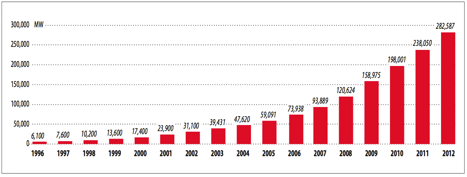
\includegraphics[width=\linewidth]{Figures/ch1Figures/fig1-1.png}
	\caption{Global wind power capacity. \cite{sawyer2015}}
	\label{fig1-1}
\end{figure}

Much of wind power$'$s success is due to two factors: the widespread availability of wind resources and the relatively low Cost of Energy (COE) when compared to other renewable energy sources.  For example, utility scale wind energy typically costs 5-12 cents per KW-hr while utility scale solar-PV typically costs 15-30 cents per KW-hr \cite{ren212011}. Though some renewable energy sources such as geothermal plants or large hydro plants can produce energy at lower COE than wind farms, the natural resources needed for those plants are much more limited.  

The cost of wind power has been steadily decreasing.  The decreases in wind power COE have gone hand in hand with increases in both the size and complexity of wind turbines.  As the turbines have grown in size and complexity, more sophisticated methods for controlling those turbines have been required.  


%----------------------------------------------------------------------------------------
%	SECTION 2
%----------------------------------------------------------------------------------------

\section{Wind Turbine Control} \label{section1-2} 

A control system typically consists of sensors, actuators, and a controller. A modern wind turbine might include sensors such as: an anemometer, a wind vane, at least one rotor speed sensor, an electric power sensor, accelerometers, load sensors, pitch position sensors, various limit switches, vibration sensors, temperature and oil level indicators, hydraulic pressure sensors, operator switches, and push buttons.  Actuators might include:  hydraulic or electric pitch actuators, an electric generator that can actively control generator torque, generator contacts, switches for activating shaft brakes, and yaw motors.  The controller collects information from sensors, processes that data, the issues commands to actuators. For a wind turbine, the controller typically consists of a computer based controller used for normal operation, and a highly reliable hard wired safety system that overrides the computer based controller and brings the turbine to a safe state if a serious problem occurs.\cite{burton2011}

The control system performs a variety of functions, but this research is primarily concerned with the closed loop control system that optimizes turbine performance during power production. The majority of utility scale turbines built today use variable speed and collective pitch to feather control.  In this control scheme both the rotational speed of the turbine and the collective pitch of the turbine$'$s three blades are controlled. At low and medium wind speeds the pitch is held constant while the turbine speed is varied.  At high wind speeds both the turbine speed and the blade pitch can be varied.

At low and medium wind speeds, the rotational speed of the rotor is manipulated to maximize aerodynamic efficiency and maximize energy capture.  The variations in rotational speed are achieved by torque control, which is implemented by using a pre-determined generator torque vs. generator speed curve like the one shown in Figure \ref{fig1-2}.  The torque controller receives measurements from a generator speed sensor, looks up the appropriate generator torque on the speed-torque curve and commands the generator to produce that torque. The blue line in Figure \ref{fig1-2} shows the torque vs. speed curve for the torque controller on the NREL 5-MW reference turbine.  The black line shows the torque-speed curve corresponding to maximum aerodynamic efficiency of the turbine. Figure \ref{fig1-3} shows the relationship between generator speed and generated power. In region 1 the generator produces no torque and no power, in region 2 the generator tracks optimum aerodynamic efficiency, and in region 3 the generator tracks constant power output.  Regions 1.5 and 2.5 simply serve as smooth transitions between the other regions. 



\begin{figure}[htbp]
	\centering
		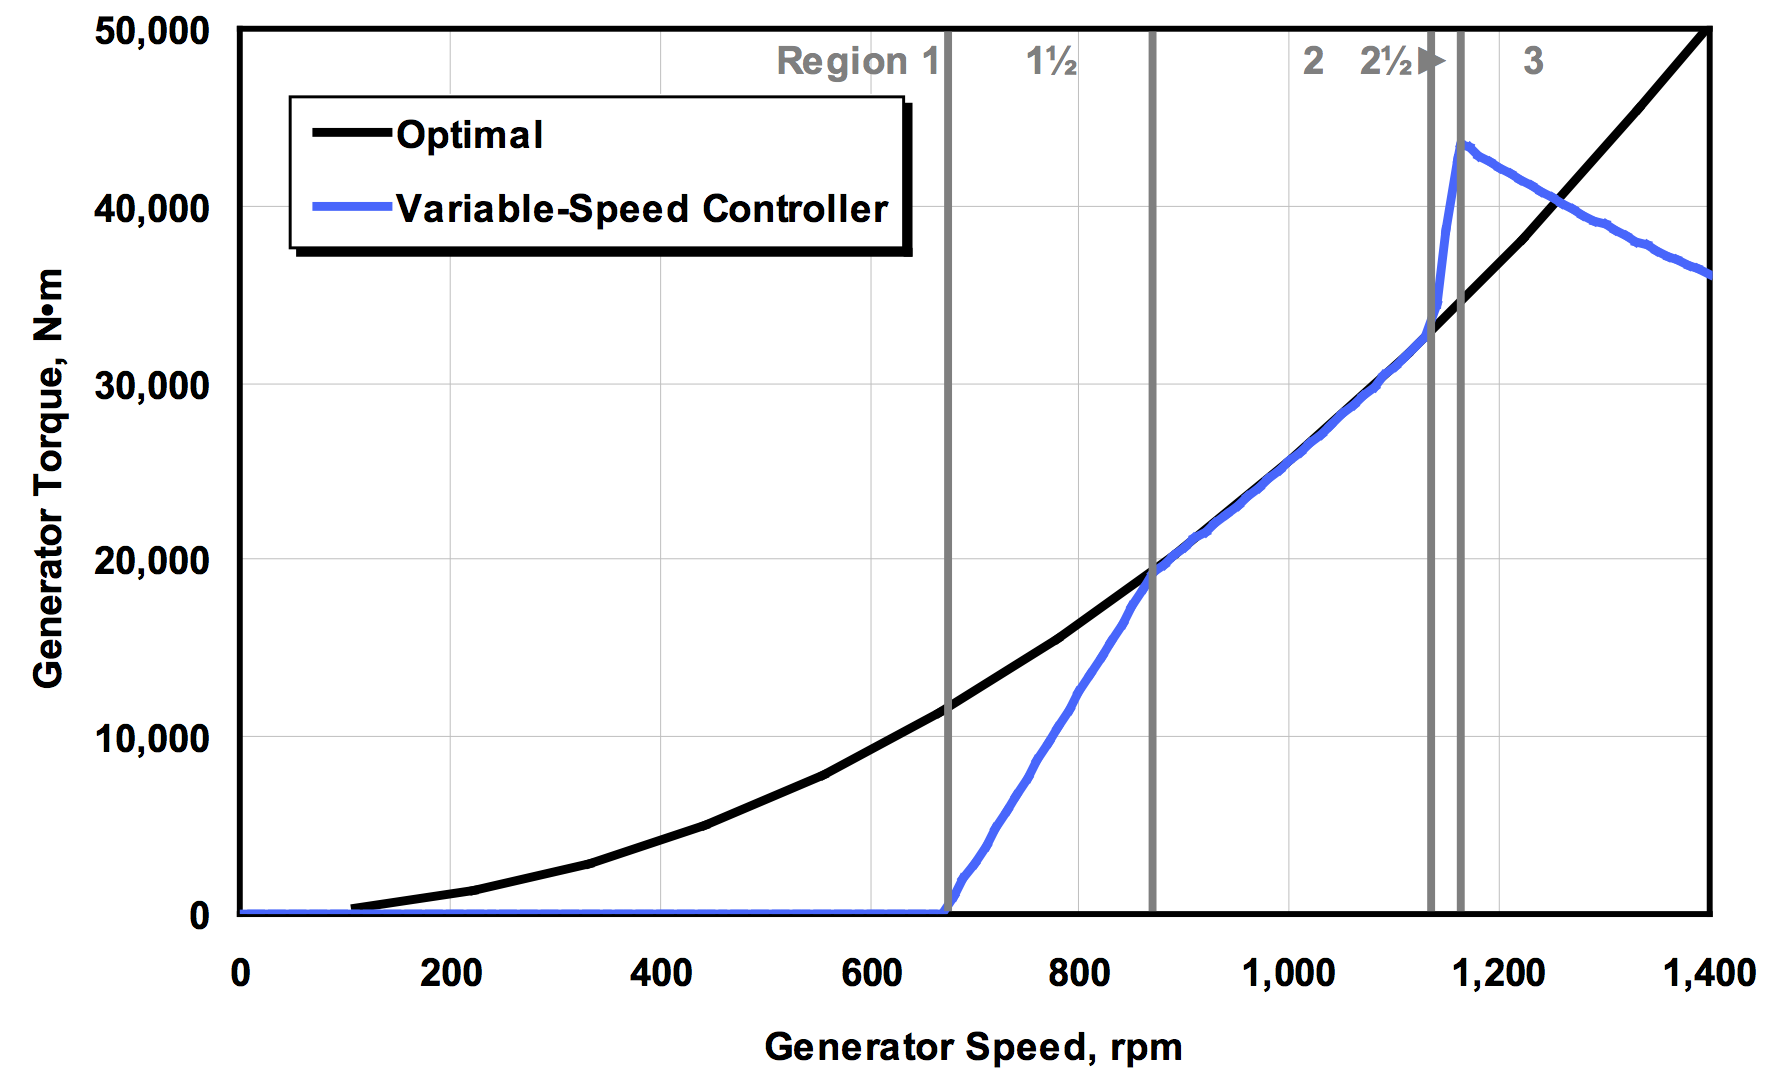
\includegraphics[width=.75\linewidth]{Figures/ch1Figures/fig1-2.png}
	\caption{Torque-speed curve for NREL 5-MW turbine.\cite{jonkman2009}}
	\label{fig1-2}
\end{figure}

\begin{figure}[htbp]
	\centering
		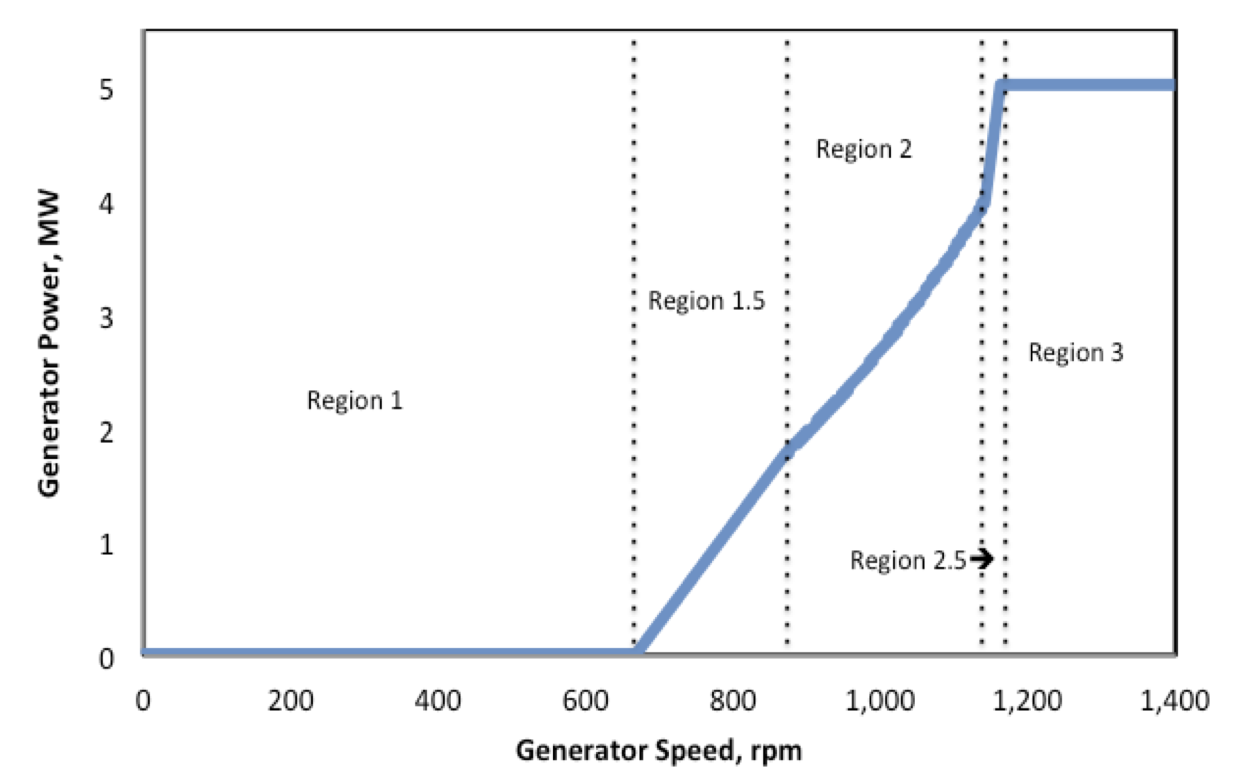
\includegraphics[width=.75\linewidth]{Figures/ch1Figures/fig1-3.png}
	\caption{Power-speed curve for NREL 5-MW turbine.}
	\label{fig1-3}
\end{figure}

At high wind speeds the collective blade pitch is manipulated to keep turbine speed and power generation constant. As wind speed increases, the turbine blades are pitched such that the turbine extracts a smaller fraction of the wind$'$s power.  As a result, the turbine is able to maintain the same power production even as the total available power in the wind increases.  The purpose of pitch control is to manage loading on the turbine$'$s mechanical components, and to prevent the turbine$'$s power electronics from being damaged by excessive power production.   For the NREL 5-MW turbine pitch control is achieved with a nonlinear PI controller in which the controller gains vary depending on the current blade pitch angle. 

%----------------------------------------------------------------------------------------
%	SECTION 3
%----------------------------------------------------------------------------------------

\section{Advanced Turbine Control Research} 

The advanced wind turbine control concepts being researched today are numerous and diverse. A comprehensive review of this field is outside the scope of this proposal, but in the following paragraphs I will briefly describe several areas of advanced wind turbine control that are related to the work in this thesis: Individual pitch control, active load control, and LIDAR assisted control.

In individual pitch control, the pitch of each turbine blade is controlled independently and the blades can be set at different pitch angles.  This has several advantages over the collective pitch control described in the previous section. Individual pitch control can be used to reduce loading caused by rotor tilt and yaw alignment errors, airflow effects caused by wind turbine tower, or any other loads that vary cyclically with the rotation of the blade. Research has shown that cyclic pitch control could lead to a 30-40\% reduction in fatigue loads on the turbine hub and a 20-30\% reduction in fatigue loads at the blade roots.\cite{larsen2005,bossanyi2004} However, there is concern that the additional pitching will lead to premature failure of the blade pitching mechanism, or that it will require larger, more costly blade pitching mechanisms.\cite{vandam2008}

Active flow control is the control of local airflow surrounding the blade.  In the past, a great deal of research has focused on active flow control for aircraft. Recent research has sought to apply active flow technologies to commercial wind turbines as well. Active flow control typically operates on a small scale.  It uses devices, such as the red trailing edge flaps shown in Figure \ref{fig1-4}, to exercise local control over the aerodynamic properties of the blade.  These devices can independently control the aerodynamic properties of small portions of a wind turbine blade.  The devices also typically have very quick response times.  Because they respond quickly and because they can exercise local control over smaller portions of the turbine blade, active flow control devices have the potential to mitigate some loads that other control methods cannot.  



\begin{figure}[htbp]
	\centering
		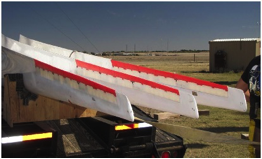
\includegraphics[width=.75\linewidth]{Figures/ch1Figures/fig1-4.png}
	\caption{Wind turbine blades with trailing edge flaps for active load control.\cite{berg2012}}
	\label{fig1-4}
\end{figure}

In LIDAR assisted control a LIDAR (Light Detection and Ranging) system is mounted on the nacelle of a turbine and used to scan the wind field as it approaches the wind turbine.  As illustrated in Figure \ref{fig1-5}, the LIDAR system is capable of measuring wind speed at several discrete distances upwind of the turbine.  These measurements are used to estimate the wind speed that the turbine will experience in the future.  The turbine controller can use these future wind speed estimates to respond preemptively to changes in wind speed and to counteract changes in aerodynamic loading as they occur. The primary disadvantage to LIDAR control is the prohibitive cost of the LIDAR equipment.  

\begin{figure}[htbp]
	\centering
		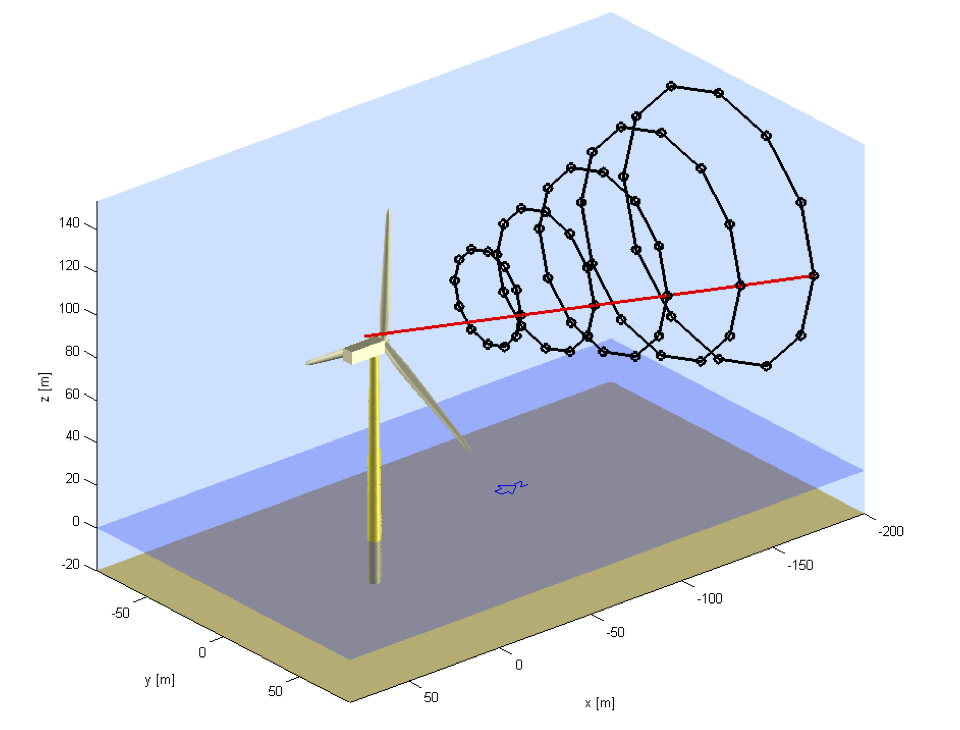
\includegraphics[width=.75\linewidth]{Figures/ch1Figures/fig1-5.png}
	\caption{Illustration of upwind LIDAR measurement distances.\cite{schlipf2011}}
	\label{fig1-5}
\end{figure}

%----------------------------------------------------------------------------------------
%	SECTION 4
%----------------------------------------------------------------------------------------

\section{Goals of This Research} 

This thesis seeks to improve wind turbine control by using information obtained from upwind turbines.  In particular, pre-existing sensors on upwind turbines will measure wind speed fluctuations and dynamic turbine behavior.  That information will then be used by the control system of a downwind turbine to anticipate wind speed fluctuations before they reach the downwind turbine.  This technique holds the potential to improve power production and/or decrease turbine loads by allowing the downwind turbine to react preemptively to changes in wind speed and track the optimum turbine conditions more closely.

Figure \ref{fig1-6} shows the steady state power curve for the NREL 5-MW turbine.  It represents the optimum power production at each wind speed.  If the wind blows at a constant speed for long enough, the control system will bring the turbine$'$s power production to a point on the blue line.  However, since rapid wind speed fluctuations are common, the turbine often deviates from this power curve during normal operation.  If the magnitude and/or time of these deviations can be reduced then the power curve can be tracked more closely and several potential benefits can be achieved.


\begin{figure}[htbp]
	\centering
		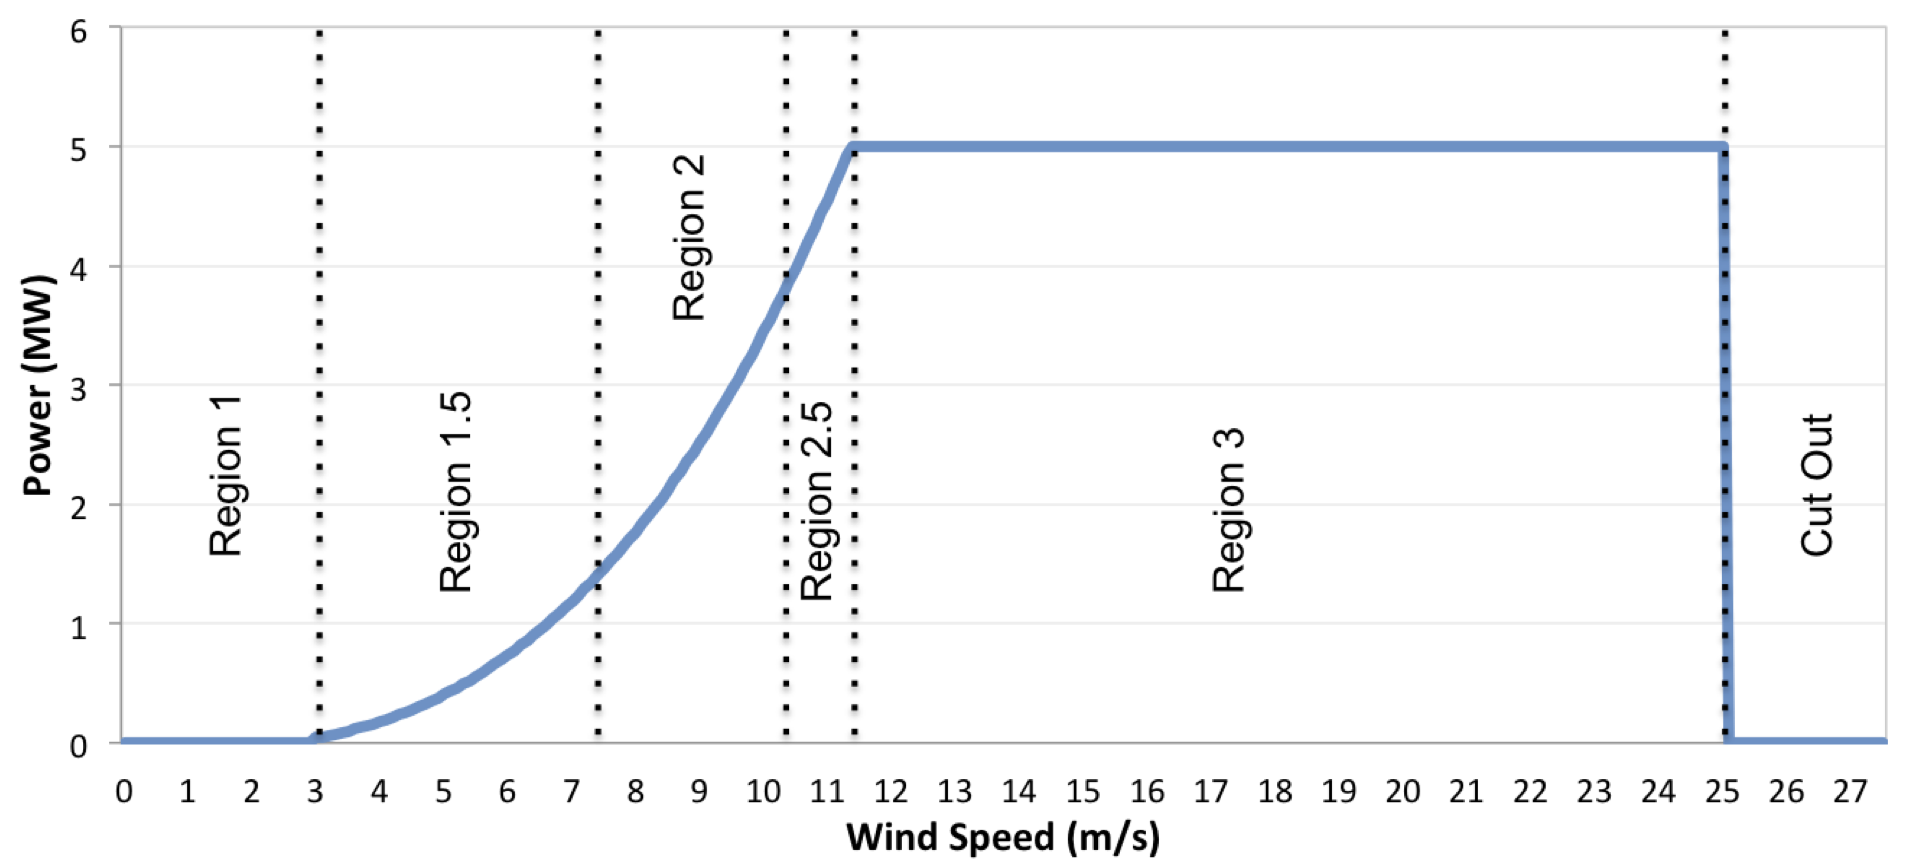
\includegraphics[width=\linewidth]{Figures/ch1Figures/fig1-6.png}
	\caption{Steady state behavior of the NREL 5-MW.\cite{jonkman2009}}
	\label{fig1-6}
\end{figure}

In region 2, deviations from the steady state power curve result in decreased aerodynamic efficiency and decreased power production.  By tracking the power curve more closely in this region the power production of the turbine can be increased.  In region 3, deviations from the steady state power curve cause higher loads on the mechanical components of the turbine and fluctuations in the power output of the turbine.  By tracking the power curve more closely the peak mechanical loads and fluctuation in power production can be reduced.

Reducing peak mechanical loads has several advantages.  It reduces wear and tear on the turbine$'$s mechanical components, thereby reducing the long-term repair and maintenance costs.  It can also lead to lower turbine-manufacturing costs or increased power production.  Reductions in manufacturing costs are achieved by designing and sizing the turbine components based on the reduced loads.  Alternately, increased power is achieved by “growing the rotor”.  Which means to increase the size of the turbine blades until the loading on the turbine components matches the original design loads.

Reducing the power fluctuations in region 3 can also be used to increase power production without any physical changes to the turbine.  In part, the rated power of a turbine is set by the limitations of the turbine$'$s power electronics.  If improvements in wind turbine control can reduce deviations from rated power then the turbine can safely operate at a higher rated power without fear of overloading the power electronics.  This technique is currently being used by General Electric with its WindBOOST control system. The WindBOOST control system update allows the GE 1.5 MW wind turbine to operate at a rated power of 1.6 MW without any changes to the turbine hardware. \cite{GE2009}



%----------------------------------------------------------------------------------------
%	SECTION 5
%----------------------------------------------------------------------------------------

\section{Dissertation Outline}

In the following sections ...
% Chapter Template

\chapter{Using a Wind Turbine as a Sensor} % Main chapter title

\label{Chapter2} % Change X to a consecutive number; for referencing this chapter elsewhere, use \ref{ChapterX}


%----------------------------------------------------------------------------------------
%	SECTION 1
%----------------------------------------------------------------------------------------

\section{Introduction}

When using a wind turbine as a sensor, the fundamental questions are: What should we measure, and how should we measure it? In this chapter several possible answers to those questions are investigated. To minimize the cost of the control system we will restrict ourselves to using sensors that are already present on a typical wind turbine. This chapter will first evaluate several methods for estimating wind speed, but will also investigate other potentially useful measurements.

There are two advantages to measuring wind speed.  First, both the steady state torque and steady state collective blade pitch are ultimately functions of the incoming wind speed (as shown in Figure \ref{fig2-1}).  Second, the wind speed provides an estimate of the speed at which turbulent eddies in the wind travel. As a result, the wind speed can be used to estimate how long it will take for the wind gusts observed by the upwind turbine to reach the downwind turbine. 


\begin{figure}[htbp]
	\centering
		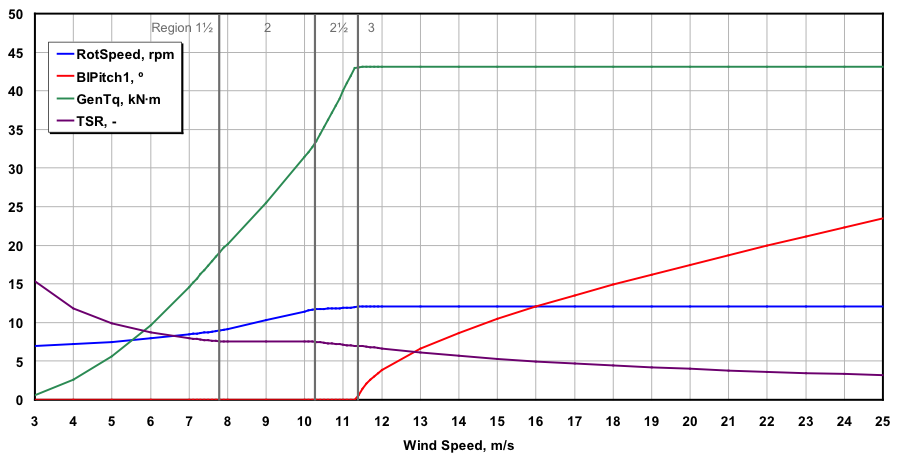
\includegraphics[width=\linewidth]{Figures/ch2Figures/fig2-1.png}
		
	\caption{Steady state behavior of the NREL 5-MW.\cite{jonkman2009}}
	\label{fig2-1}
\end{figure}

The following section will describe the generation of a simulation data set that is used to evaluate sensor techniques. The following three sections will discuss three methods for estimating the incoming wind speed of a turbine, nacelle top anemometer measurements, Turbine dynamics based estimation, and pressure measurement based estimation.  The final section of the chapter will discuss the viability of using blade pitch and generator speed as feed forward signals.



%----------------------------------------------------------------------------------------
%	SECTION 2
%----------------------------------------------------------------------------------------

\section{Data for evaluating sensor techniques} \label{section2-2}

The rest of this chapter discusses several wind turbine sensor scheme$'$s that could potentially be used for feed forward of downwind turbines. To gain insight into the performance of these scheme$'$s a series of simulations were conducted. The simulations were carried out in FAST (Fatigue, Aerodynamics, Structures, and Turbulence), using wind conditions simulated by TurbSim. FAST is a medium fidelity wind turbine simulation tool developed by NREL and Oregon State University. FAST models both the aerodynamics and structural dynamics of horizontal axis wind turbines, and has been independently validated and verified\cite{manjock2005}. TurbSim is a stochastic, full-field, turbulent-wind simulator. It uses a statistical model (as opposed to a physics based model) to numerically simulate a time series of three-component wind-speed vectors at points on a two-dimensional vertical rectangular grid (see Figure \ref{fig2-2}) \cite{jonkman2012}. All simulations described in this section assumed an NREL 5-MW turbine in great plains low level jet (GPLLJ) wind conditions.

\begin{figure}[htbp]
	\centering
		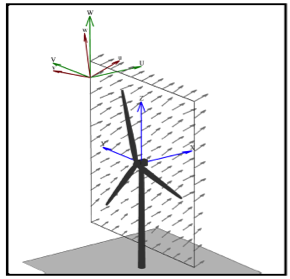
\includegraphics[width=.5\linewidth]{Figures/ch2Figures/fig2-2.png}
		
	\caption{Illustration of TurbSim flow field.\cite{jonkman2012}}
	\label{fig2-2}
\end{figure}

A variety of mean wind speeds were simulated to capture performance over the turbine$'$s whole operating range. Eleven (11) Mean wind speeds were simulated ranging from 4 m/s to 24 m/s in 2 m/s increments. At each wind speed 6 unique turbulent wind fields were generated using TurbSim. Each of these wind fields were used to drive a FAST simulation of the NREL 5-MW turbine. Each simulation was 10 minutes long. In total 66 10-minute simulations of a NREL 5-MW turbine in GPLLJ winds were performed.  Sample input files for the simulations can be found in appendix \ref{AppendixA}.





%----------------------------------------------------------------------------------------
%	SECTION 3
%----------------------------------------------------------------------------------------

\section{Wind speed estimate based on nacelle top \\
anemometer}

All utility scale wind turbines have nacelle-mounted anemometers. The wind speed measurements from the anemometer are used for purposes such as assessing wind turbine performance and forecasting future power production. The measurements from the anemometer are not used by conventional wind turbine control systems, but could potentially be used for wind turbine control.

In some ways, using a nacelle top anemometer is the simplest method to estimate incoming wind speed. The anemometer is designed to measure wind speed. It is located on top of the nacelle, which is near the center of the rotor$'$s swept area. The anemometer and data acquisition system are already in place on all commercial wind turbines. 

However, this method has several complications as well. The anemometer only measures wind speed for a very small portion of the flow field. On modern utility scale wind turbines, where rotors are often more than 100 meters in diameter, the anemometer reading may not be sufficient to accurately represent wind speed across the whole rotor. In addition, suitable anemometer data may not be readily available. For example, the data acquisition system on a Vestas V90 turbine does not provide the raw anemometer data. Instead it provides 10 minute average wind speeds that a proprietary filtering of the nacelle top anemometer data. For the sake of this investigation we will assume that the raw anemometer data can be obtained, perhaps with the help of the turbine manufacturer.

If suitable anemometer data is available, there may be difficulty obtaining an accurate wind speed measurement. Anemometer data  has high frequency noise and occasional false values. The anemometer could have errors due to poor calibration. In addition, the nacelle top location of the anemometer means it is measuring wind that has passed through the rotor plane. The simulation results shown in Figure \ref{fig2-3} were generated using SOWFA (Simulator fOr Wind Farm Applications), a simulation tool that will be discussed in Chapter \ref{Chapter5}. As Figure \ref{fig2-3} shows, wind in the nacelle area can be significantly affected by the rotor. For the sake of this investigation, we will assume the anemometer data can be processed to obtain an accurate measurement of the incoming wind speed at the center of the rotor.



\begin{figure}[htbp]
	\centering
		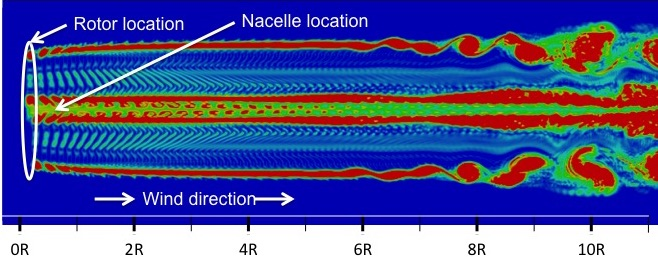
\includegraphics[width = \linewidth]{Figures/ch2Figures/fig2-3.jpg}
		
	\caption{Vorticity downstream of an NREL 5-MW rotor in uniform 11 m/s wind.}
	\label{fig2-3}
\end{figure}





%-----------------------------------
%	SUBSECTION 3-1
%-----------------------------------
\subsection{Feasibility}

The simulation dataset described in Section \ref{section2-2} was used to evaluate the feasibility of using a nacelle top anemometer to estimate incoming wind speed.  FAST does not simulate the nacelle top anemometer. However, if we make the assumptions stated in the previous two paragraphs we can treat true the incoming wind speed at the center of the rotor as a filtered and processed signal from the nacelle top anemometer. The true incoming wind speed at the rotor center can be extracted from the TurbSim flow field, and will be treated as the nacelle top anemometer measurement for the remainder of this discussion(Figure \ref{fig2-4}-a). The average wind speed passing through the rotor of the turbine can also be calculated from the TurbSim flow field (Figure  \ref{fig2-4}-b). By comparing these two values we get a feel for how well a nacelle top anemometer can represent the wind passing through the rotor of a utility scale turbine.

\begin{figure}[htbp]
	\centering
		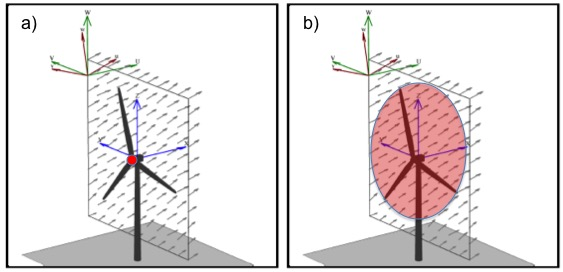
\includegraphics[width = \linewidth]{Figures/ch2Figures/fig2-4.jpg}
		
	\caption{Measurement locations for the rotor center wind speed and rotor average wind speed.}
	\label{fig2-4}
\end{figure}

Figure \ref{fig2-6} shows the wind speed at the anemometer as well as the average wind speed across the swept area of the rotor. The data shown in the figure is from the 13th simulation in the data set described above, but this data is typical of the other 65 simulations as well. At first glance the anemometer wind speed looks noisy compared to the rotor average wind speed. Upon closer examination (Figure \ref{fig2-7}) we see that both the anemometer and the rotor average wind speed have high frequency fluctuations. However, the high frequency fluctuations in the anemometer wind speed have a much larger magnitude. 

\begin{figure}[htbp]
	\centering
		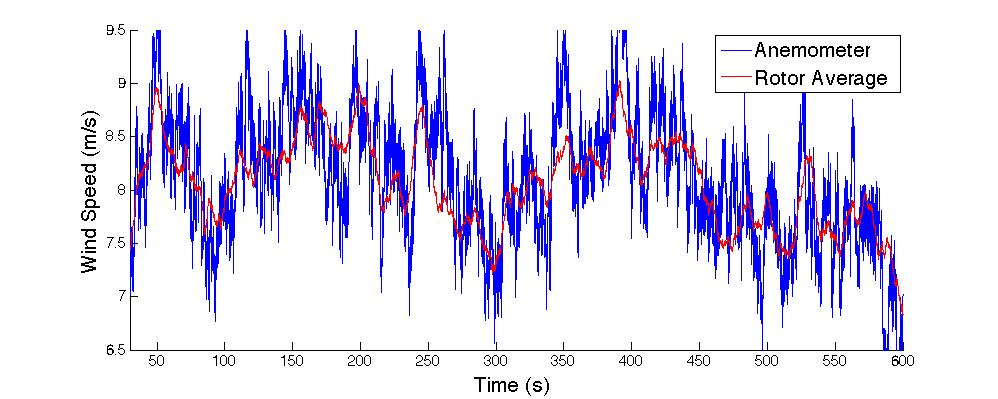
\includegraphics[width = \linewidth]{Figures/ch2Figures/fig2-6.jpg}
		
	\caption{Anemometer measurement and rotor average wind speed for simulation \#13 (8 m/s average wind speed).}
	\label{fig2-6}
\end{figure}


\begin{figure}[htbp]
	\centering
		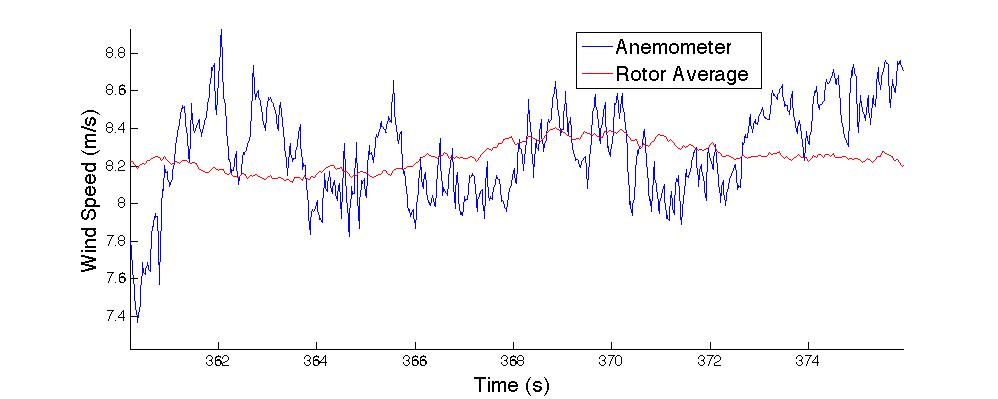
\includegraphics[width = \linewidth]{Figures/ch2Figures/fig2-7.jpg}
		
	\caption{Anemometer measurement and rotor average wind speed for simulation \#13 (8 m/s average wind speed).}
	\label{fig2-7}
\end{figure}

The magnitude of these high frequency fluctuations is not very important from a wind turbine control point of view. Because utility scale wind turbines are such large machines, it isn$'$t practical for the blade pitch and generator torque to track high frequency fluctuations in wind speed. In a typical utility scale turbine controller feedback signals are passed through a low pass filter before they are used for turbine control. To get a more meaningful comparison between anemometer wind speed and rotor average wind speed we should filter out the high frequency fluctuations.

Figure \ref{fig2-8} shows the anemometer wind speed and rotor average wind speed from simulation \#13 after they have been passed through a low pass filter. I chose to use a 4th order zero-phase filter with a 0.25 Hz cutoff frequency. A zero phase filter was chosen because it does not result in a delay of the filtered signal. A 0.25 Hz cutoff frequency was chosen because it is the corner frequency of the low pass filter used by the NREL 5-MW control system. 

\begin{figure}[htbp]
	\centering
		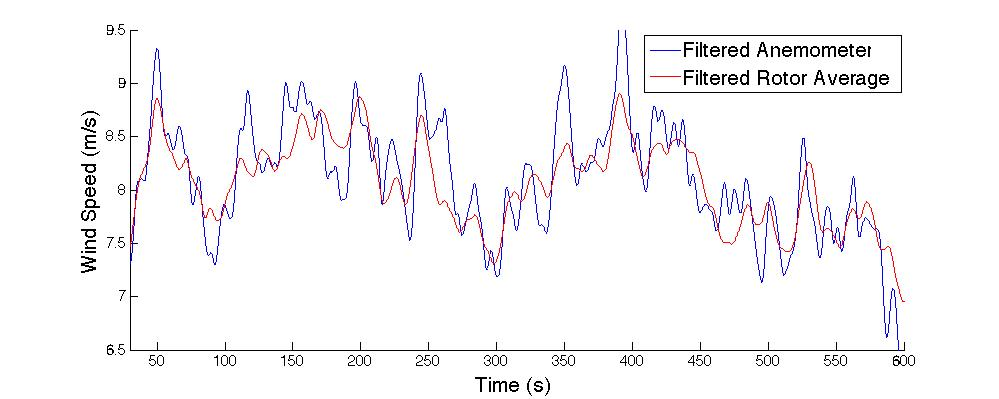
\includegraphics[width = \linewidth]{Figures/ch2Figures/fig2-8.jpg}
		
	\caption{Filtered anemometer and rotor average wind speed for simulation \#13.}
	\label{fig2-8}
\end{figure}

Figure \ref{fig2-9} shows the discrepancy between the filtered anemometer wind speed and the filtered rotor average wind speed for simulation \#13. For this run the magnitude of the discrepancy ranges from almost 0 to as much as 0.954 m/s, and the average magnitude of the discrepancy is 0.236 m/s. All 6 simulations run with an 8 m/s wind speed yield similar data, as can be seen in Figure \ref{fig2-10}. Between these 6 simulations we have 57 minutes of data. If we average the magnitude of the discrepancy over all the data points in these 6 simulations we find the discrepancy between the filtered anemometer wind speed and the filtered rotor average wind speed averages 0.272 m/s when the NREL 5-MW turbine is in 8 m/s GPLLJ wind conditions.

\begin{figure}[htbp]
	\centering
		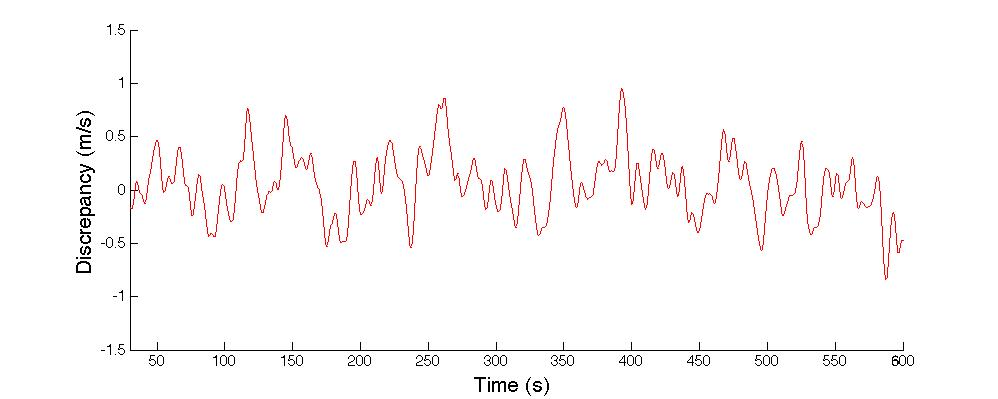
\includegraphics[width = \linewidth]{Figures/ch2Figures/fig2-9.jpg}
		
	\caption{Discrepancy between anemometer and rotor average wind speed for simulation \#13.}
	\label{fig2-9}
\end{figure}

\begin{figure}[htbp]
	\centering
		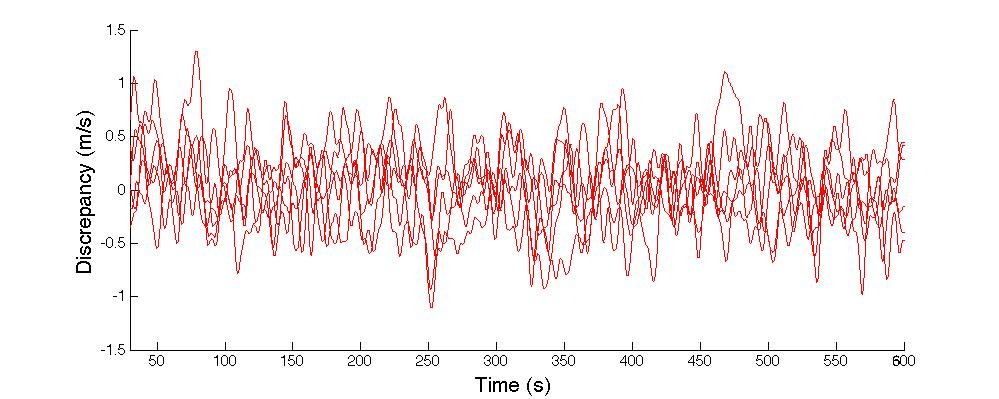
\includegraphics[trim = {.25cm 0 2.5cm 0}, clip, width = .95\linewidth]{Figures/ch2Figures/fig2-10.jpg}
		
	\caption{Discrepancy between anemometer and rotor average wind speed for all 8 m/s simulations.}
	\label{fig2-10}
\end{figure}


Repeating that process for all the mean wind speeds simulated in the data set yields Figure \ref{fig2-11} and Figure \ref{fig2-12}. Figure \ref{fig2-11} shows average magnitude of the discrepancy between in m/s, while Figure \ref{fig2-12} shows the same quantity expressed as a percentage the mean wind speed. Each \* on the plot represents an average over all 57 minutes of simulation data at the corresponding wind speed. Figure \ref{fig2-11} shows that the smallest average discrepancy is 0.269 m/s, which occurs at a mean wind speed of  6 m/s. When we examine the discrepancy as a percentage of the mean free stream wind speed  (Figure \ref{fig2-12}) we see that the average discrepancy is approximately 3\% of the mean wind speed over most of the operating range of the NREL 5-MW turbine, though the  average discrepancy is a larger percentage at low wind speeds.

\begin{figure}[htbp]
	\centering
		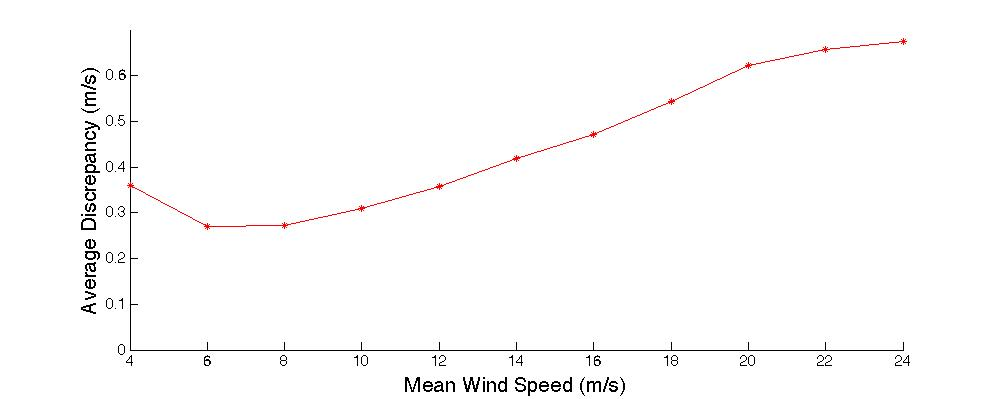
\includegraphics[width = \linewidth]{Figures/ch2Figures/fig2-11.jpg}
		
	\caption{Average magnitude of discrepancy as a function of simulation mean wind speed.}
	\label{fig2-11}
\end{figure}

\begin{figure}[htbp]
	\centering
		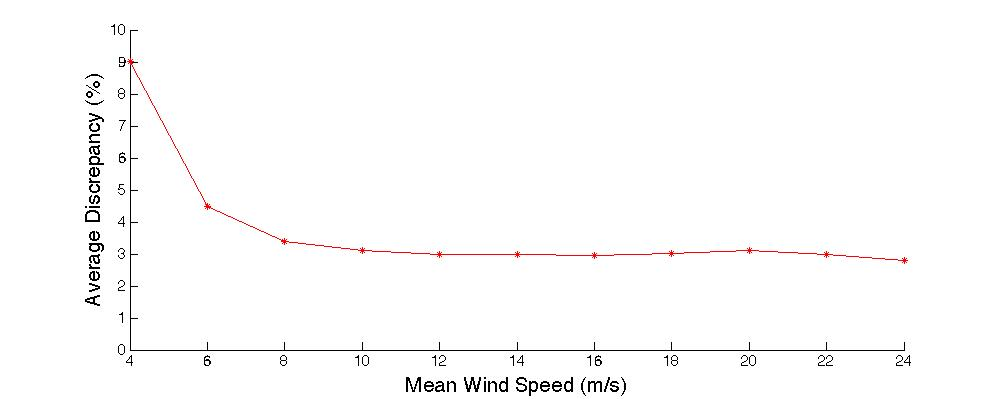
\includegraphics[width = \linewidth]{Figures/ch2Figures/fig2-12.jpg}
		
	\caption{Average magnitude of discrepancy as a function of simulation mean wind speed.}
	\label{fig2-12}
\end{figure}



%----------------------------------------------------------------------------------------
%	SECTION 4
%----------------------------------------------------------------------------------------

\section{Turbine Model Based Wind Speed Estimator} \label{section2-4} 

Incoming wind speed can also be estimated using an inverted model of the turbine.  First the generator speed, generator torque, and pitch angle are measured.  The inverted model is then used to determine the mean incoming wind speed that would cause the observed turbine operating conditions.  In effect, the turbine itself is used as a wind speed sensor. \cite{ostergaard2007,vanderhooft2004,schlipf2014}

We begin with a simplified model of the wind turbine in which the only degrees of freedom are the rotational speed of the rotor ($\Omega _{Rotor}$), the collective blade pitch ($\theta$), and the torque supplied by the generator ($T_{Gen}$).  The dynamics of the turbine are given by equation \ref{eq2-1}, where $I_{Drivetrain}$ is the low speed shaft equivalent inertia, $T_{Aero}$ is the aerodynamic torque on the rotor, and $N_{Gear}$ is the gear box ratio:

\begin{equation}
	\dot{\Omega }_{Rotor}I_{Drivetrain}=T_{Aero}-T_{Gen}N_{Gear} \label{eq2-1}
\end{equation}

Essentially, equation  \ref{eq2-1} says the rotational acceleration of the rotor multiplied by the effective inertia of the rotor is equal to the sum of the torques applied to the rotor. The low speed shaft equivalent inertia ( $I_{Drivetrain}$) is the rotational inertia of the rotor plus the apparent inertia due other components of the drivetrain. It can be calculated from the rotational inertias of the drivetrain components and the gearbox ratio ($N_{Gear}$). There are two torques applied to the rotor. The torque exerted by the generator is equal to the generator torque multiplied by the gearbox ratio. The aerodynamic torque exerted on the rotor by the incoming wind ($U$) is given by equation \ref{eq2-2}, where $\rho$ is is air density, $R$ is the rotor radius, $C_p$ is the coefficient of power, and $\lambda$ is the tip speed ratio:

\begin{equation}
	T_{Aero}=\frac{1}{2}\rho R^{3}\frac{C_{p}(\lambda,\theta)}{\lambda}U^{2} \label{eq2-2}
\end{equation}

The tip speed ratio $\lambda$ is the ratio between the speed of the turbine blade tips and the speed of the incoming wind. It can be calculated using equation \ref{eq2-3}. The coefficient of power $C_p$ is a non-linear function of both tip speed ratio and collective blade pitch angle. A method for determining $C_p$ will be discussed below

\begin{equation}
	\lambda=\frac{\Omega_{Rotor} R}{U} \label{eq2-3}
\end{equation}

Equation \ref{eq2-2} has four quantities that are not directly measurable: $T_{Aero}$, $C_p,$ $\lambda$, and $U$. If equation \ref{eq2-1} is used to substitute for $T_{Aero}$ equation \ref{eq2-2} becomes:

\begin{equation}
	\dot{\Omega }_{Rotor} I_{Drivetrain} + T_{Gen} N_{Gear} = \frac{1}{2} \rho R^3 \frac{C_p ( \lambda , \theta )}{\lambda} \left(\frac{\Omega_{Rotor} R}{\lambda}\right)^2   \label{eq2-4}
\end{equation}

Which can be re-arranged to yield equation \ref{eq2-5}. All the terms on the right side of equation \ref{eq2-5} are known or easily measured from sensors on the wind turbine. Therefore, equation \ref{eq2-5} can be used to calculate $C_p / \lambda^3$.

\begin{equation}
	 \frac{C_p ( \lambda, \theta)}{\lambda^3} = \frac{2 \dot{\Omega}_{Rotor} I_{Drivetrain} + 2 T_{Gen} N_{Gear}}{\rho R^5 \Omega^2_{Rotor}} \label{eq2-5}
\end{equation}


The coefficient of power $C_p$ is a non-linear function of both tip speed ratio and collective blade pitch angle. It isn’t possible to calculate $C_p$ exactly, but for a given tip speed ratio and collective blade pitch it is possible to estimate the $C_p$ of a turbine through simulation.  Figure \ref{fig2-13} illustrates how $C_p$ of the NREL 5-MW turbine varies with $\lambda$ and collective pitch angle. This plot was generated from a large number of simulations carried out with WTPerf \cite{platt2012}. Note that the maximum $C_p$ corresponds to a 0\degree collective pitch angle and a tip speed ratio of 7.55. The turbine operates near this point when using variable speed control in region 2. 

\begin{figure}[htbp]
	\centering
		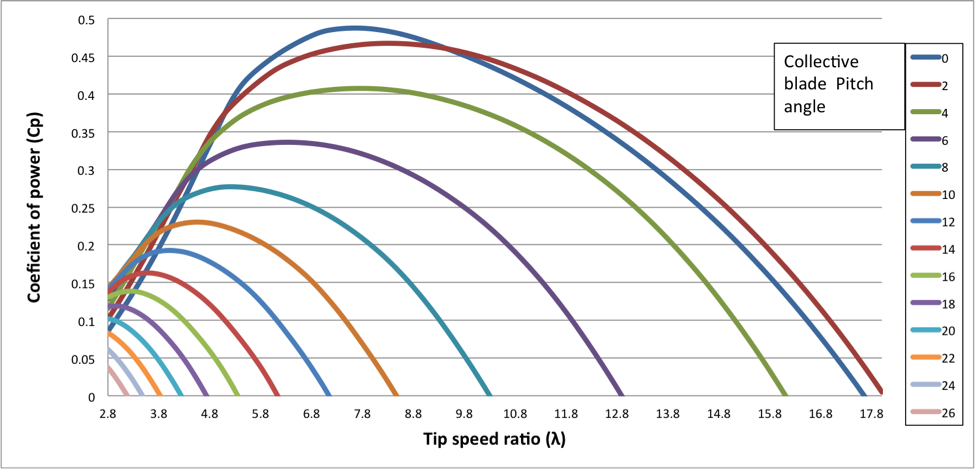
\includegraphics[width=\textwidth]{Figures/ch2Figures/fig2-13.png}
		
	\caption{$C_p$ dependence on $\lambda$ and collective blade pitch angle (\degree).}
	\label{fig2-13}
\end{figure}

The collective pitch angle is measured by turbine sensors, but both $C_p$ and $\lambda$ are unknown quantities that can not be directly measured or easily calculated. However, this problem can be fixed. If each $C_p$ value estimated by WTPerf is divided by the corresponding $\lambda$ cubed we get a relationship between $C_p\lambda^3, \lambda$, and collective pitch angle. Figure \ref{fig2-14}  illustrates how $C_p / \lambda^3$ of the NREL 5-MW turbine varies with $\lambda$ and collective pitch angle. 

\begin{figure}[htbp]
	\centering
		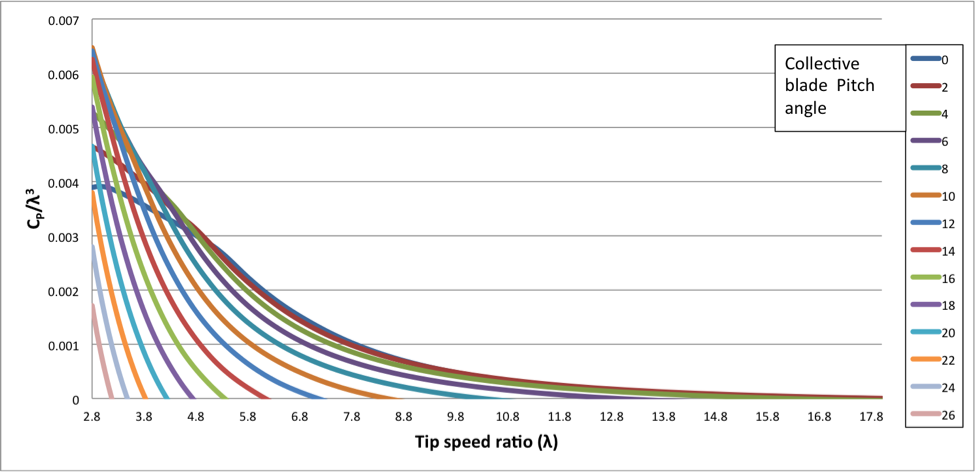
\includegraphics[width=\textwidth]{Figures/ch2Figures/fig2-14.png}
		
	\caption{$C_p / \lambda^3$ dependence on $\lambda$ and collective blade pitch.}
	\label{fig2-14}
\end{figure}

The incoming wind speed can now be estimated. First the collective pitch angle is measured and $C_p / \lambda^3$ is calculated using equation \ref{eq2-5}. $\lambda$ is then estimated by interpolating between the WTPerf simulation data points illustrated in Figure \ref{fig2-14}. Finally, $\lambda$ is converted to incoming wind speed ($U$) using equation \ref{eq2-3}. Matlab codes carrying out these calculations can be found in Appendix \ref{AppendixA}.


%-----------------------------------
%	SUBSECTION 4-1
%-----------------------------------
\subsection{Feasibility} \label{section2-4-1} 

The feasibility of using a wind turbine model based wind speed estimator was evaluated using similar methods to those used to evaluate the feasibility of using a nacelle top anemometer. We begin by comparing the average wind speed passing through the rotor of the turbine (calculated from the TurbSim flow field) to the wind speed estimated by the model based wind speed estimator.  This gives us a feel for how well the estimator represents the wind passing through the rotor of a utility scale turbine.

The data in Figure \ref{fig2-15} is from the 13th simulation in the data set described above (the same simulation shown in Figure \ref{fig2-6}), but this data is typical of the other 65 simulations as well. The figure shows that the wind speed estimator is “noisier” than the rotor average wind speed. In this way it$'$s similar to the nacelle anemometer measurements shown in Figure \ref{fig2-6} and Figure \ref{fig2-15} we see that high frequency fluctuations in the wind speed estimator are smaller than the high frequency fluctuations in the anemometer measurements. 

\begin{figure}[htbp]
	\centering
		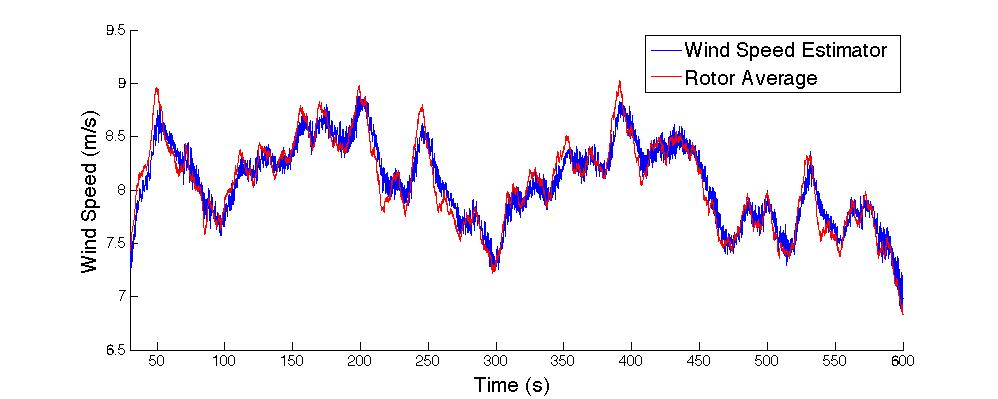
\includegraphics[width = \linewidth]{Figures/ch2Figures/fig2-15.jpg}
		
	\caption{Wind speed estimate and rotor average wind speed for simulation \#13.}
	\label{fig2-15}
\end{figure}


Filtering the data to remove the high frequency fluctuations yields Figure \ref{fig2-16}. The wind speed estimator doesn$'$t match the rotor average wind speed perfectly, but a comparison between Figure \ref{fig2-8} and Figure \ref{fig2-16} shows that the wind speed estimator does a much better job than the nacelle top anemometer. This conclusion is reinforced by comparing Figure \ref{fig2-9} to Figure \ref{fig2-17}.

\begin{figure}[htbp]
	\centering
		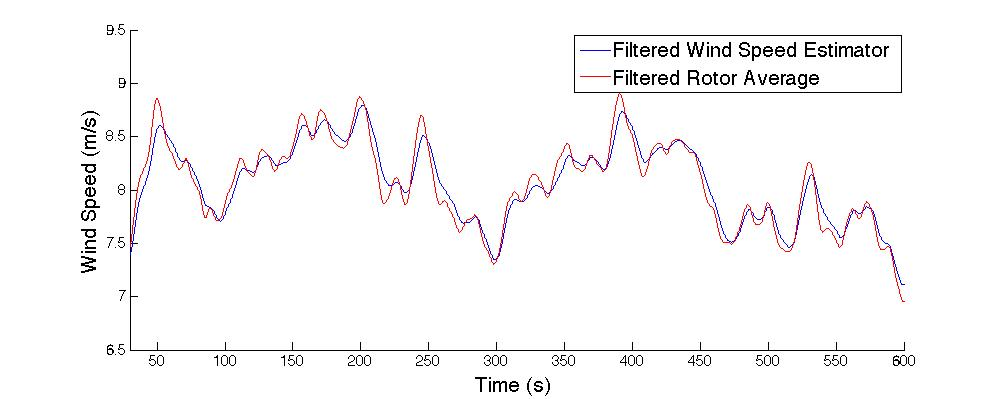
\includegraphics[width = \linewidth]{Figures/ch2Figures/fig2-16.jpg}
		
	\caption{Filtered wind speed estimate and rotor average wind speed for simulation \#13.}
	\label{fig2-16}
\end{figure}



\begin{figure}[htbp]
	\centering
		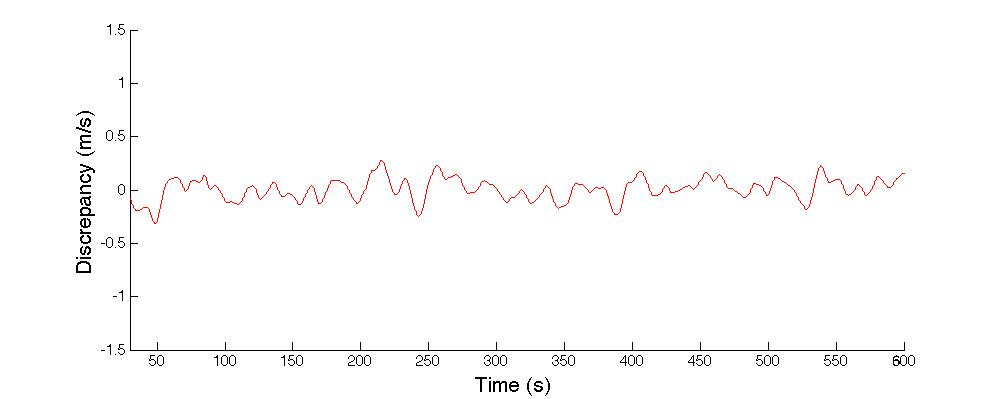
\includegraphics[width = \linewidth]{Figures/ch2Figures/fig2-17.jpg}
		
	\caption{Discrepancy between wind speed estimate and rotor average wind speed for simulation \#13.}
	\label{fig2-17}
\end{figure}

The data shown in Figures \ref{fig2-15}-\ref{fig2-17} are from a single simulation, but the data and the conclusions drawn from it are typical of all the simulation data examined. The wind sped estimator performed significantly better than the nacelle top anemometer. If we analyze the wind speed estimator data for all 66 simulations using the same process used to generate Figure \ref{fig2-11} and Figure \ref{fig2-12} we can get an idea of how much better the wind speed estimator performs. Figure \ref{fig2-18} and Figure \ref{fig2-19} compare the average discrepancy between the wind speed estimator and the rotor average wind speed to the average discrepancy between the nacelle top anemometer and the average wind speed. It can be seen from these figures that the wind speed estimator outperforms the anemometer across the entire operating range of the turbine. 


\begin{figure}[htbp]
	\centering
		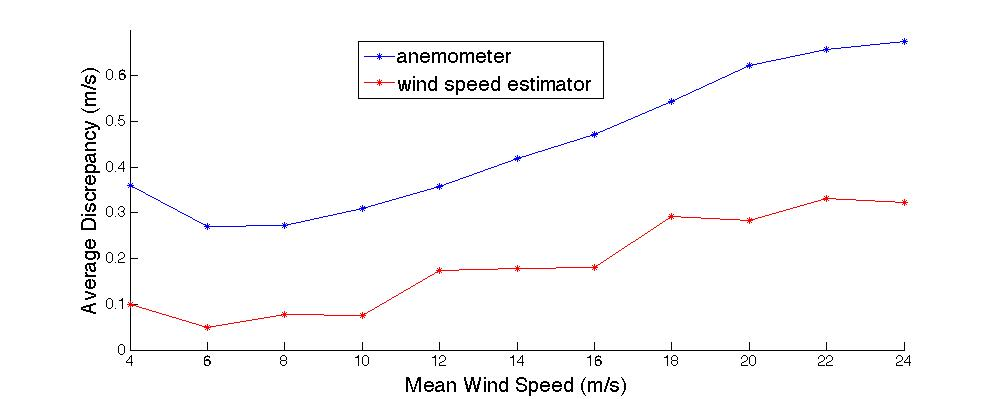
\includegraphics[width = \linewidth]{Figures/ch2Figures/fig2-18.jpg}
		
	\caption{Average magnitude of discrepancy as a function of simulation mean wind speed.}
	\label{fig2-18}
\end{figure}



\begin{figure}[htbp]
	\centering
		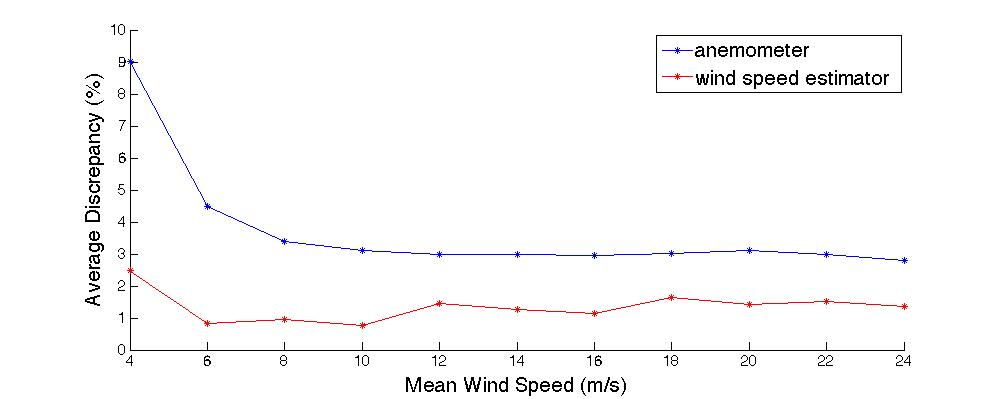
\includegraphics[width = \linewidth]{Figures/ch2Figures/fig2-19.jpg}
		
	\caption{Average magnitude of discrepancy as a function of simulation mean wind speed.}
	\label{fig2-19}
\end{figure}


%-----------------------------------
%	SUBSECTION 4-2
%-----------------------------------
\subsection{Effect of rotor yaw misalignment}\label{section2-4-2} 

The simulations analyzed in the previous sections assume the turbine is pointed directly into the wind. However, in normal turbine operation there is often some misalignment between the wind direction and the pointing direction, or yaw, of the turbine. It is possible to design a turbine that is stable in yaw and will point itself into the wind without the help of a control system or actuators, but in practice this passive control technique is only used for very small turbines. Modern utility scale turbines use active yaw control \cite{burton2011}.

The yaw control on a typical utility scale turbine uses a dead band controller with a nacelle mounted wind vane as a sensor and a nacelle yaw motor as an actuator \cite{burton2011}. In this control scheme the signal from the nacelle mounted wind vane is heavily averaged to reduce the effect of small brief changes in wind direction and to reduce the effect of the turbulence generated by the turbine rotor. That averaged wind direction is then treated as an estimate of the wind direction. The dead band controller compares the wind direction estimate to the current yaw of the turbine. If the misalignment is smaller than a pre-defined limit the controller does nothing, but if the misalignment exceeds the limit the controller engages the yaw motor and yaws the turbine into alignment with the wind. Since the NREL 5-MW turbine does not define a yaw control system, we will assume our turbine uses dead band control.

The amount of misalignment allowed by the dead band yaw controller will vary from one turbine to another. To evaluate the effect of yaw misalignment on wind speed estimation misalignments of 5\degree, 10\degree, 15\degree, and 20\degree were simulated. For each of these yaw misalignments the 66 test cases described above were simulated.

Figure \ref{fig2-20} shows the effect of rotor misalignment on wind speed estimation for simulation case \#13. As misalignment angle increases the wind speed estimator underestimates wind speed. For 5\degree and 10\degree misalignments this effect appears small, but the effect is much larger for 15\degree and 20\degree misalignments. It$'$s worth noting that the shapes of the wind speed estimate curves do not change much with increasing rotor misalignment. The misalignment primarily affects the magnitude of the wind speed estimates. 


\begin{figure}[htbp]
	\centering
		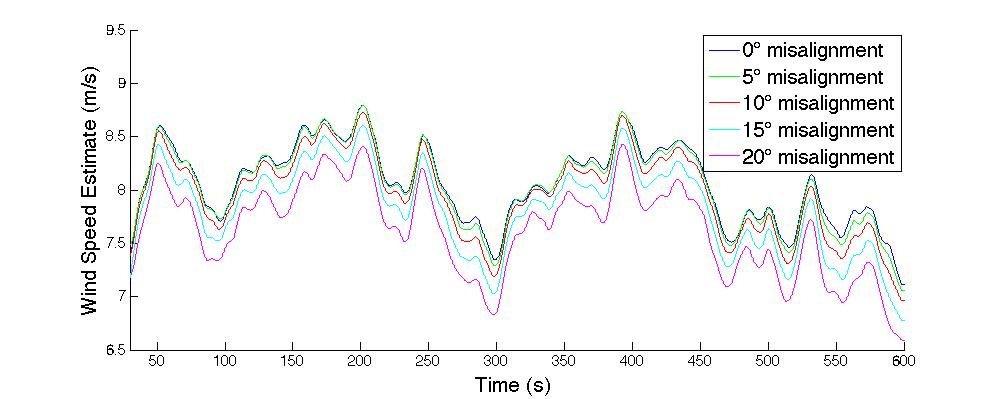
\includegraphics[width = \linewidth]{Figures/ch2Figures/fig2-20.jpg}
		
	\caption{Effect of rotor misalignment on wind speed estimate for simulation \#13.}
	\label{fig2-20}
\end{figure}

Though the data shown in Figure \ref{fig2-20} is from a single simulation case the conclusions drawn from it are typical of all simulation data that was examined. If we analyze the wind speed estimator data for all simulations cases using the same process used to generate Figure \ref{fig2-12} we can get an idea of how rotor misalignment affects wind speed estimation error. As we saw in Figure \ref{fig2-20} a misalignment of 5\degree or 10\degree causes only a small increase in the discrepancy between estimated wind speed and average rotor wind speed. Larger misalignments cause significantly larger discrepancies. It is worth noting only the 20\degree misalignment performs worse than the nacelle top anemometer (Figure \ref{fig2-12}).

\begin{figure}[htbp]
	\centering
		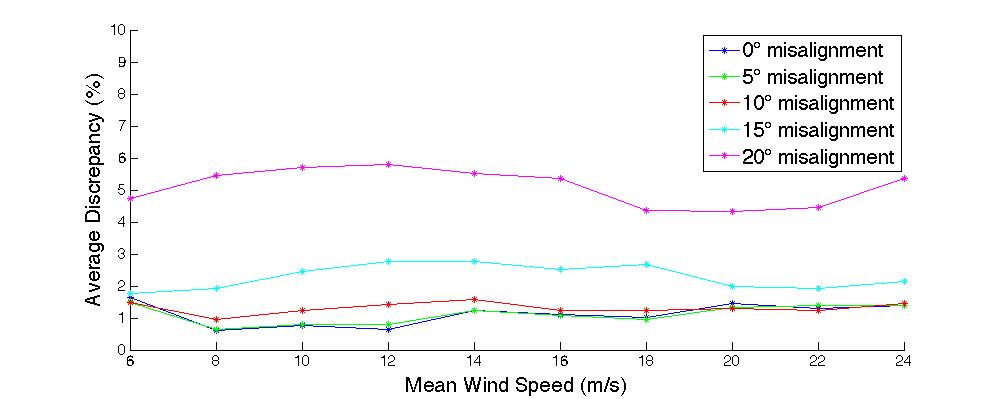
\includegraphics[width = \linewidth]{Figures/ch2Figures/fig2-21.jpg}
		
	\caption{Effect of misalignment on average magnitude of wind speed estimate discrepancy.}
	\label{fig2-21}
\end{figure}


It should not be surprising that a misaligned rotor underestimates wind speed. Our wind speed estimator is based on a simplified model of turbine rotor dynamics. Since wind parallel to the rotor plane does not exert an aerodynamic torque on the rotor our estimator does not measure that component of the wind. Essentially, our wind speed estimator is designed to measure the component of the wind that is perpendicular to the rotor plane. As Figure \ref{fig2-22} shows, the apparent wind seen by the wind speed estimator is equal to the actual wind multiplied by the cosine of the misalignment angle.

\begin{figure}[htbp]
	\centering
		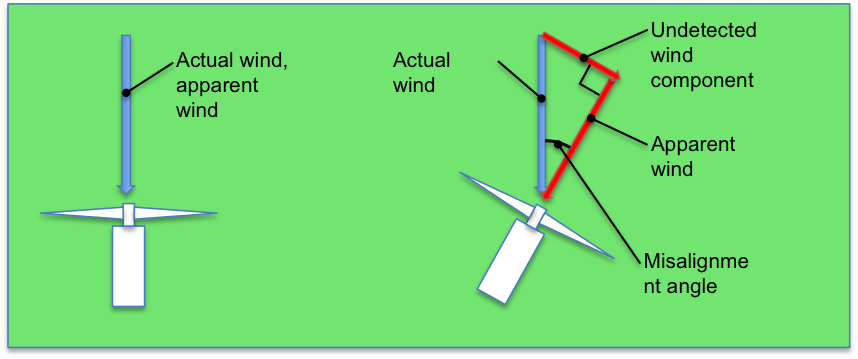
\includegraphics[width=\textwidth]{Figures/ch2Figures/fig2-22.png}
		
	\caption{Effect of rotor misalignment on apparent wind.}
	\label{fig2-22}
\end{figure}

If the misalignment angle is known it can be used to compensate for the difference between the apparent wind seen by the estimator and the actual wind. If the wind speed estimates shown in Figure \ref{fig2-20} are divided by the cosine of the misalignment angle it yields Figure \ref{fig2-23}. As the figure shows, the effect of misalignment on wind speed estimation has been greatly reduced. 


\begin{figure}[htbp]
	\centering
	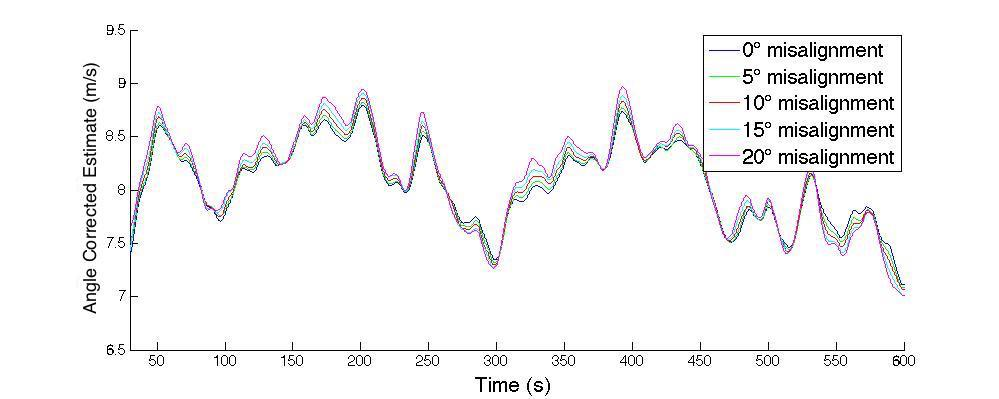
\includegraphics[width = \linewidth]{Figures/ch2Figures/fig2-23.jpg}
		
	\caption{Angle corrected wind speed estimates for simulation \#13.}
	\label{fig2-23}
\end{figure}


Figure \ref{fig2-24} shows the average discrepancy between misalignment-compensated wind speed estimates and rotor average wind speed. The misaligned simulations generally show more discrepancy than the perfectly aligned simulations. However, comparing Figure \ref{fig2-21} to Figure \ref{fig2-24} shows that misalignment compensation greatly reduces the discrepancy. In the 20\degree misalignment simulations the average discrepancy is reduced 60-75 \% by angle compensation.


\begin{figure}[htbp]
	\centering
		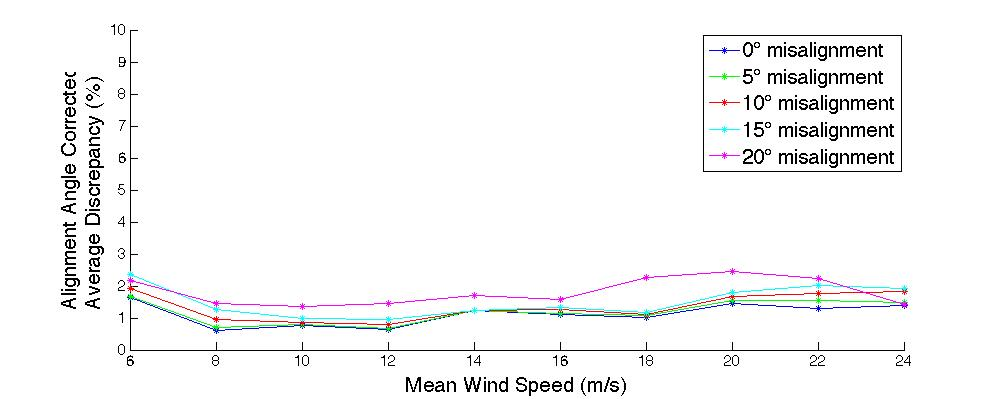
\includegraphics[width = \linewidth]{Figures/ch2Figures/fig2-24.jpg}
		
	\caption{Average magnitude of discrepancy in angle corrected wind speed estimates.}
	\label{fig2-24}
\end{figure}


Though the misalignment angle will not be perfectly known, an estimate of the misalignment angle will be available and can be used for compensation. As stated earlier in this section, the dead band yaw controller continuously estimates the misalignment angle but doesn$'$t act unless the misalignment exceeds a pre-defined limit. 

Yaw misalignment does have an effect on turbine model based wind speed estimation, but it does not appear that it will be a significant hindrance to using turbine model based wind speed estimation. Misalignments less than 10\degree only have a minor effect on performance. Larger misalignments do have a significant effect on performance, but it should be possible to reduce the effect by using misalignment angle compensation.





%----------------------------------------------------------------------------------------
%	SECTION 5
%----------------------------------------------------------------------------------------

\section{Convection speed estimation} \label{section2-5}

The previous sections have discussed instantaneous wind speed estimation. These wind speed estimates can be used to observe how the wind speed is fluctuating as it passes through a wind turbine rotor. However, knowledge of how the wind speed is fluctuating is not sufficient information for feed forward control of downwind turbines. We must also know when these wind speed fluctuations will reach the downwind turbine. The time required for the wind speed fluctuations to pass from the upwind turbine to the downwind turbine can be calculated with the simple equation $t = D/U_{conv}$, where $D$ is the downwind distance between the turbines and $U_{conv}$ is the convection speed. The convection speed is the rate at which wind speed fluctuations propagate downwind. This section will discuss using a wind turbine to estimate the convection speed.

If we assume Taylor's frozen turbulence hypothesis we can estimate the convection speed based on wind speed measurements taken at a single location. In this secion the convection speed will be estimated using the turbine model based wind speed estimates discussed in Section \ref{section2-4}. Taylor said ``If the speed of the air stream which carries the eddies is very much greater than the turbulence speed, one may assume that the sequence of changes in u at a fixed point are simply due to the passage of an unchanging pattern of turbulent motion over the point.'' \cite{taylor1938} In other words, the wind experienced by a point down wind of our sensor will be the same as the wind experienced by the sensor but it will be delayed by a time $t_D = (distance)/(U_{conv})$. It follows from Taylor's hypothesis that the convection speed of the turbulent fluctuations is equal to the local mean speed ($U_{mean}$). 

There is much research into the validity and limitations of Taylr's frozen turbulence hypothesis for estimating the convection speed. \cite{dennis2008,goldschmidt1981,delalamo2009,atkinson2015} Though research shows that the convection speed is not always equal to the mean speed they are frequently assumed to be equal in turbulent flow research. $U_{conv} = U_{mean}$ will be assumed for the remainder of this section. A more accurate estimate of the convection speed could be generated using more than one wind speed measurement location. For example, we could measure the time it took a gust of wind to travel between two turbines. However, this technique can not be used with the data set described in Section \ref{section2-2} because FAST only simulates a single turbine.

For the data set described in Section \ref{section2-2} the mean speed ($U_{mean}$) is known. $U_{mean}$ is one of the TurbSim input parameters used to generate the data set. As shown in equation \ref{eq2-6} we can consider the wind passing through the turbine rotor to be a combination of the underlying mean wind sped ($U_{mean}$) and the wind speed fluctuations due to turbulence ($U_{turb}$). If we average the hub height wind speed over a long enough time the wind speed fluctuations due to turbulence will cancel out and we'll be left with the mean wind speed. 


\begin{equation}
	 U =  U_{mean} +U_{turb}  \label{eq2-6}
\end{equation}

Figure \ref{fig2-25} shows the wind speed estimate, the sixty second average wind speed, and the true mean wind speed for simulation \#13. The wind speed estimate is generated using the method described in section \ref{section2-4}. 60 second average values are generated by averaging 60 seconds of wind speed estimate data (from 30 seconds before to 30 seconds after the time of interest). The true mean wind speed is known and was specified as an input when simulating the incoming wind. There are two things worth noting in Figure \ref{fig2-25}. First, there are significant discrepancies between the 60 second average wind speed and the known mean wind speed of 8 m/s. At 182 seconds there is a 0.587 m/s, or 7.3\%,  discrepancy between the 60 second average wind speed and the true mean wind speed. Also, the 60 second average wind speed out performs the wind speed estimator when it comes to estimating the true mean wind speed. Both the maximum and average discrepancy are lower for the 60 second average wind speed. 

\begin{figure}[htbp]
	\centering
		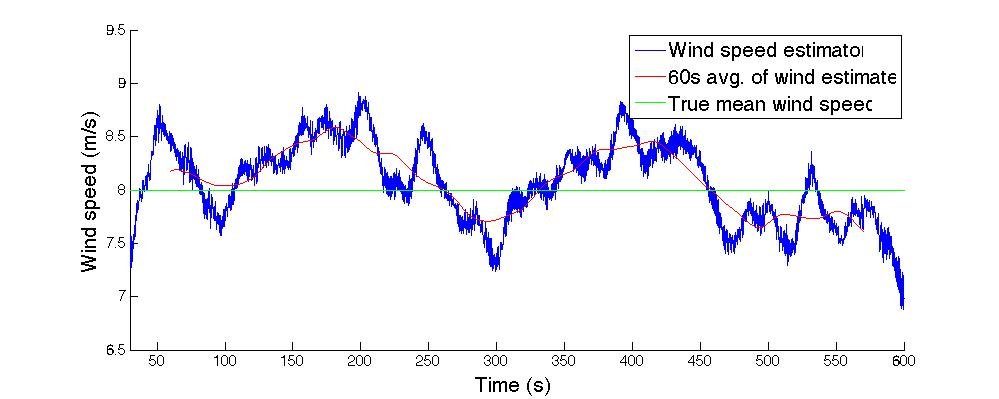
\includegraphics[width = \linewidth]{Figures/ch2Figures/fig2-25.jpg}
		
	\caption{Estimating $U_{mean}$ using a 60 s average of wind speed estimates for simulation \#13.}
	\label{fig2-25}
\end{figure}

By analyzing all of the test cases in our data set with a variety of averaging times we can generate Figures \ref{fig2-25} and \ref{fig2-26}. These figures show the maximum and average discrepancies between the various averaged wind speed estimates and the known true mean wind speeds. In Figure \ref{fig2-25} we see that longer average times result in smaller mean discrepancies between the average wind speed estimate and the true mean wind speed. This is expected. Longer averaging times would likely perform even better, but 570 seconds was the longest averaging time we could use with the current data set. The highest mean discrepancies (as a \% of the true mean wind speed) are at low wind speeds. For some wind speeds (16 m/s - 22 m/s) Figure \ref{fig2-25} seems to show diminishing improvement for averaging times over 240 s. However, for the rest of the wind speeds Figure \ref{fig2-25} does not seem to show a clear point of diminishing returns.

Figure \ref{fig2-26} largely shows the same trends that we see in Figure \ref{fig2-25}, but the trends are a little less clear. Figure \ref{fig2-26} shows a few unexpected results. For example, in 18 m/s wind Figure \ref{fig2-26} an averaging time of 240 s gives a larger maximum discrepancy than any of the shorter or longer averaging times. I suspect that if we analyzed a lot more data some of these unexpected results would no longer be present.



\begin{figure}[htbp]
	\centering
		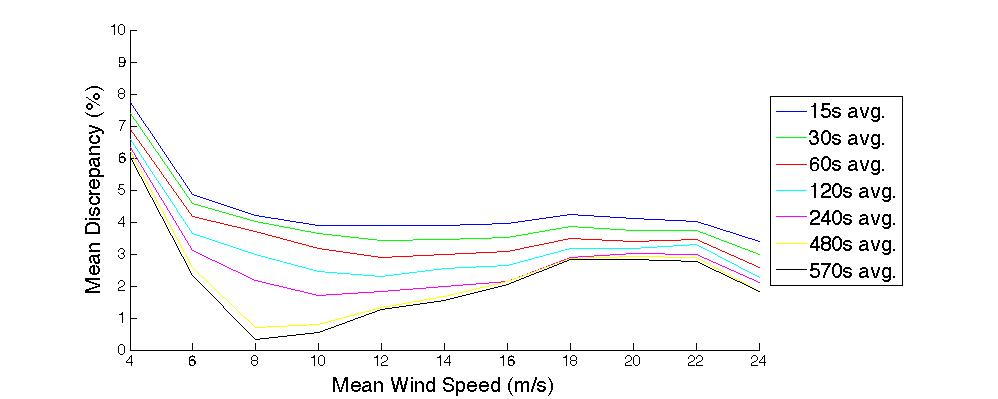
\includegraphics[width = \linewidth]{Figures/ch2Figures/fig2-26.jpg}
		
	\caption{Mean discrepency between true $U_{mean}$ and estimated $U_{mean}$ for a variety of averaging times.}
	\label{fig2-26}
\end{figure}

\begin{figure}[htbp]
	\centering
		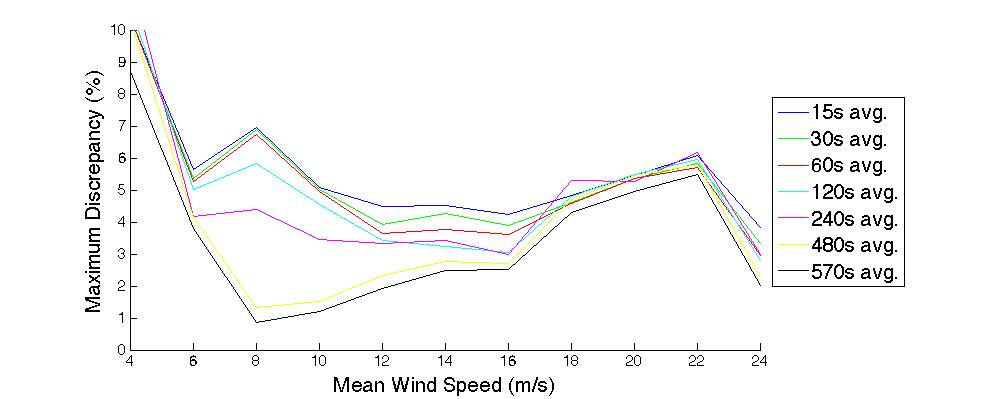
\includegraphics[width = \linewidth]{Figures/ch2Figures/fig2-27.jpg}
		
	\caption{Max discrepency between true $U_{mean}$ and estimated $U_{mean}$ for a variety of averaging times.}
	\label{fig2-27}
\end{figure}

Though Figures  \ref{fig2-25} and \ref{fig2-26} imply that the averaging time should be as long as possible, there is a practical reasons why a very long averaging time would be undesireable. When we simulate wind fields using TurbSim the mean wind speed remains constant, but research has shown that in real world conditions the mean wind speed does not remian constant indefinitely. In real world conditions the mean wind speed may be slowly changing \cite{vanderhoven1957}. If the mean wind speed is changing, we can minimize the impact on our wind speed averaging by keeping the averaging time short and by centering the averaging window on the time of interest. If we choose to center our averaging window on the time of interest, our averaging time is further constrained by the amount of time it will take wind speed fluctuations to propagate from the upwind turbine to the downwind turbine. For example, if the mean wind speed is 20 m/s and the downwind turbine is 1260 m (10$\times$ the NREL 5-MW rotor diameter) behind the upwind turbine, it will take about 63 seconds for the wind speed fluctuations to travel from the upwind turbine to the downwind turbine. In that scenario, the averaging time must be less than 126 seconds.

%-----------------------------------
%	SUBSECTION 5-1
%-----------------------------------
\subsection{A few thoughts on the limitations of Taylor's Frozen Turbulence Hypothesis}
Though Taylor$'$s hypothesis is often invoked in investigations of atmospheric turbulence, experimental results have shown that it is not universally accurate.  In particular, Taylor$'$s hypothesis is more accurate over short distances than over long distances and it is more accurate for low frequency wind speed fluctuations than high frequency fluctuations. \cite{higgins2012, schlipf2010}

%----------------------------------------------------------------------------------------
%	SECTION 6
%----------------------------------------------------------------------------------------

\section{Summary and Conclusions} \label{section2-5}
% Chapter Template

\chapter{Feed forward optimum pitch control.} % Main chapter title

\label{Chapter3} % Change X to a consecutive number; for referencing this chapter elsewhere, use \ref{ChapterX}


%----------------------------------------------------------------------------------------
%	SECTION 1
%----------------------------------------------------------------------------------------

\section{Introduction} \label{section3-1}
As discussed in Section \ref{section1-2}, the closed loop control system of a typical utility scale wind turbine manipulates generator torque and collective blade pitch in order to control the power generation and rotor speed of the turbine. At low and medium wind speeds the blade pitch remains fixed at 0$^\circ$ while generator torque is manipulated to achieve the rotor speed that maximizes electricity generation. At high wind speeds the collective blade pitch is manipulated to manage loading on the wind turbine as well as to maintain constant rotor speed and power generation. For a given wind speed there is a desired rotor speed ($\Omega_{Rotor}$), collective blade pitch ($\theta$), and generator torque ($T_{Gen}$). Figure \ref{fig3-1} shows these desired values for the NREL 5-MW turbine. If the wind remined constant the control system of the NREL 5-MW turbine would bring $\Omega_{Rotor}, \theta, and T_{Gen}$ to the values shown in figure \ref{fig3-1} and maintain those desired conditions. However, since wind speeds often fluctuate (as shown in figure \ref{fig3-2}) and utility scale turbines are large mechanical devices that are unable to instantaneously adjust to changes in wind speed, turbines are frequently chasing the desired conditions instead of operating at the desired conditions.

\begin{figure}[htbp]
	\centering
		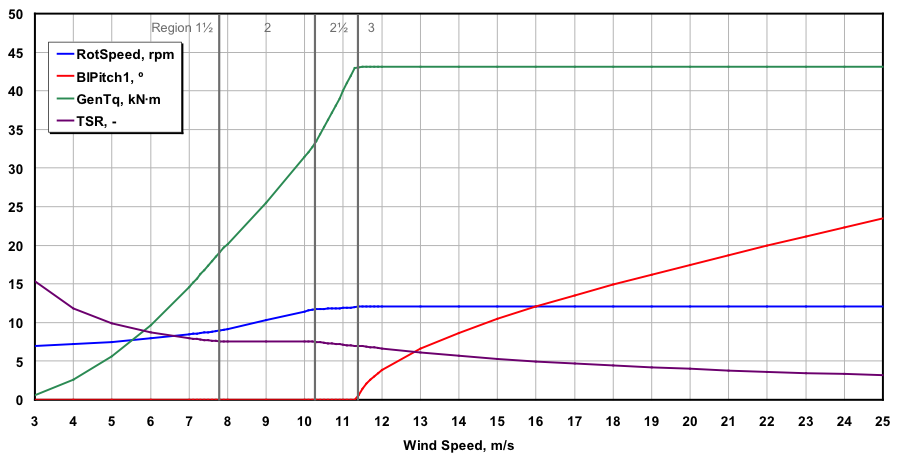
\includegraphics[width=\linewidth]{Figures/ch2Figures/fig2-1.png}
		
	\caption{Steady state behavior of the NREL 5-MW.\cite{jonkman2009}}
	\label{fig3-1}
\end{figure}

\begin{figure}[htbp]
	\centering
		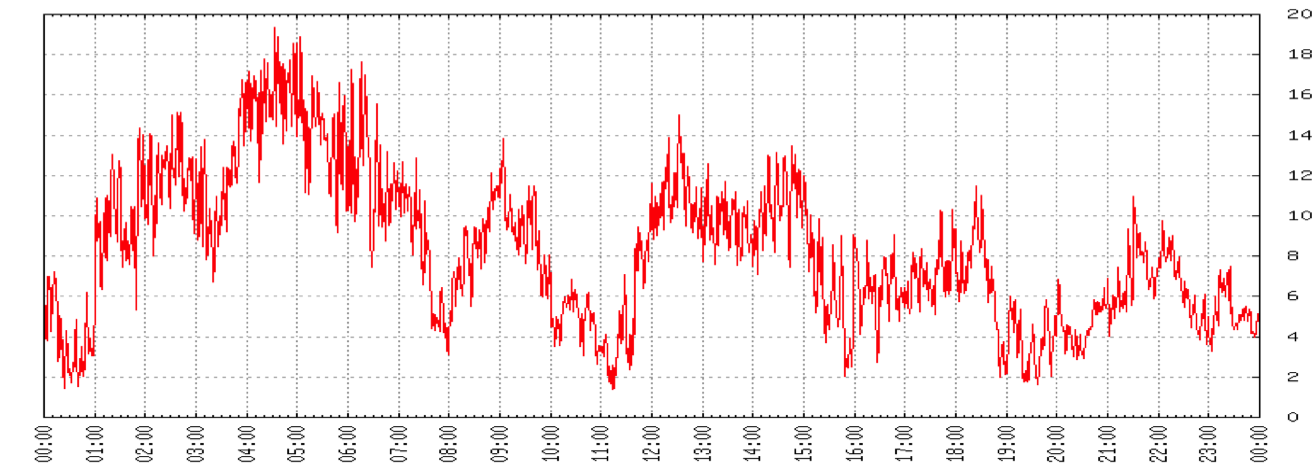
\includegraphics[width=\linewidth]{Figures/ch3Figures/fig3-2.png}
		
	\caption{An example of wind speed fluctuations over 24 hours.\cite{NWTC2013}}
	\label{fig3-2}
\end{figure}

Figures  \ref{fig3-3} and  \ref{fig3-4} illustrate the transient response of the NREL 5-MW turbine when subjected to sudden changes in wind speed. In both cases FAST has been used to model a NREL 5-MW turbine with the baseline controller defined in \cite{jonkman2009}. Figure \ref{fig3-3} illustrates turbine behavior in region 2, wind speeds between 7.8 m/s and 10.3 m/s, while Figure \ref{fig3-4} illustrates turbine behavior in region 3, wind speeds between 11.4 m/s and 25 m/s.  Each figure shows wind speed, “Actual” and “Optimal” power, generator torque, and blade pitch. “Actual” power is the power generated by the turbine. “Optimal” power is the desired steady state power generation for the current wind speed (based on the NREL 5-MW power curve shown in Figure \ref{fig1-6}). Generator torque and blade pitch are the two actuators used to control turbine performance. 

In Figure \ref{fig3-3} the turbine is subjected to a uniform incoming wind that changes between 8 m/s and 10 m/s every 20 seconds. These wind speeds are in region two, where optimal power production corresponds to the maximum aerodynamic efficiency of the turbine. Note that the turbine takes approximately 20 seconds to reach optimal generation after each change in wind speed. This corresponds to a reduction in efficiency.  The optimal power curve generates 0.6\% more power (15.6 kW on average) than the actual power curve. In this case turbine performance is regulated entirely by torque control. The turbine blades remain at 0$^{\circ}$ pitch. 

\begin{figure}[htbp]
	\centering
		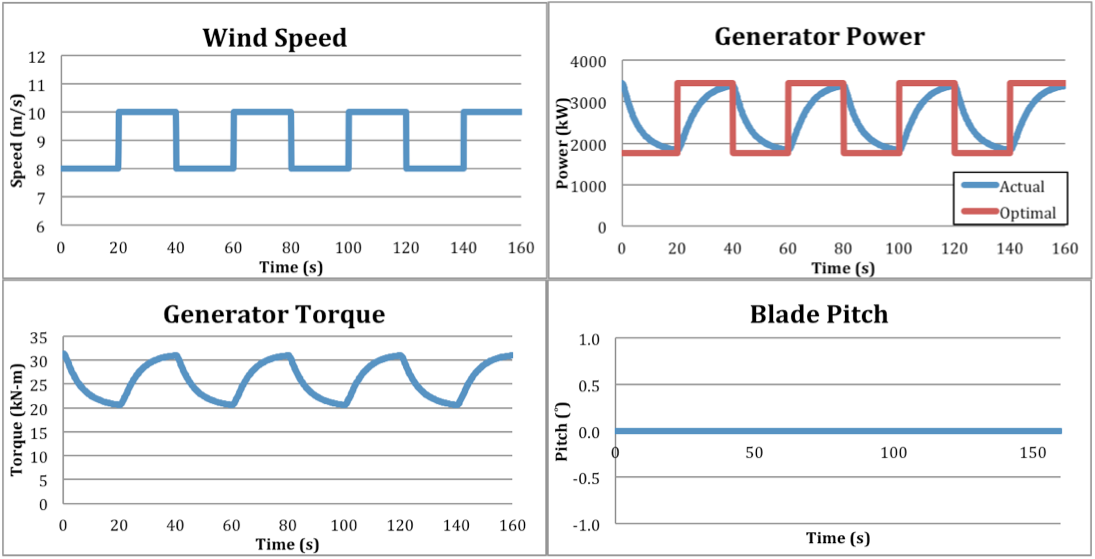
\includegraphics[width=\linewidth]{Figures/ch3Figures/fig3-3.png}
		
	\caption{NREL 5-MW response to wind speed fluctuations in control region 2.}
	\label{fig3-3}
\end{figure}

In Figure \ref{fig3-4} the turbine is subjected to a uniform incoming wind that changes between 16 m/s and 18 m/s every 40 seconds. These wind speeds are in region three, where optimal power production is the rated power of the turbine, 5 MW. After each change in wind speed the turbine experiences both spikes and dips in power production.  The largest fluctuations in power occur in the first 10 seconds after a change in wind speed. After 25 seconds the generated power is nearly constant at 5 MW.  In this case turbine performance is regulated by both torque control and pitch control. 

\begin{figure}[htbp]
	\centering
		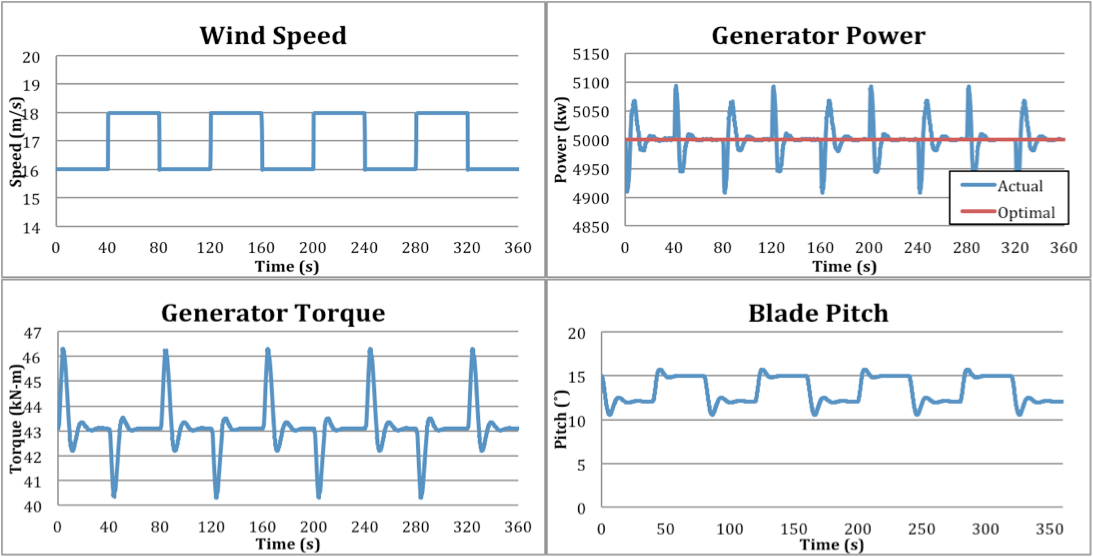
\includegraphics[width=\linewidth]{Figures/ch3Figures/fig3-4.png}
		
	\caption{NREL 5-MW response to wind speed fluctuations in control region 3.}
	\label{fig3-4}
\end{figure}

You can see from the previous figures that wind turbines respond reactively to changes in wind speed. However, several researchers have shown that turbine performance can be improved if a turbine is able to pre-emptively react to changes in wind speed before they occur. Ozdemir, Seiler, and Balas showed that perfect preview knowledge of incoming wind speed could be used to increase power production or decrease gearbox loads by improving generator torque control in region 2 operation. The authors used state space optimal control techniques to control generator torque based on incoming fluctuations in wind speed. In some of their simulations they were able to achieve increases in power generation of 6\% or decreases in gerabox loading of 30\%.\cite{ozdemir2013} Dunne, Pao, Wright, Jonkman, Kelley, and Simley have shown that perfect preview knowledge of incoming wind speed fluctuations could also be used reduce turbine loads by improving pitch control in region 3 operation. The authors examined three methods of feed forward pitch control based on wind speed preview information: non-causal series expansion, preview control, and optimized FIR filter methods. The autors simulated the response of the feed forward controllers to both turbulent wind and sudden gusts. Each of the feed forward controllers were capeable of reducing damage equivalent loads on the turbine blades and/or turbine tower. \cite{dunne2011}. Schlipf, along with various collaborators, has shown that imperfect preview knowledge of incoming wind speed, obtained through a nacelle mounted LIDAR, can be used to improve turbine control.\cite{schlipf2008,schlipf2010,schlipf2011,schlipf2011a,schlipf2013} Schlipf, Schlipf, and K{\"u}hn used simulations of the LIDAR and turbine to demonstrate that LIDAR based feed forward collective pitch control could reduce extreme and fatigue loads on turbine blades and the turbine tower. \cite{schlipf2013} However, Schlipf, Kapp, Anger, Bischoff, Hofs{\"a}{\ss}, Rettenmeier, and K{\"u}hn concluded that only minimal increases in power production could be achieved using LIDAR assisted generator torque control in region 2 operation.\cite{schlipf2011a}  Scholbrock, Fleming, Fingersh, Wright, Schlipf, Haizman, and Belen field tested a LIDAR assisted feed forward controller on the NREL CART3 research turbine. The authors observed reductions in damage equivalent loads for the turbine blade bending moments and rotor torque. \cite{scholbrock2013}

The remainder of chapter examines the feasibility of feed forward pitch control using wind speed preview information generated by using wind speed estimates from an upwind turbine. The following section describes how FAST, a single turbine simulation tool, can be used to simulate a two turbine system. Section 3 describes the feed forward controller. Sections 4 and 5 examine how the feed forward controller performs when subjected to wind gusts and turbulent wind. Section 6 examines how sensitive teh feed forward controller is to errors in feed forward wind speed estimate data and the corresponding implications.



%----------------------------------------------------------------------------------------
%	SECTION 2
%----------------------------------------------------------------------------------------

\section{Using FAST to Model a 2 Turbine System} \label{section3-2}

As discussed in Section \ref{section2-2}, FAST is a medium fidelity wind turbine simulation tool. FAST models both the aerodynamics and structural dynamics of a single turbine. FAST can model a turbine's response to either uniform incoming wind or, with the help of TurbSim, statistically accurate turblent wind. Though FAST only models one turbine at a time it can be used to model a multi turbine system if a few assumptions are made. Figure \ref{fig3-5} shows the two turbine system being simulated. The wind is blowing from left to right and the, the terain is flat, and the downwind turbine is slightly offset from the upwind turbine. When simulating this two turbine system in FAST the following assumptions are made:

\begin{itemize}
  \item Taylor's hypothesis is valid. The wind speed fluctuations experienced by the upwind turbine will propogate downwind at some convection velocity without changing. Therefore, the downwind turbine will experience the same series of wind speed fluctuations as the upwind turbine but at a later time.
  \item The slight offset of the downwind turbine will be enough to keep the downwind turbine out of the upwind turbine's wake.
  \item The slight offset of the downwind turbine will be small enough that wind speed fluctuations will hit both the upwind and downwind turbines.
  \item Because the terrain is flat, complex terrain effects do not need to be considered.
\end{itemize}


 \begin{figure}[htbp]
	\centering
		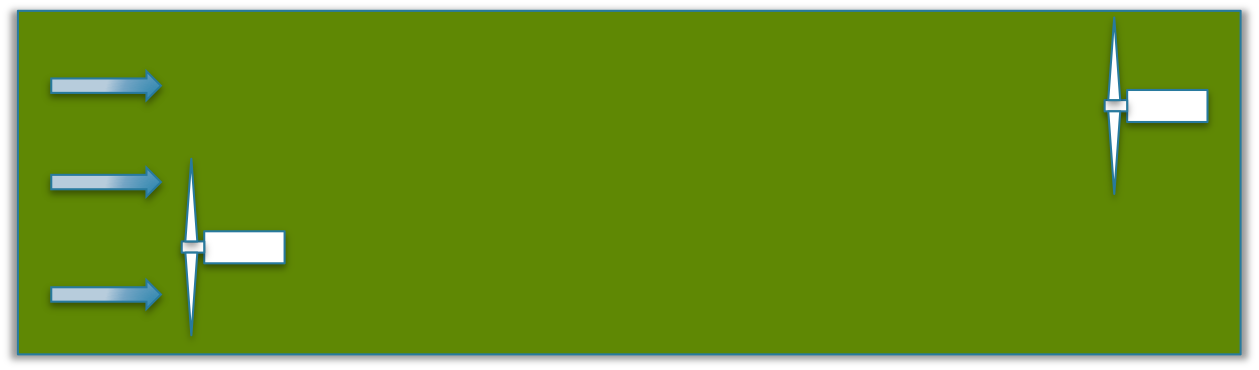
\includegraphics[width=\linewidth]{Figures/ch3Figures/fig3-5.png}
		
	\caption{Illustration of the two turbine system modeled in this chapter.}
	\label{fig3-5}
\end{figure}

Figure \ref{fig3-6} shows how FAST can be used to simulate the two turbine system illustrated in Figure \ref{fig3-5}. First a simulated wind field is generated. This can be a simple wind field, such as  uniform incoming wind, or a turbulent wind field generated with TurbSim. Next, FAST is used to simulate how a turbine with a conventional control system will respond to the  wind field. This first FAST simulation simulates the upwind turbine in our two turbine system. Once the first FAST simulation is complete the simulation results are post-processed using the wind speed estimation techniques described in \ref{section2-4}. In real world applicaions data from the upwind turbine would be continually processed and passed to the downwind turbine. However, since we are simulating the upwind and downwind turbine separately, it is easier to process all of the upwind turbine data at the same time. Finally, FAST is used to simulate the donwwind turbine. In this second simulation the turbine experiences the same wind field, but the turbine has feed forward pitch control and has access to wind speed preview data that was generated by post processing the results of the upwind turbine simulation. By comparing the simulation results from the first (upwind) and second (downwind) FAST simulations we can see how the feed forward pitch controller has affectetd turbine performance.

 \begin{figure}[htbp]
	\centering
		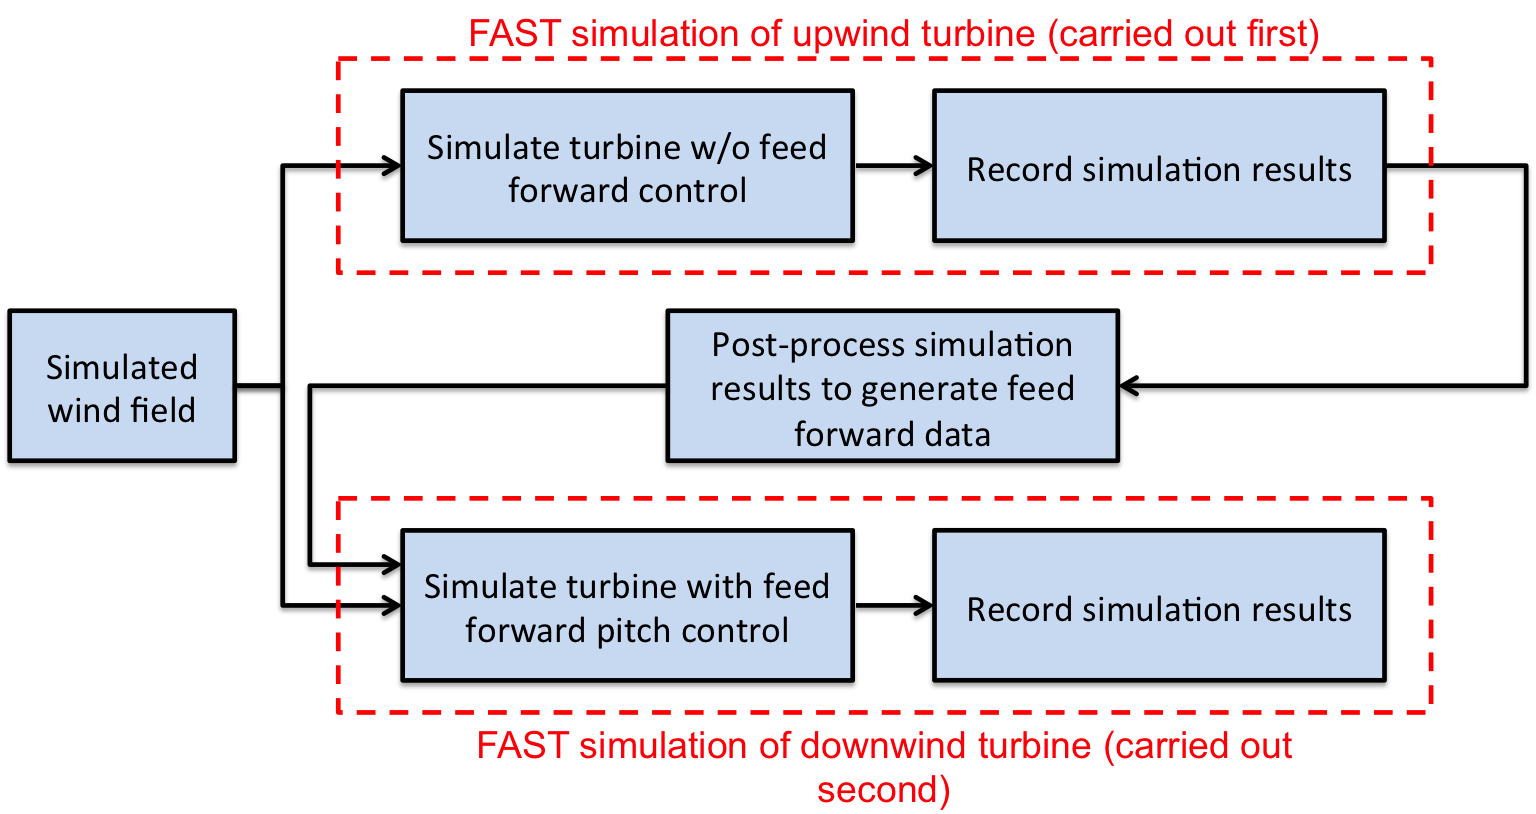
\includegraphics[width=\linewidth]{Figures/ch3Figures/fig3-6.png}
		
	\caption{How FAST can be used to simulate a two turbine system.}
	\label{fig3-6}
\end{figure}


%----------------------------------------------------------------------------------------
%	SECTION 3
%----------------------------------------------------------------------------------------

\section{Controller Design} \label{section3-3}

\subsection{Implementing Feed Forward Control} \label{section3-3-1}

Figure \ref{fig3-7} is a simple block diagram illustrating how the control system, turbine, and wind interact for a typical utility scale turbine. The behavior of the turbine is affected by the wind as well as the collective pitch ($\theta$) and generator torque ($T_{Gen}$) commands sent by the closed loop controller. The closed loop controller monitors the turbine rotor speed ($\Omega_{Rotor}$), the only feedback signal used in a typical utility scale turbine controller, to determine if the turbine is operating at a desired steady state operating point. If the turbine is not at a desired operating point the controller manipulates collective blade pitch ($\theta$) and generator torque ($T_{Gen}$) to bring the turbine to a desired operating point. In region 3 (high wind speeds) the controller tries to keep the turbine rotor speed ($\Omega_{Rotor}$) and power generation constant. In region 2 (low and medium wind speeds) the controller tries to maintain the rotor speed that will maximize power generation. From a control standpoint the wind is a disturbance, it is an uncontrolled input that affects the behavior of the turbine. Generally, changes in the wind cause the turbine to move away from desired operating points while the closed loop controller acts to bring the turbine back to desired operating points.


 \begin{figure}[htbp]
	\centering
		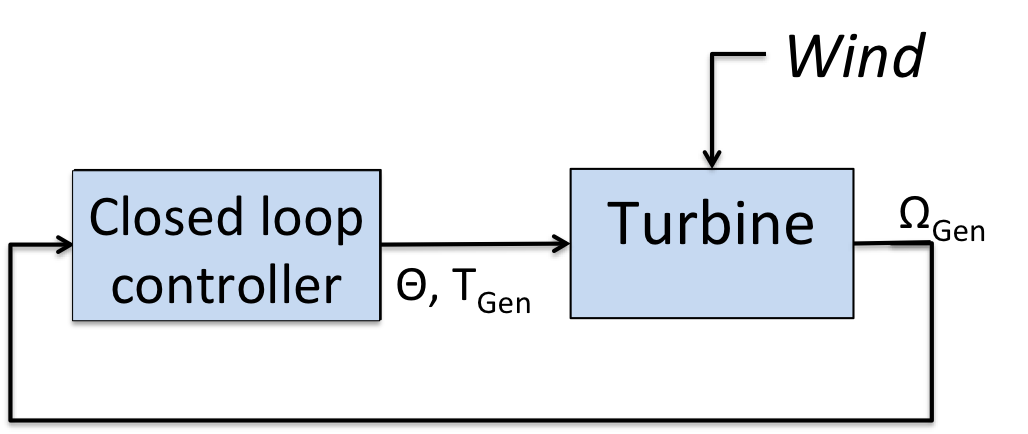
\includegraphics[width=.6\linewidth]{Figures/ch3Figures/fig3-7.png}
		
	\caption{Simple block diagram of turbine w/o feed forward control.}
	\label{fig3-7}
\end{figure}

Figure \ref{fig3-8} is a simple block diagram illustrating the method we have chosen  to incorporate feed forward control into the control system of a turbine. You can see that the feedback control loop shown in Figure \ref{fig3-7} remains intact, but a feed forward controller, which issues supplimental collective pitch ($\theta_{ff}$) and generator torque ($T_{ff}$) commands has been added. The closed loop controller shown in Figure \ref{fig3-8} is identical to the one in Figure \ref{fig3-7}. This is not the only way to implement feed forward control, but this method does have some advantages. It is fairly simple in that it does not require us to re-design the entire control system. In addition, if the turbine were to lose the feed forward signal for any reason it would simple begin operating as if it were using a standard closed loop turbine control system. In fact this feed forward control implementation allows the turbine to smoothly transition between standard closed loop control and closed loop with feed forward controll. This trait is desireable for a variety of situations. For example, if the wind changes direction the turbine may find that it no longer has an upwind turbine to use as a sensor.

 \begin{figure}[htbp]
	\centering
		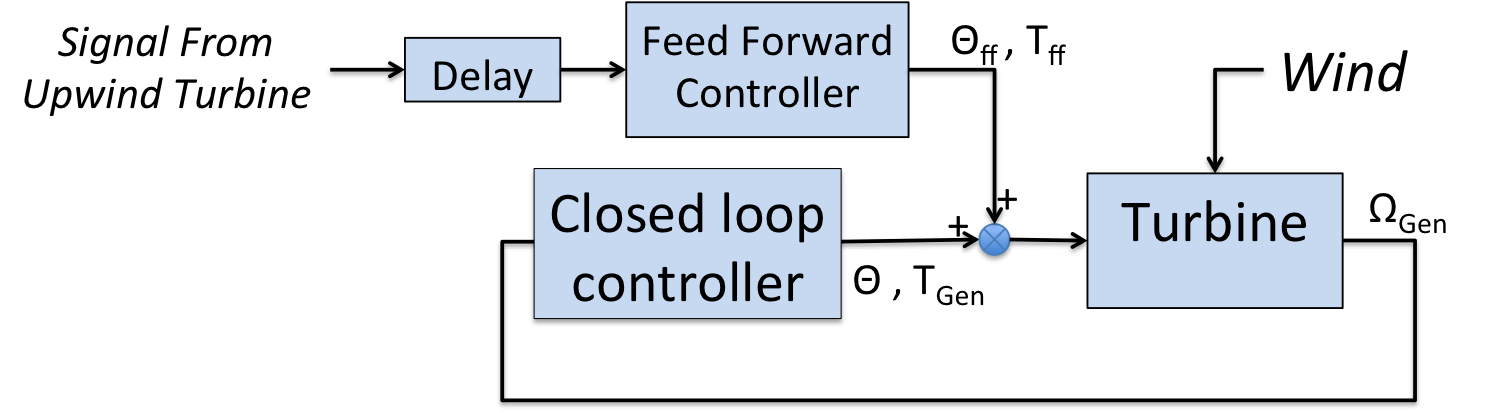
\includegraphics[width=\linewidth]{Figures/ch3Figures/fig3-8.png}
		
	\caption{Simple block diagram of turbine with feed forward control.}
	\label{fig3-8}
\end{figure}

\subsection{Closed Loop Controller}

The closed loop controller is modeled in Simulink and coupled to FAST as described in the FAST user's guide \cite{jonkman2005}, and the full Simulink model of the closed loop controller can be found in appendix \ref{AppendixB}. The controller has all the properties of the NREL 5-MW controller defined by NREL in \cite{jonkman2009} plus a model of the collective blade pitch actuator.  Figure \ref{fig3-9} illustrates the controller. The NREL 5-MW controller defined in \cite{jonkman2009} consists of a measurement filter, a torque controller, and a pitch controller. The measurement filter is a recursive, single pole low pass filter with a corner frequency of 0.25Hz. The purpose of this low pass filter is to mitigate high frequency excitations of the control system. The torque controller uses a torque schedule, basing generator torque on the rotational speed of the turbine. The pitch controller is a non-linear PI (proportional and integral) controller where the proportional and integral gains are a function of blade pitch. 

Since this chapter is concerned with feed forward pitch control, the turbine will be operating in control region 3 for all simulations. The NREL 5-MW turbine operates in control region 3 when wind speeds are higher that the turbine's rated wind speed of 11.4 m/s. in control region 3 the pitch controller varies collective blade pitch in an attempt to maintain a constant rotational rotor speed ($\omega_{Rotor}$) of 12.1 RPM. When the rotor is spinning at 12.1 RPM the generator supplies the rated generator torque (43,093.55 $N \cdot m$ ), but whe the 12.1 RPM the torque controller varies torque in an effort to maintain a constant power generation of 5 MW. 

The controller shown in figure \ref{fig3-9} also includes a model of the collective pitch actuator. Though the pitch actuator is not part of the control system it must be modeled in Simulink because current versions of FAST do not model pitch actuator dynamics. If pitch actuator dynamics are not modeled the closed loop controller is able to instantly change blade pitch. This is physically unrealistic and in some circumstances it leads to unrealistic control system behavior, such as high frequency fluctuations in pitch or unrealistic reactions to feed forward pitch control.

 \begin{figure}[htbp]
	\centering
		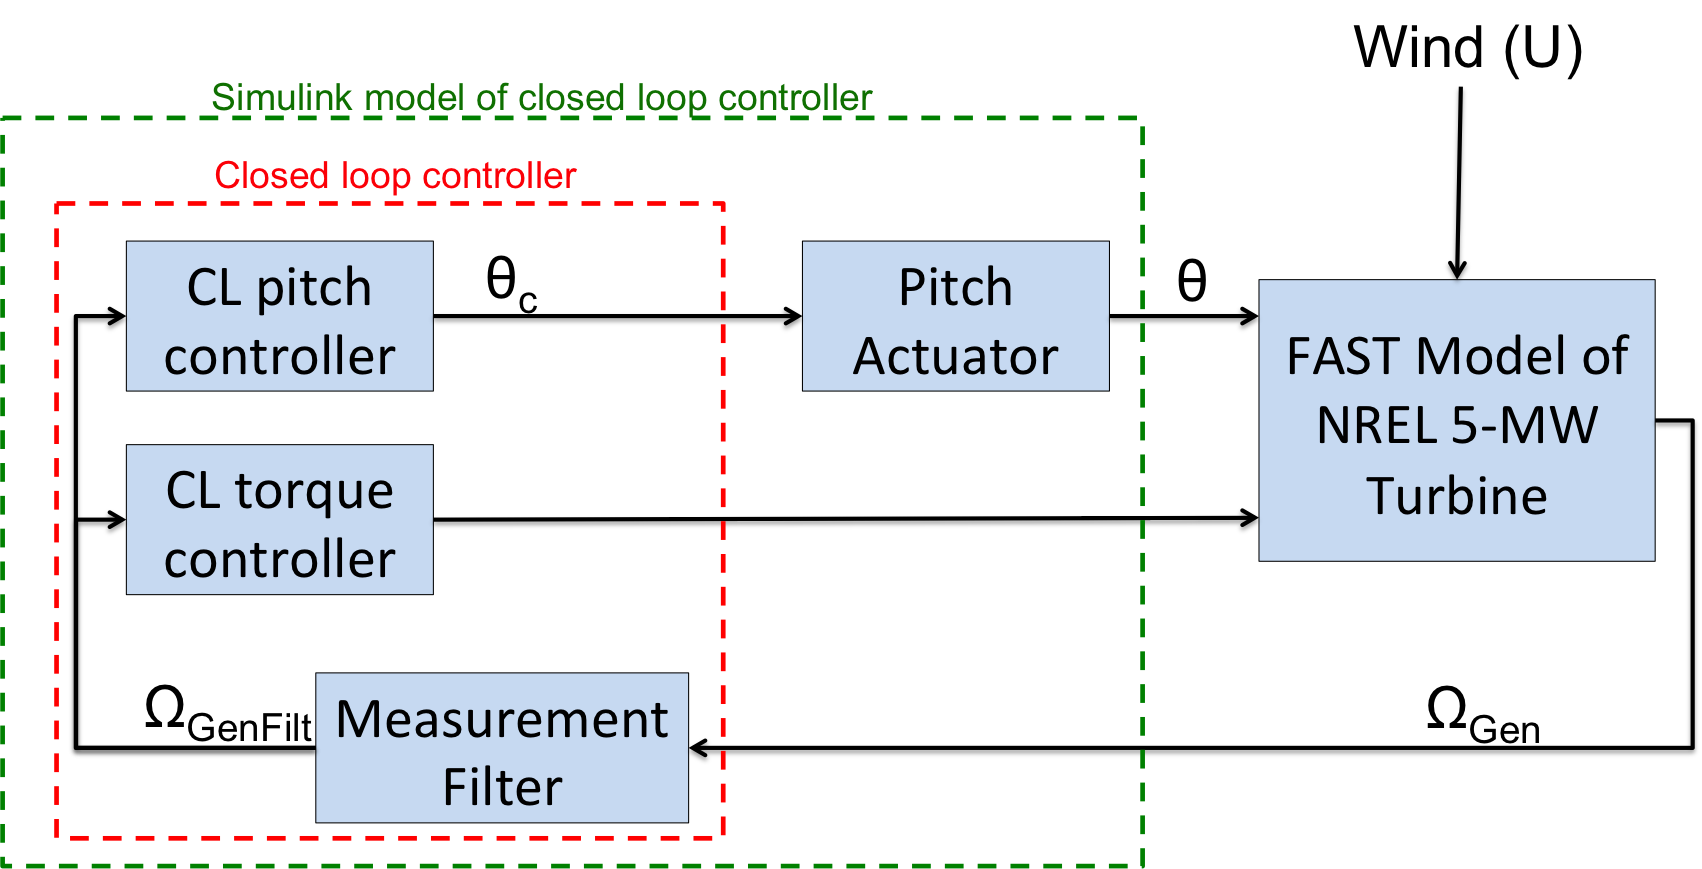
\includegraphics[width=\linewidth]{Figures/ch3Figures/fig3-9.png}
		
	\caption{Closed loop control system.}
	\label{fig3-9}
\end{figure}

The pitch actuator is modeled as a second order system with dynamics describe by equation \ref{eq3-1}, where  $\theta$  is the actual collective blade pitch, $\theta_c$ is the desired blade pitch requested by the controller, $\xi$ is the damping ratio of the pitch actuator, and $\omega_o$ is the undamped natural frequency of the pitch actuator. Jonkman does define a NREL 5-MW blade pitch actuator in \cite{jonkman2009}, but Jonkman has admitted that the pitch actuator defined in \cite{jonkman2009} is very fast and is unrealistic \cite{jonkman2014}. Instead we use $\xi = 0.7$ and $\omega_o = 1Hz$, which have been used to model NREL 5-MW pitcha actuators in previous research on feed forward turbine pitch control\cite{dunne2011,dunne2012}. 

\begin{equation}
	\ddot{\theta } + 2\xi \omega_o \dot{\theta} + \omega_{o}^{2}\theta = \omega_{o}^{2}\theta_c \label{eq3-1}
\end{equation}




\subsection{Feed Forward Controller} \label{section3-3-3}

The feed forward controller is based on the dynamic feed forward pitch controller proposed by Shlipf in \cite{schlipf2010}. Figure \ref{fig3-10} illustrates how the feed forward controller interfaces with the closed loop controller described in the previous section. As described in Section \ref{section3-3-1}, the wind is a disturbance, an uncontrolled input that affects sytem behavior. Typically, changes in the wind cause the turbine to deviate from the desired operating conditions while the closed loop controller acts to bring the turbine back to the desired operating conditions. Ideally we would like the feed forward controller to cancel out the effect of the disturbance so the turbine never deviates from the desired operating conditions to begin with and the closed loop controler would not need to act.

 \begin{figure}[htbp]
	\centering
		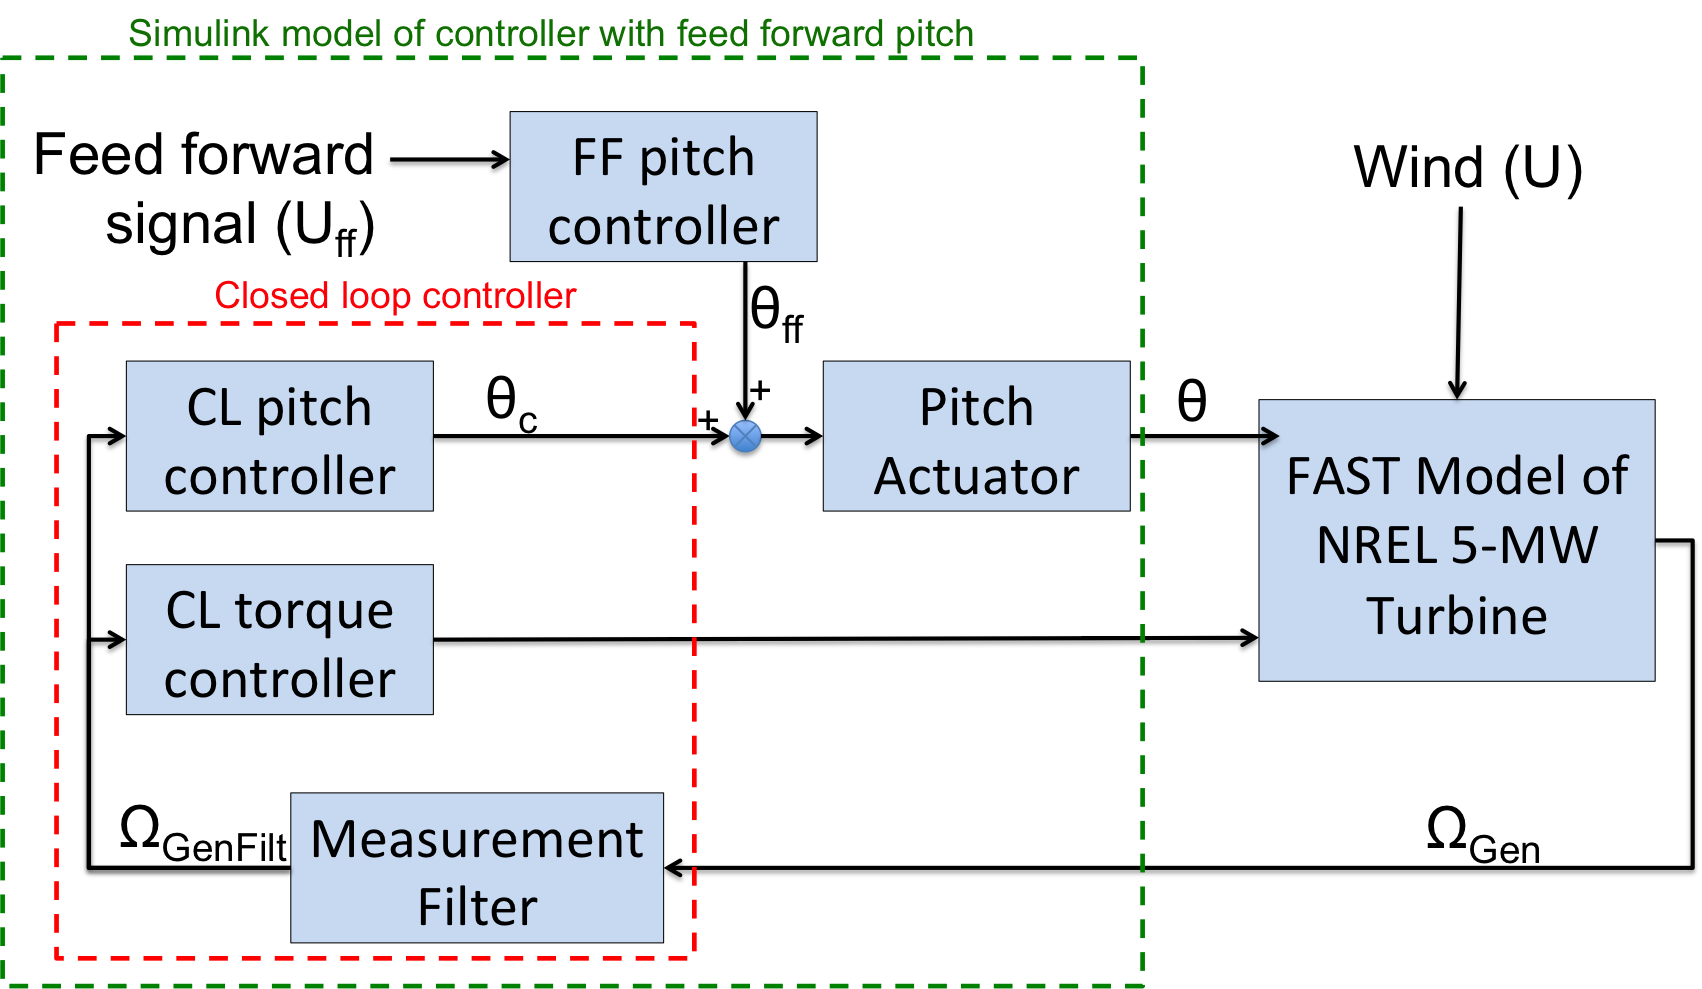
\includegraphics[width=\linewidth]{Figures/ch3Figures/fig3-10.png}
		
	\caption{Controller with feed forward and closed loop control.}
	\label{fig3-10}
\end{figure}

As discussed in the previous section, the goal of region 3 pitch control is to maintain a constant rotor speed of 12.1 RPM. This constant rotor speed is maintained when the aerodynamic torque applied to the rotor by the wind is equal to the torque applied to the rotor by the generator and there is no net torque to accellerate or decellerate the rotor. If the rotor is spinning at 12.1 RPM and the wind speed is anywhere between the rated wind speed (11.4 m/s) and the cutout wind speed (25 m/s) of the turbine there is a pitch angle ($\theta$) that will cause an aerodynamic torque on the rotor that perfectly matches the torque applied to the rotor by the generator. We'll call this pitch angle the steady state pitch ($\theta_{ss}$). Though the steady state pitch can't be calculated it can estimated through simulation. The relationship between steady state pitch and wind speed is shown in Figure \ref{fig3-11}.

 \begin{figure}[htbp]
	\centering
		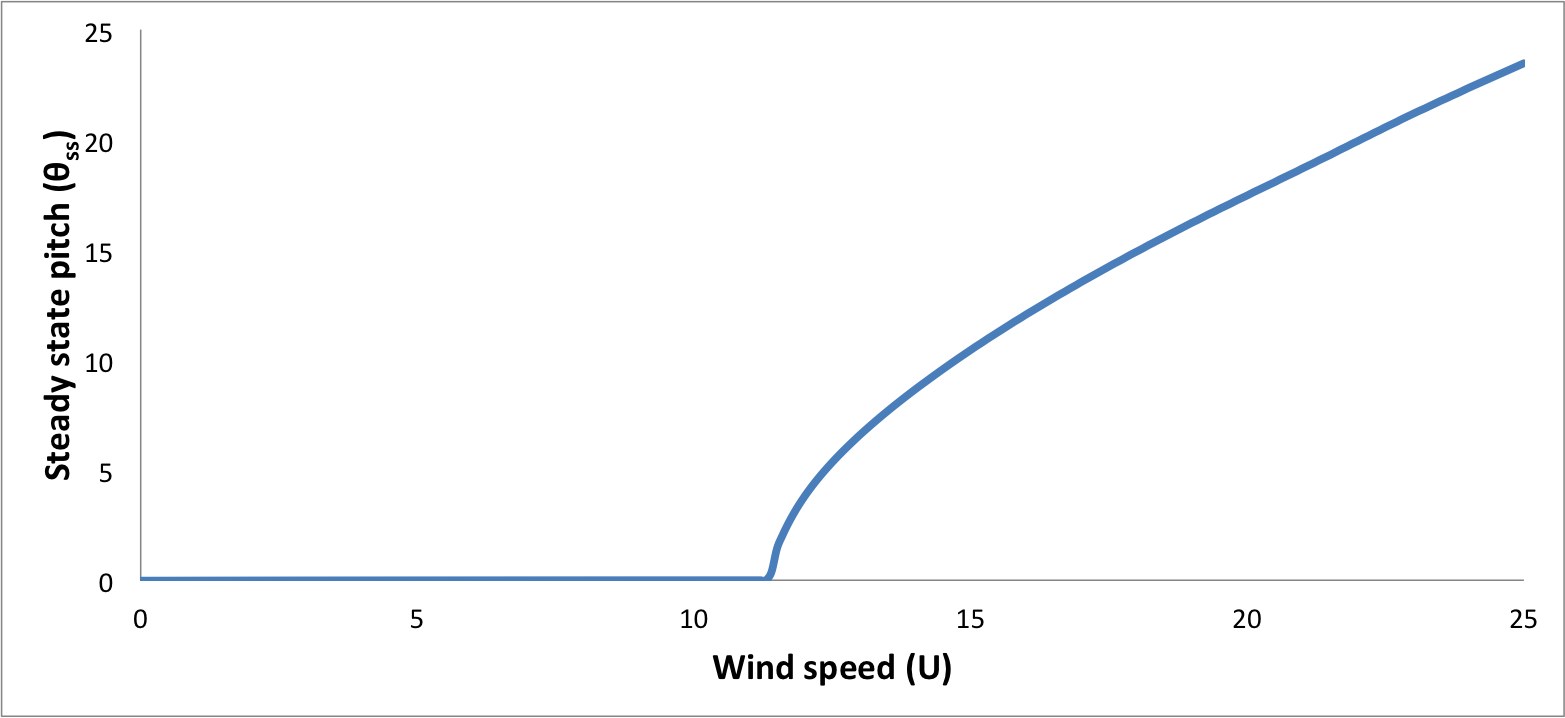
\includegraphics[width=\linewidth]{Figures/ch3Figures/fig3-11.png}
		
	\caption{Steady state pitch ($\theta_{s}$) as a function of incoming wind speed.}
	\label{fig3-11}
\end{figure}

If the collective blade pitch of the turbine ($\theta$) allways matches the steady state pitch ($\theta_{ss}$) for the incoming wind speed ($U$) then the turbine will never deviate from the rated rotor speed of 12.1 RPM. If the feed forward signal $U_{ff}$ is an accurate estimate of the incoming wind speed (U) then it is possible to design a feed forward controller that causes the collective blade pitch to allways match the corresponding steady state pitch. Since all pitch commands pass through the pitch actuators we can only ensure the correct feed forward pitch signal if we first pass the feed forward signal $U_{ff}$ through a function that inverts the dynamics of the blade pitch actuator. Therefore, the pitch commands supplied by the feed forward pitch controller ($\theta_{ff}$) is given by the equations \ref{eq3-2} and \ref{eq3-3}. $\theta_{ss}$ is the steady state pitch function that was experimentally determined and is illustrated in Figure \ref{fig3-11}. $U_{ffd}$ is the dynamic feed forward velocity, which accounts for and cancels out the dynamics of the pitch actuator.

\begin{equation}
	\theta_{ff} =  \theta_{ss}(U_{ffd}) \label{eq3-2}
\end{equation}

\begin{equation}
	U_{ffd} =  (\ddot{U} + 2 \xi \omega_o \dot{U} + \omega_o^2 U) / \omega_o^2 \label{eq3-3}
\end{equation}

If the feed forward wind speed estimate $U_{ff}$ is perfectly accurate then the feed forward signal generated using equations \ref{eq3-2} and \ref{eq3-2} will completely compensate for fluctuations in wind speed and the closed loop controller will never issue a pitch command. However, we know that in practice $U_{ff}$ will not be a perfect estimate of incoming wind speed and the closed loop controller will act whenever the feed forward pitch controller does not perfectly compensate for fluctuations in wind speed.

%----------------------------------------------------------------------------------------
%	SECTION 4
%----------------------------------------------------------------------------------------
\section{Performance With Perfect Wind Speed \\
		Knowledge} \label{section3-4}

Now that the feed forward control system has been defined the performance of this feed forward control system can be examined. In the following sections we examine the performance of the feed forward controller when it has perfect knowledge of the incoming wind speed. Two wind cases are examined. The first case is a large gust. These occur infrequently, but can be very damaging to a turbine. The second case is a turbulent wind inflow, which is typical of what a turbine experiences in day to day operation. in In any real world implementation of this control system the feed forward controller will have imperfect knowledge of the incoming wind. As discussed in Chapter \ref{Chapter2}, a wind speed estimator provides imperfect estimates of both the wind speed (see Section  \ref{section2-4-1}) and convection velocity (see Section \ref{section2-5}). In addition, we know that Taylor's frozen turbulence hypothesis is not entirely accurate in practice and the wind speed fluctuations experienced by the downwind turbine will not be identical to the wind speed fluctuations experienced by the upwind turbine. However, simulating the feed forward control system with perfect knowledge of the incoming wind speed can provide valuable insight into the behavior of the feed forward control system, and can demonstrate the performance improvements that might be possible when the feed forward controller described in Section \ref{section3-3} is operated in ideal conditions. 



%----------------------------------------------------------------------------------------
%	SUBSECTION 4-1
%----------------------------------------------------------------------------------------
\subsection{Gust Response}\label{section3-4-1}

Figure \ref{fig3-12} shows an extreme operating gust for an NREL 5-MW turbine operating in 16 m/s wind according to IEC 61400-1 \cite{IEC2005}. Though extreme operating gusts occur infrequently, they can be very damaging to a wind turbine when they do occur. To examine the system's response to this extreme operating gust, both the upwind turbine and downwind turbine are subjected to a uniform wind inflow (i.e. the wind has no turbulence and all points on the turbine rotor are subjected to the same wind speed) with the magnitude shown in Figure \ref{fig3-12}. Since we are assuming the feed forward controller has perfect knowledge of the incoming wind speed, the wind speed information in Figure \ref{fig3-12} is also used as the feed forward wind speed estimate.


\begin{figure}[htbp]
	\centering
		\includegraphics[trim = {1cm 0 2cm 0}, clip, width = \linewidth]{Figures/ch3Figures/fig3-12.png}
		
	\caption{Extreme operating gust.}
	\label{fig3-12}
\end{figure}


Figures \ref{fig3-13} through \ref{fig3-17} illustrate how the upwind and downwind turbines respond to the 16 m/s extreme operating gust, while Table \ref{Table3-1} is a summary of some of the performance metrics that will be discussed in the following paragraph. By comparing the response of the upwind turbine, which does not have feed forward pitch control, to the response of the downwind turbine, which does have feed forward pith control, we can see how feed forward pitch control affects turbine performance.

In Figure \ref{fig3-13} we see that the turbine with feed forward pitch control (the downwind turbine) responds to the gust sooner than the turbine without feed forward control (the upwind turbine). This is unsurprising. As discussed in Section \ref{section3-1}, a turbine using only closed loop control will respond reactively to changes in turbine behavior, which are caused by changes in wind speed. On the other hand, a turbine with feed forward control can respond to changes in wind speed before they affect turbine behavior. In fact, a perfect feed forward controller would prevent the wind speed changes from affecting turbine behavior at all. We can also see in Figure \ref{fig3-13} that the turbine with feed forward control has  higher maximum pitch angle when responding to the gust, and that the blade motion has less transient behavior after the gust passes.

\begin{figure}[htbp]
	\centering
		\includegraphics[trim = {1cm 0 2cm 0}, clip, width = \linewidth]{Figures/ch3Figures/fig3-13.png}
		
	\caption{Blade pitch response to extreme operating gust. }
	\label{fig3-13}
\end{figure}

Figure \ref{fig3-14} shows that deviations from the rated rotor speed of 12 RPM are greatly reduced with feed forward control. The turbine with feed forward control has a maximum rotor speed of 12.07 RPM, which is only 0.6$\%$ over the rated speed. Without feed forward control, the rotor speed reaches a peak value of 14.15 RPM, which is 17.9$\%$ over the rated rotor speed. A 17.9$\%$ rotor over speed can be problematic as it may cause an emergency shut down of the turbine. According to Tobias Wehrhan of Oak Engineering LLC the threshold for an over speed shut down is usually 15-20$\%$ over the rated rotor speed, depending on the turbine (personal communication,March 19, 2015). Once an over speed shut down has been initiated, the turbine stops generating power until it can be safely restarted. This can lead to a significant loss of generated energy and therefore a loss of revenue for the turbine operator.

\begin{figure}[htbp]
	\centering
		\includegraphics[trim = {1cm 0 2cm 0}, clip, width = \linewidth]{Figures/ch3Figures/fig3-14.png}
		
	\caption{Rotor speed for turbine subjected to extreme operating gust. }
	\label{fig3-14}
\end{figure}

Figure \ref{fig3-15} shows that deviations from the rated power are greatly reduced with feed forward control. It is desirable to limit spikes in power. Power spikes can cause an emergency shut down of the turbine if it drives the DC-bus voltage above safe levels, which is typically 15-18$\%$ above the nominal DC-bus voltage (Tobias Wehrhan, personal communication,March 19, 2015). FAST does not model the DC-bus voltage, so these results don't show how close the turbine without feed forward control comes to triggering an over voltage shut-down. Table \ref{Table3-1} shows the total energy generated in each simulation. We see that the performance improvemments from feed forward control are achieved without a cost to energy generation. The turbine with feed forward control actually generates slightly more power than the turbine without feed forward control.


\begin{figure}[htbp]
	\centering
		\includegraphics[trim = {1cm 0 2cm 0}, clip, width = \linewidth]{Figures/ch3Figures/fig3-15.png}
		
	\caption{Power generation for turbine subjected to extreme operating gust.}
	\label{fig3-15}
\end{figure}

Excessive structural loading can cause turbine components to immediately fail, or can cause excessive wear and tear that shortens the life of turbine components. When turbine components fail the turbine must be shut down and repaired. If we can reduce the frequency of shut downs and repairs we can increase the revenue (by increasing energy generation) and decrease the cost to the turbine operator. There are many turbine components that can experience damage from gust loading. In this section we have chosen to examine two loads, the fore-aft bending moment at the base of the tower (Figure \ref{fig3-16}) and bending moment at the root of one of the turbine blades (Figure \ref{fig3-17}).We see similar behavior in both Figures. The turbine with feed forward control experiences lower loads during the extreme operating gust, while experiencing nearly identical loads at all other times. The feed forward controller reduces the maximum tower bending moment from 100,030 kNm to 50,900 kNm, a reduction of nearly 50$\%$, and reduces the aximum blade root moment from 11,617 kNm to 7,351 kNm, a reduction of 37$\%$.

\begin{figure}[htbp]
	\centering
		\includegraphics[trim = {1cm 0 2cm 0}, clip, width = \linewidth]{Figures/ch3Figures/fig3-16.png}
		
	\caption{Tower base fore-aft moment for turbine subjected to extreme operating gust.}
	\label{fig3-16}
\end{figure}

\begin{figure}[htbp]
	\centering
		\includegraphics[trim = {1cm 0 2cm 0}, clip, width = \linewidth]{Figures/ch3Figures/fig3-17.png}
		
	\caption{Blade root bending moment for turbine subjected to extreme operating gust.}
	\label{fig3-17}
\end{figure}

Table \ref{Table3-1} summarizes the performance metrics that have been discussed in this subsection. We see that feed forward control has significantly reduced structural loading of the turbine without decreasing energy generation. This can potentially lead to a reduction in the repair and maintenance costs of the turbine without a reduction in revenue from the turbine. The turbine without feed forward control experienced a 17.9$\%$ rotor over speed, which may be enough to induce an emergency shutdown of the turbine. Over speed shut down faults are not modeled in theses simulations, but if the turbine without feed forward control experienced an over speed shut down then it would generate significantly less energy than the turbine with feed forward control. In that scenario the turbine with feed forward control would have lower repair and maintenance costs while having higher revenue from energy generation.

\begin{table}
\centering
\begin{tabular}{ c | c c c c }
\hline
\hline
Turbine			& Max tower	base		& Max blade	root		& Max rotor				& Energy\\
Control			& bending moment		& bending moment		& over speed					& generated\\
					& (MNm)  				& (MNm)				& ($\%$)	& (kW hr)\\
\hline
  &  &   &  &  \\
Closed loop  & 100.00 & 11.62  &17.9 & 831.74 \\
 &  &   &  & \\
Closed loop  &  &   &  &  \\
with feed  & 50.90 & 7.35  & 0.6 & 831.75 \\
forward  &  &   &  &  \\
\hline
\hline
\end{tabular}
\caption{Extreme operating gust response with perfect wind speed knowledge.}
\label{Table3-1}
\end{table}

%----------------------------------------------------------------------------------------
%	SUBSECTION 4-2
%----------------------------------------------------------------------------------------
\subsection{Turbulent Wind Response} \label{section3-4-2}

In this subsection we examine how our two turbine system reacts to turbulent wind. Like the previous subsection both the upwind turbine and downwind turbine are subjected to the same wind speed fluctuations. The downwind turbine is equipped with the feed forward controller described in Subsection \ref{section3-3-3} and is assumed to have perfect knowledge of the incoming wind. The feed forward controller relies on knowledge of the incoming wind speed and the derivatives of the incoming wind speed. However, in a turbulent wind field the wind speed is not constant over the swept area of the rotor so there is no single measurement that can be considered the true incoming wind speed. In this subsection we will treat the average wind speed over the swept area of the rotor as the wind speed. Because this rotor average wind speed has some high frequency fluctuations it is passed through a single pole low-pass filter with a corner frequency of 0.5 Hz to generate the feed forward wind speed.

Figure \ref{fig3-18} shows the rotor average wind speed and feed forward wind speed for 200 seconds of the turbulent wind field used in this subsection. The complete wind field is 600 seconds long and was generated by TurbSim using a 16 m/s mean wind speed and the GPLLJ turbulence model. This was one of the 66 test cases used in Chapter \ref{Chapter2} and more details about this test case can be found in Section \ref{section2-2}. Figures \ref{fig3-19} through \ref{fig3-20} illustrate how the upwind and downwind turbines respond to the turbulent wind field. All figures in this subsection have the same axes as the corresponding figures in Subsection \ref{section3-4-1}. This helps illustrate the differences in magnitude between the wind turbine response to an extreme operating gust and the wind turbine response to a turbulent wind field with the same mean wind speed.

\begin{figure}[htbp]
	\centering
		\includegraphics[trim = {1cm 0 2cm 0}, clip, width = \linewidth]{Figures/ch3Figures/fig3-18.png}
		
	\caption{Rotor average wind speed and feed forward wind speed for 16m/s turbulent wind.}
	\label{fig3-18}
\end{figure}

In Figure \ref{fig3-19} we see the blade pitch response of each turbine. We see that the blade pitch response of each turbine follows a similar pattern of peaks and valleys. However, for the turbine with feed forward pitch control the peaks and valleys occurs a few seconds earlier. This is expected because both turbines are reacting to the same fluctuations in wind speed but the turbine with feed forward control can react to those wind speed fluctuations before they affect turbine behavior. 

\begin{figure}[htbp]
	\centering
		\includegraphics[trim = {1cm 0 2cm 0}, clip, width = \linewidth]{Figures/ch3Figures/fig3-19.png}
		
	\caption{Blade pitch response to 16m/s turbulent wind.}
	\label{fig3-19}
\end{figure}

Figures \ref{fig3-20} and \ref{fig3-21} show that the feed forward controller  reduces deviations in both rotor speed and power. With feed forward control the rotor speed stays within ???$\%$ of the rated rotor speed and the power stays within ???$\%$ of the rated power. Without feed forward control the rotor speed deviates as much as ???$\%$ from the rated speed and the power deviates as much as ???$\%$ from the rated power. Though the turbine with feed forward control performs better than the turbine without feed forward control it is important to note that neither turbine has a spike in rotor speed or power that could trigger an emergency shut down.

\begin{figure}[htbp]
	\centering
		\includegraphics[trim = {1cm 0 2cm 0}, clip, width = \linewidth]{Figures/ch3Figures/fig3-20.png}
		
	\caption{Rotor speed for turbine in 16m/s turbulent wind.}
	\label{fig3-20}
\end{figure}

\begin{figure}[htbp]
	\centering
		\includegraphics[trim = {1cm 0 2cm 0}, clip, width = \linewidth]{Figures/ch3Figures/fig3-21.png}
		
	\caption{Power generation for turbine in 16m/s turbulent wind.}
	\label{fig3-21}
\end{figure}

Figures \ref{fig3-22} and \ref{fig3-23} show the tower fore-aft bending moment and the blade root bending moment. In the previous subsection, when we examined the turbines' responses to an extreme operating gust, it was immediately obvious that feed forward control significantly reduced loads. In figures \ref{fig3-22} and \ref{fig3-23} it is not obvious that feed forward control is reducing loads. Though there are many moments in the simulation when feed forward control reduces loading, there are also many times when feed forward control causes higher loading. To determine which control system has better performance we must statistically analyze the loading.

In the previous subsection we analyzed loading by measuring and comparing the maximum loads experienced by the turbines. For these simulation results comparing the maximum loads doesn't make sense. In the previous subsection the turbine experienced a single large spike in loading when the extreme operating gust hit the turbines. In this subsection the turbine experiences many loading cycles that all have similar amplitudes. 


\begin{figure}[htbp]
	\centering
		\includegraphics[trim = {1cm 0 2cm 0}, clip, width = \linewidth]{Figures/ch3Figures/fig3-22.png}
		
	\caption{Tower base fore-aft moment for turbine in 16m/s turbulent wind.}
	\label{fig3-22}
\end{figure}

\begin{figure}[htbp]
	\centering
		\includegraphics[trim = {1cm 0 2cm 0}, clip, width = \linewidth]{Figures/ch3Figures/fig3-23.png}
		
	\caption{Blade root bending moment for turbine in 16m/s turbulent wind.}
	\label{fig3-23}
\end{figure}

Table \ref{Table3-2} shows the mean and standard deviation of several turbine performance metrics. We see that feed forward control does not affect the mean values, but does decrease the variability of the performance metrics. Feed forward control reduces the standard deviation of the Power by more than 50$\%$. 

Reduced variability in power generation can be beneficial for grid integration of wind turbines. The standard deviation of the tower base bending moment and the blade root bending moment are reduces by 26$\%$ and 2$\%$ respectively. 

\begin{table}
\centering
\begin{tabular}{ c | c c c c c c c c c c c c}
\hline
\hline
	& & \multicolumn{2}{c}{Tower base}	& & \multicolumn{2}{c}{Blade root}		& & \\
	& & \multicolumn{2}{c}{bending}	& & \multicolumn{2}{c}{bending}		& &\multicolumn{2}{c}{Rotor}	& & \\
	& & \multicolumn{2}{c}{moment}	& & \multicolumn{2}{c}{moment}		& &\multicolumn{2}{c}{speed}		& &\multicolumn{2}{c}{Power} \\	
Turbine					& & \multicolumn{2}{c}{(MNm)}  					& & \multicolumn{2}{c}{(MNm)}	& & \multicolumn{2}{c}{(RPM)}	& & \multicolumn{2}{c}{(kW)}\\
\cline{3-4} \cline{6-7} \cline{9-10} \cline{12-13} 
Control & & mean & $\sigma$ & & mean & $\sigma$ & & mean & $\sigma$  & & mean & $\sigma$ \\
\hline
\\
Closed loop & & 36.60 & 4.64  & & 5.96 & 1.84  && 12.0 & 0.212&& 5,000  & 21.8 \\
 \\
Closed loop \\
with feed   & & 36.60 & 3.42  & & 5.95 & 1.80 && 12.0 & 0.0547  && 5,000  & 10.7 \\
forward\\
\hline
\hline
\end{tabular}
\caption{Statistical summary of turbine performance in 16m/s wind.}
\label{Table3-2}
\end{table}


Though a reduction in the standard deviation of the structural loads is noteworthy, it is more important to understand how the changes in structural loads will affect the wear and tear on turbine components. To estimate the wear and tear inflicted on the tower base and the blade root we can calculate the short term damage equivalent loads (DEL). An explanation of damage equivalent loads and how they were calculated in this dissertation can be found in Appendix \ref{AppendixC}. 

Table shows that for this 10 minute simulation of 16m/s turbulent wind feed forward control reduces the damage equivalent loads for both tower base bending moment and blade root bending moment. This indicates that the turbine with feed forward control experiences less wear and tear on it's components, which may lead to less repair and maintenance costs over the life of the turbine.


\begin{table}
\centering
\begin{tabular}{ c | c c c c c c c c c}
\hline
\hline
					&&\multicolumn{2}{c}{Tower base}					&&\multicolumn{2}{c}{Blade	root} \\
					&&\multicolumn{2}{c}{bending moment}			&&\multicolumn{2}{c}{bending moment}\\
						\cline{3-4} 														\cline{6-7}
Turbine			&& DEL   	& Change										&& DEL  	& Change\\
Control			&& (MNm)  & in DEL 										&& (MNm)  & in DEL 	\\
\hline
\\
Closed loop  && 44.20 & - 													&& 10.58 & - \\
 \\
Closed loop\\
with feed  		&& 35.60 & -19.5$\%$ 									&& 10.02 & -5.3$\%$\\
forward\\
\hline
\hline
\end{tabular}
\caption{Short term damage equivalent loads for 570s simulation of turbine  in 16m/s turbulent wind.}
\label{Table3-3}
\end{table}


%----------------------------------------------------------------------------------------
%	SECTION 5
%----------------------------------------------------------------------------------------
\section{Performance With Wind Speed Estimate From Upwind Turbine} \label{section3-5}
The previous sections demonstrated how the feed forward pitch controller affects performance when it has perfect knowledge of the incoming wind. However, in practice the feed forward controller will not have perfect knowledge of the incoming wind. The feed forward controller will have an estimate of the incoming wind that is generated by using the upwind turbine as a sensor. In the following subsections we examine the performance of the feed forward controller when it has only an estimate of the incoming wind speed. The incoming wind speed estimate is based on the dynamic behavior of the upwind turbine and is generated using the process described in Section \ref{section2-4}. The simulations described below assume Taylor's frozen turbulence, and assume that we will be able to perfectly determine the convection velocity. We know that neither of those assumptions will be entirely accurate in practice, but the simulations described in this section bring us a step closer to a realistic implementation of feed forward pitch control than the simulations described in the previous section.

%----------------------------------------------------------------------------------------
%	SUBSECTION 5-1
%----------------------------------------------------------------------------------------
\subsection{Gust Response} \label{section3-5-1}
Figure \ref{fig3-24} shows an extreme operating gust for an NREL 5-MW turbine operating in 16 m/s wind according to IEC 61400-1 \cite{IEC2005} and the feed forward wind speed estimate generated by the upwind turbine. This is the same extreme operating gust simulated in Section \ref{section3-4-1}. The feed forward wind speed estimate does not perfectly capture the fluctuations in wind speed. In particular, the feed forward wind speed estimate has smaller peaks and valleys and contains some transient behavior after the extreme operating gust has passed.



\begin{figure}[htbp]
	\centering
		\includegraphics[trim = {1cm 0 2cm 0}, clip, width = \linewidth]{Figures/ch3Figures/fig3-24.png}
		
	\caption{Extreme operating gust and feed forward wind speed estimate based on gust.}
	\label{fig3-24}
\end{figure}

Figure \ref{fig3-25} shows the pitch response of the turbines. As we saw in previous simulations, the turbine with feed forward pitch control reacts to the extreme operating gust sooner than the turbine without feed forward pitch control. One noteworthy feature is the large dip in blade pitch for the turbine with feed forward pitch control. The blade pitch briefly drops to 5.4$^\circ$ at approximately 110 seconds. This is potentially dangerous behavior for the turbine with feed forward pitch control. For a given wind speed, decreasing the blade pitch results in an increase in the wind energy captured by the rotor. This leads to increased structural loads and increased rotor speed. If the blade pitch suddenly drops too low, as may be the case here, it can potentially lead to spikes in structural loads or rotor speed. 

\begin{figure}[htbp]
	\centering
		\includegraphics[trim = {1cm 0 2cm 0}, clip, width = \linewidth]{Figures/ch3Figures/fig3-25.png}
		
	\caption{Blade pitch response to extreme operating gust. }
	\label{fig3-25}
\end{figure}

Figure \ref{fig3-26} shows that feed forward control significantly reduces deviations from the rated rotor speed of 12 RPM. The turbine without feed forward pitch control has a maximum rotor speed 17.9$\%$ above the rated speed. As discussed before, an overspeed of this magnitude could cause an emergency shutdown of the turbine. The turbine with feed forward pitch control has a maximum rotor speed 5.5$\%$ above the rated speed. For the turbine without feed forward control the maximum rotor speed occurs immediately after the peak of the extreme operating gust. The turbine with feed forward pitch control also has a rotor overspeed immediately after the peak of the extreme operating gust, but the maximum rotor speed occurs approximately 10 seconds later, immediately after the sudden dip in blade pitch that was observed in Figure \ref{fig3-25}. This suggests that the larges rotor overspeed experienced turbine with feed forward pitch control was caused by the control action of the feed forward controller and not by the extreme operating gust.

\begin{figure}[htbp]
	\centering
		\includegraphics[trim = {1cm 0 2cm 0}, clip, width = \linewidth]{Figures/ch3Figures/fig3-26.png}
		
	\caption{Rotor speed for turbine subjected to extreme operating gust. }
	\label{fig3-26}
\end{figure}

In the remaining figures we see similar behavior to what we see in Figure \ref{fig3-27}. Feed forward pitch control improves performance by reducing deviations from rated power (Figure \ref{fig3-27}), maximum tower fore-aft bending moments (Figure \ref{fig3-28}), and maximum blade root bending moments (Figure \ref{fig3-29}). The turbine with feed forward pitch control experiences a peak in power production and structural loads immediately after the peak of the extreme operating gust. The turbine with feed forward pitch control then experiences an even larger peak in power production and structural loads immediately after the sudden dip in blade pitch that was observed in Figure \ref{fig3-25}.

\begin{figure}[htbp]
	\centering
		\includegraphics[trim = {1cm 0 2cm 0}, clip, width = \linewidth]{Figures/ch3Figures/fig3-27.png}
		
	\caption{Power generation for turbine subjected to extreme operating gust.}
	\label{fig3-27}
\end{figure}

\begin{figure}[htbp]
	\centering
		\includegraphics[trim = {1cm 0 2cm 0}, clip, width = \linewidth]{Figures/ch3Figures/fig3-28.png}
		
	\caption{Tower base fore-aft moment for turbine subjected to extreme operating gust.}
	\label{fig3-28}
\end{figure}

\begin{figure}[htbp]
	\centering
		\includegraphics[trim = {1cm 0 2cm 0}, clip, width = \linewidth]{Figures/ch3Figures/fig3-29.png}
		
	\caption{Blade root bending moment for turbine subjected to extreme operating gust.}
	\label{fig3-29}
\end{figure}

Table \ref{Table3-4} summarizes the performance metrics for this simulation. We see that feed forward pitch control reduces structural loading of the turbine and deviations from the rated rotor speed. The use of feed forward pitch control does decrease power generation by 0.54 kW-hours, but this is a very small decrease. If the wind plant sells energy for 8 cents per kW-hour the use of feed forward pitch control would result in a 4 cent decrease in revenue. Though feed forward pitch control does improve the turbine performance in this simulation, it is also worth noting that the feed forward pitch controller used in this simulation does not perform as well as a feed forward pitch controller with perfect knowledge of incoming wind speed (Table \ref{Table3-1}).

\begin{table}
\centering
\begin{tabular}{ c | c c c c }
\hline
\hline
Turbine			& Max tower	base		& Max blade	root		& Max rotor				& Energy\\
Control			& bending moment		& bending moment		& over speed					& generated\\
						& (MNm)  				& (MNm)				& ($\%$)	& (kW hr)\\

\hline
  &  &   &  &  \\
Closed loop  & 100.03 & 11.62  &17.9 & 831.74 \\
 &  &   &  & \\
Closed loop  &  &   &  &  \\
with feed  & 77.70 & 10.51  & 5.5 & 831.20 \\
forward  &  &   &  &  \\
\hline
\hline
\end{tabular}
\caption{EOG response with feed forward signal based on wind speed estimate.}
\label{Table3-4}
\end{table}

%----------------------------------------------------------------------------------------
%	SUBSECTION 5-2
%----------------------------------------------------------------------------------------
\subsection{Turbulent Wind Response} \label{section3-5-2}
Figure \ref{fig3-30} shows the rotor average wind speed and feed forward wind speed for 200 seconds of the turbulent wind field used in this subsection. This subsection uses the same turbulent wind field used in Subsection \ref{section3-4-2}. Though the feed forward wind speed, estimated through the rotor dynamics of the upwind turbine, does not perfectly match the rotor average wind speed, it does capture most of the peaks and valleys of the wind speed fluctuations. 

\begin{figure}[htbp]
	\centering
		\includegraphics[trim = {1cm 0 2cm 0}, clip, width = \linewidth]{Figures/ch3Figures/fig3-30.png}
		
	\caption{Rotor average wind speed and feed forward wind speed estimate of turbulent 16m/s wind.}
	\label{fig3-30}
\end{figure}

Figures \ref{fig3-31} through \ref{fig3-35} show the dynamic behaviour of a turbine with and without feed forward pitch control. We see in these figures that feed forward control reduces deviations in blade pitch (Figure \ref{fig3-31}), rotor speed (Figure \ref{fig3-32}), and power production (Figure \ref{fig3-33}). However, feed forward control does not reduce these deviations as much as we saw when the feed forward wind speed was the true rotor average wind speed (Subsection \ref{section3-4-2}). 

\begin{figure}[htbp]
	\centering
		\includegraphics[trim = {1cm 0 2cm 0}, clip, width = \linewidth]{Figures/ch3Figures/fig3-31.png}
		
	\caption{Blade pitch response to 16m/s turbulent wind.}
	\label{fig3-31}
\end{figure}

\begin{figure}[htbp]
	\centering
		\includegraphics[trim = {1cm 0 2cm 0}, clip, width = \linewidth]{Figures/ch3Figures/fig3-32.png}
		
	\caption{Rotor speed for turbine in 16m/s turbulent wind.}
	\label{fig3-32}
\end{figure}

\begin{figure}[htbp]
	\centering
		\includegraphics[trim = {1cm 0 2cm 0}, clip, width = \linewidth]{Figures/ch3Figures/fig3-33.png}
		
	\caption{Power generation for turbine in 16m/s turbulent wind.}
	\label{fig3-33}
\end{figure}

In Figures \ref{fig3-34} and \ref{fig3-35} it is difficult to determine how feed forward control affects the structural loading of the turbine components. However, Table \ref{Table3-6} shows that feed forward control does in fact reduce the damage equivalent loads of the tower base bending moment (~11.8$\%$ reduction) and the blade root bending moment (~5.7$\%$ reduction).Note that these reductions in damage equivalent loads are not as large as the reductions observed when the feed forward wind speed was the true rotor average wind speed (Subsection \ref{section3-4-2}). 

\begin{figure}[htbp]
	\centering
		\includegraphics[trim = {1cm 0 2cm 0}, clip, width = \linewidth]{Figures/ch3Figures/fig3-34.png}
		
	\caption{Tower base fore-aft moment for turbine in 16m/s turbulent wind.}
	\label{fig3-34}
\end{figure}

\begin{figure}[htbp]
	\centering
		\includegraphics[trim = {1cm 0 2cm 0}, clip, width = \linewidth]{Figures/ch3Figures/fig3-35.png}
		
	\caption{Blade root bending moment for turbine in 16m/s turbulent wind.}
	\label{fig3-35}
\end{figure}


\begin{table}
\centering
\begin{tabular}{ c | c c c c c c c c c c c c}
\hline
\hline
	& & \multicolumn{2}{c}{Tower base}	& & \multicolumn{2}{c}{Blade root}		& & \\
	& & \multicolumn{2}{c}{bending}	& & \multicolumn{2}{c}{bending}		& &\multicolumn{2}{c}{Rotor}	& & \\
	& & \multicolumn{2}{c}{moment}	& & \multicolumn{2}{c}{moment}		& &\multicolumn{2}{c}{speed}		& &\multicolumn{2}{c}{Power} \\	
Turbine					& & \multicolumn{2}{c}{(MNm)}  					& & \multicolumn{2}{c}{(MNm)}	& & \multicolumn{2}{c}{(RPM)}	& & \multicolumn{2}{c}{(kW)}\\
\cline{3-4} \cline{6-7} \cline{9-10} \cline{12-13} 
Control & & mean & $\sigma$ & & mean & $\sigma$ & & mean & $\sigma$  & & mean & $\sigma$ \\
\hline
\\
Closed loop  & & 36.60 & 4.64  & & 5.96 & 1.84  && 12.0 & 0.212&& 5,000  & 21.8 \\
 \\
Closed loop\\
with feed  & & 36.50 & 3.60  & & 5.95 & 1.79 && 12.0 & 0.081  && 5,000  & 12.0 \\
forward\\
\hline
\hline
\end{tabular}
\caption{Statistical summary of turbine performance in 16m/s wind.}
\label{Table3-5}
\end{table}

\begin{table}
\centering
\begin{tabular}{ c | c c c c c c c c c}
\hline
\hline
					&&\multicolumn{2}{c}{Tower base}					&&\multicolumn{2}{c}{Blade	root} \\
					&&\multicolumn{2}{c}{bending moment}			&&\multicolumn{2}{c}{bending moment}\\
						\cline{3-4} 														\cline{6-7}
Turbine			&& DEL   	& Change										&& DEL  	& Change\\
Control			&& (MNm)  & in DEL 										&& (MNm)  & in DEL 	\\
\hline
\\
Closed loop  && 44.20 & - 													&& 10.58 & - \\
 \\
Closed loop\\
with feed  		&& 39.00 & -11.8$\%$ 									&& 9.98 & -5.7$\%$\\
forward\\
\hline
\hline
\end{tabular}
\caption{Short term damage equivalent loads for 570s simulation of turbine  in 16m/s turbulent wind.}
\label{Table3-6}
\end{table}

%----------------------------------------------------------------------------------------
%	SECTION 6
%----------------------------------------------------------------------------------------

\section{Sensitivity to Errors in Feed Forward Data \\
		Timing}  \label{section3-6}
In the previous section we observed that feed forward pitch control based on wind speed estimates from an upwind turbine can improve performance and reduce structural loading provided Taylor's frozen turbulence holds and we are able to perfectly estimate the convection speed of the wind. However, experiments have shown that Taylor's frozen turbulence hypothesis is never completely accurate and it is impossible to perfectly estimate the convection velocity. In this section we bring our system one step closer to reality by considering the effect of errors in the convection velocity estimate.

In Section \ref{section2-5} we discussed a method fo estimating the convection velocity by calculating the mean wind speed estimate over some period of time. For the 66 test cases examined in Section \ref{section2-5} we found that the accuracy of the convection velocity estimate varied with both the true mean wind speed, and the time period over which the wind speed estimates were averaged. For wind speeds above the rated wind speed (the conditions we are considering for feed forward pitch control) the mean discrepancy between the true and estimated convection velocity ranged from ~2$\%$ to ~4$\%$.

By making a few reasonable assumptions about our system, we can get a rough estimate of the convection velocity error we might expect for the 16 m$/$s turbulent wind field our system was subjected to in sections \ref{section3-4-2} and \ref{section3-5-2}. We can also determine how that convection velocity error would affect the timing of the feed forward wind speed estimates received by the downwind turbine. If we assume a 60 second averaging time, we might expect the error in our convection velocity estimate to average approximately 3.2$\%$ (Figure \ref{fig3-26}), or 0.5 m/s. If we assume the downwind turbine is 10 rotor diameters, or 1260 meters, behind the upwind turbine a 3.2$\%$ error in the convection velocity estimate will cause an error in the timing of the feed forward of approximately 2.5 seconds.

We can simulate the effect of an error in the convection velocity estimate by modifying the turbulent wind response simulation from Section \ref{section3-5-2}. Instead of using perfectly timed feed forward wind speed estimates, the feed forward wind speed estimates is shifted in time. To determine how errors in the convection velocity estimate affect system performance we can calculate the resulting damage equivalent loads (DEL) on the tower bending moment and blade root moment.

Figure \ref{fig3-36} illustrates how timing errors in the feed forward data affect the damage equivalent load of the tower fore-aft bending moment. A negative timing error indicates the feed forward data is ahead of the turbulent wind field. In other words, the system has overestimated the convection velocity and as a result the turbulent wind fluctuations are arriving at the downwind turbine later than the system expects them to. 

The red line indicates the tower base DEL for the upwind turbine. Since the upwind turbine does not depend on feed forward data, the tower base DEL for the upwind turbine is constant across all simulations. The blue line indicates the tower base DEL for the downwind turbine. We see from the figure that a small negative error in the convection velocity estimate actually improves performance. The minimum damage equivalent load corresponds to a timing error of approximately -0.5 seconds. We also see that if the timing error is less than -2.2 seconds or greater than 0.8 seconds the turbine with feed forward control performs worse that the turbine without feed forward control. This is troubling because earlier in this section we estimated that our timing error for this wind speed would be in the neighborhood of $\pm$2.5 seconds.

\begin{figure}[htbp]
	\centering
		\includegraphics[trim = {1cm 0 2cm 0}, clip, width = \linewidth]{Figures/ch3Figures/fig3-35.png}
		
	\caption{Tower base DEL for various timing errors in feed forward wind speed estimates.}
	\label{fig3-36}
\end{figure}

Figure \ref{fig3-37} illustrates how timing errors in the feed forward data affect the damage equivalent load of the blade root bending moment. Again, a negative timing error indicates the feed forward data is ahead of the turbulent wind field, the red line indicates the DEL of the upwind turbine, and the blue line indicates the DEL of he downwind turbine. We see that a small negative error improves performance. Like the tower base DEL, the blade root DEL is smallest when the timing error is -0.5 seconds. We also see that if the timing error is less than -4.8 seconds or greater than 2.3 seconds the turbine with feed forward control performs worse that the turbine without feed forward control. Blade root DEL is improved over a wider range of timing errors than we saw for tower base DEL, however our estimated timing error of $\pm$2.5 seconds would not guarantee that the downwind turbine with feed forward pitch control would perform better than a turbine with conventional closed loop control.


\begin{figure}[htbp]
	\centering
		\includegraphics[trim = {1cm 0 2cm 0}, clip, width = \linewidth]{Figures/ch3Figures/fig3-35.png}
		
	\caption{Blade root DEL for various timing errors in feed forward wind speed estimates.}
	\label{fig3-37}
\end{figure}

Timing errors do not affect the average power production. Each simulations simulation had an average power production of 5,000 kW. However, timing errors do affect the standard deviation of the power production. As shown in Figure \ref{fig3-38}, feed forward pitch control reduces the standard deviation of the power production when the timing error is small, but feed forward controll increases the standard deviation of the power production for timing errors greater than +2.2 seconds or less than -3.1 seconds. A small standard deviation is desirable as it indicates the power output of the turbine remains closer to the desired power output.

\begin{figure}[htbp]
	\centering
		\includegraphics[trim = {1cm 0 2cm 0}, clip, width = \linewidth]{Figures/ch3Figures/fig3-35.png}
		
	\caption{Standard deviation of power production for various timing errors in feed forward wind speed estimates.}
	\label{fig3-38}
\end{figure}

All of the data presented in this section tells the same story. The feed forward pitch control system is sensitive to timing errors. Though the feed forward control system improves performance when timing errors are small it can degrade performance when significantly large timing errors are present. Based on the convection velocity estimate study carried out in Section \ref{section2-5}, we can not guarantee timing errors will be small enough to ensure feed forward control will improve turbine performance. A control system that is just as likely to degrade performance as improve it is not particularly useful. As such, the results in this section show that in practice the proposed feed forward pitch control scheme proposed in this chapter is not very practical. At this point it is not worthwhile to carry out additional investigations into other real world complications the system would face, such as inaccuracies of the Taylors frozen turbulence hypothesis.

%----------------------------------------------------------------------------------------
%	SECTION 7
%----------------------------------------------------------------------------------------
\section{Summary and Conclusions}

In this chapter a feed forward optimal pitch control scheme is introduced and investigated. In this control scheme an upwind is used as a wind speed sensor. Wind speed measurements are passed from the upwind turbine to a feed forward controller on a downwind turbine. These wind speed measurements give the feed forward controller information about the wind speed fluctuations the downwind turbine will experience in the future. The feed forward controller determines the optimal pitch corresponding to the incoming wind speed fluctuations and issues supplementary pitch commands to the existing feedback control loop of the downwind turbine. These supplementary pitch commands enable the downwind turbine to preemptively respond to incoming wind speed fluctuations potentially improving energy capture and reducing damage to the turbine.

The control scheme is investigated through three rounds of simulation using the NREL FAST turbine simulation tool. The initial round of simulations uses a simplified idealistic model of the system, while the subsequent rounds systematically incorporate complicating factors that a real world system would encounter.  

The first round of simulations (Section \ref{section3-4}) assumes that the feed forward controller has perfect measurements of the incoming wind speed fluctuations, that the convection velocity has been estimated perfectly, and that the wind speed fluctuations experienced by the downwind turbine will be identical to the wind speed fluctuations experienced by the upwind turbine. Results show that in these conditions feed forward control significantly improves turbine performance with respect to both extreme operating gusts and turbulent wind.

The second round of simulations assumes that the convection velocity has been estimated perfectly, and that the wind speed fluctuations experienced by the downwind turbine will be identical to the wind speed fluctuations experienced by the upwind turbine. It does not assume that the feed forward controller has perfect measurements of the incoming wind speed fluctuations. Instead, the wind speed fluctuations are estimated using the dynamics of the upwind turbine. The results from the second round of simulations show smaller performance improvements from the use of feed forward optimal pitch control (compared to the first round of simulations). However, in these conditions feed forward control still significantly improves turbine performance.

The third round of simulations assume that the wind speed fluctuations experienced by the downwind turbine will be identical to the wind speed fluctuations experienced by the upwind turbine. Wind speed fluctuations are estimated using the dynamics of the upwind turbine and a variety of timing errors are introduced to simulate the effect of errors in estimating the convection velocity. Results from this round of simulations show that the feed forward optimal pitch control system is very sensitive to timing errors. If the timing of the data is off by more than a few seconds the feed forward control system can cause a turbine to perform more poorly than a turbine without feed forward control.

The feed forward optimal pitch control scheme presented in this chapter seemed promising trough the first two rounds of simulations. However, the system's high sensitivity to timing errors, and therefore the systems high sensitivity to errors in the estimation of the convection velocity, ultimately make this control scheme impractical in real world applications. In order to effectively use an upwind turbine as a sensor to improve the performance of a downwind turbine we must investigate alternate control schemes that will be less sensitive to timing errors.

% Chapter Template

\chapter{Turbine Derating Based on Feed Forward Signal From Upwind Turbine} % Main chapter title

\label{Chapter4} % Change X to a consecutive number; for referencing this chapter elsewhere, use \ref{ChapterX}


%----------------------------------------------------------------------------------------
%	SECTION 4-1
%----------------------------------------------------------------------------------------

\section{Introduction} \label{section4-1}

The overarching objective of this dissertation is to explore techniques for using an upwind turbine as a feed forward sensor to improve the control of downwind turbines. The previous chapter investigated a control scheme in which wind speed measurements from the upwind turbine were used to influence the blade pitch control of the downwind turbine. Initial simulations seemed promising, with the downwind turbine tracking the optimal pitch angle more closely, experiencing lower structural loading, and experiencing smaller rotor overspeeds. However, further simulations showed the control scheme was sensitive to timing errors in the feed forward data, and was likely impractical as a result. 

This chapter investigates another method for improving the control of a downwind turbine using an upwind turbine as a sensor. The control scheme investigated in this chapter has been designed to overcome the shortcomings of the control system investigated in the previous chapter while maintaining many of the same performance goals. The following sections will show that this feed forward control scheme can be very insensitive to timing errors in the feed forward data, that the control system can potentially reduce wear and tear on turbine components by reducing loads caused by large gusts of wind, and that the control system can potentially increase energy capture by reducing overspeed shutdowns in response to large gusts of wind.

The feed forward control scheme investigated in this chapter relies on selective turbine derating to reduce structural loads and rotor overspeeds. Turbine derating, sometimes referred to as turbine curtailment, is when the power produced by a turbine is intentionally reduced below the nominal operating conditions of the turbine. When a turbine is derated, the reduction in power production is generally accompanied by a reduction in structural loads as the turbine extracts less energy from the wind. There are a variety of turbine derating strategies, several of which are investigated by Deshpande and Peters \cite{deshpande2012}, but they all involve reducing either the generator speed and/or the generator torque. This is not surprising since the power generated by the turbine is approximately equal to the generator speed times the generator torque.

Turbine derating can be done for a variety of reasons, and can be done at the request of an electrical utility, or can be done by the wind plant operator in an attempt to improve plant performance. The derating requirements imposed by utilities vary, but to date, most utility requested turbine derating occurs due to lack of sufficient transmission capacity on the utility grid, or in response to high wind generation at times of low electrical load.\cite{fink2009}. A utility may also ask a wind plant to derate turbines to help utility grid frequency regulation \cite{aho2012,aho2013}. A wind plant operator may derate a turbine to reduce structural loads and increase the longevity of turbine components.\cite{biegel2013}. In applications where wind turbine maintenance is difficult to schedule, such as offshore wind farms, a turbine that experiences a small amount of damage could be derated and operated at a diminished capacity until a convenient time can be found for inspection and repairs.\cite{richards2014,griffith2015}. Derating can be used to implement a "soft cut out" scheme in which the turbine will be derated in very high wind speeds instead of being completely shut down once the cut out wind speed is reached. \cite{jelavic2013} If detailed knowledge of the incoming wind speed is known, then a turbine can be dynamically derated to optimize power capture without exceeding structural loading limits.\cite{petrovic2014,petrovic2015,jelavic2013} In some cases, derating some of the turbines in a wind plant can increase the total power production of the plant.\cite{carlen2010} 
 
 The remainder of this chapter describes and investigates a control scheme that uses turbine derating in an attempt to mitigate the detrimental effects of a large wind gust propagating through a wind farm. The following section describes the derating scheme used by the feed forward controller. Section \ref{section4-3} investigates the relationship between derating, power generation, structural loads, and rotor overspeed when a turbine is subjected to a large wind gust. Section \ref{section4-4} investigates the transition between a rated and derated state. Section \ref{section4-5} describes the feed forward control system design. Section \ref{section4-6} examines the performance of the feed forward control system when subjected to a large gust of wind. 


%----------------------------------------------------------------------------------------
%	SECTION 4-2
%----------------------------------------------------------------------------------------

\section{Turbine Derating} \label{section4-2}

The power generated by a turbine is given by $P_{gen} = T_{gen}\Omega_{gen}\eta_{gen}$ where $T_{gen}$ is the generator torque, $\Omega_{gen}$ is the generator speed, and $\eta_{gen}$ is the efficiency of the generator. For a given wind speed, a turbine can be derated by reducing $\Omega_{gen}$ and/or $\eta_{gen}$ below the normal operating values. Derating a turbine typically causes a reduction in both the power generation and structural loads of the turbine. However, reducing structural loads is not always a goal of turbine derating. Therefore, the load reduction capabilities of derating are not always thoroughly examined in literature. Several derating methods have been proposed in literature. In this section three of those derating methods are investigated to determine which method is best suited for our feed forward controller.

Method 1 is based on “derating strategy C” proposed by Deshpande and Peters in "Wind turbine controller design considerations for improved wind farm level curtailment tracking."\cite{deshpande2012} In this method the rated generator speed remains unchanged and the turbine is derated by reducing the rated generator torque. The torque-speed curve of the generator torque controller is scaled to accomodate this change. Method 2 is based on the derating strategy proposed by Frost, Goebel, and Obrecht in "Integrating Structural Health Management with Contingency Control for Wind Turbines."\cite{frost2013} In this method the torque-speed curve of the torque controller remains unchanged. The turbine is derated by changing the point on the torque speed curve at which the turbine switches to a region 3 control strategy. Essentially this method derates the turbine by reducing both the rated generator torque and the rated generator speed. Method 3 is based on the derating method proposed by Petrovic and Bottasso in "Wind Turbine Envelope Riding."\cite{petrovic2015} In this method the rated generator torque remains unchanged while the turbine is derated by reducing the rated generator speed. To accomodate the reduction in the rated generator speed ,the torque-speed curve of the generator torque controller is scaled and a minimum pitch angle is imposed on the blade pitch controller.


To evaluate the three derating methods, all three derating methods are simulated for a pair of test cases. In test case one the turbine has been derated by 30\% and is operating in steady 16 m/s when it experiences an extreme operating gust. In test case two the turbine has been derated by 30\% and is operating in steady 12 m/s wind when it experiences an extreme operating gust. In both test cases the extreme operating gust is defined according to IEC 61400-1 \cite{IEC2005} for a class 1 turbine in category A turbulence. Figures \ref{fig4-1} through \ref{fig4-4} illustrate how the derating strategies affect the power generation, tower base fore-aft bending moment, blade root bending moment, and rotor speed. As expected, derating the turbine by 30\% results in a 30\% reduction in power production for all three derating strategies. The deviations in power production caused by the extreme operating gust are slightly larger for derating method 3, but otherwise all three derating strategies have a very similar effect on power production. In Figure \ref{fig4-2} we see that all three derating strategies have a similar effect on tower base fore-aft bending moment before and after the extreme operating gust, with a 30\% derating corresponding to a ?????findThis???? \% reduction. However, the derating methods have differing effects on the peak tower base fore-aft bending moments induced by the extreme operating gust. Derating method 1 has a peak moment of 88.4 MNm, a 13.5\% reduction compared to a non derated turbine, while derating method 2 has a peak moment of 85.2 MNm, a 16.6\% reduction. Derating method 3 performs significantly better with a peak moment of 65.8 MNm, a 35.6\% reduction. Figure \ref{fig4-3} tells a similar story. All three derating methods have a similar effect on blade root moments when the turbine is in constant wind, but they have differing effects when the turbine is experiencing an extreme operating gust. Once again, derating method 3 out performs the other two methods with respect to reducing peak structural loads. Derating method 1 reduces the peak blade root moment by 17.5\%, method 2 reduces the  peak blade root moment by 17.0\%, and method 3 reduces the peak blade root moment by 29.5\%. Figure \ref{fig4-4} shows that the three derating strategies have very different effects on rotor speed. It is not surprising that the derating method based on reducing the rated torque (method 1) has the least effect on rotor speed, the derating method based on reducing the rated generator speed (method 3) has the greatest effect on rotor speed, and the derating method based on reducing both the rated speed and rated torque (method 2) falls somewhere in between. With derating method 1 the turbine sees a peak rotor speed of 14.18 RPM, only a 1.1\% reduction from the non-derated turbine. That peak rotor speed is 17.2\% over the turbine's rated rotor speed of 21.1 RPM. With derating method 2 the turbine sees a peak rotor speed of 13.57 RPM, a 5.4\% reduction, which corresponds to a peak overspeed of 12.1\%. With derating method 3 the turbine sees a peak rotor speed of 10.40 RPM, a 27.5\% reduction, which is not an overspeed.


\begin{figure}[htbp]
	\centering
		\includegraphics[trim = {1cm 0 2cm 0}, clip, width = \linewidth]{Figures/ch4Figures/fig4-1.png}
		\rule{35em}{0.5pt}
	\caption{Power generated during 16m/s EOG for 30\% derated turbine.}
	\label{fig4-1}
\end{figure}

\begin{figure}[htbp]
	\centering
		\includegraphics[trim = {1cm 0 2cm 0}, clip, width = \linewidth]{Figures/ch4Figures/fig4-2.png}
		\rule{35em}{0.5pt}
	\caption{Tower fore-aft bending moment for 30\% derated turbine during 16m/s EOG.}
	\label{fig4-2}
\end{figure}

\begin{figure}[htbp]
	\centering
		\includegraphics[trim = {1cm 0 2cm 0}, clip, width = \linewidth]{Figures/ch4Figures/fig4-3.png}
		\rule{35em}{0.5pt}
	\caption{Blade root moment for 30\% derated turbine during 16m/s EOG.}
	\label{fig4-3}
\end{figure}

\begin{figure}[htbp]
	\centering
		\includegraphics[trim = {1cm 0 2cm 0}, clip, width = \linewidth]{Figures/ch4Figures/fig4-4.png}
		\rule{35em}{0.5pt}
	\caption{Rotor speed for 30\% derated turbine during 16m/s EOG.}
	\label{fig4-4}
\end{figure}


Test case 2, where a turbine is derated by 30\% and is operating in steady 12 m/s wind when it experiences an extreme operating gust, shows similar trends to test case 1. Plots of the power generation, tower base fore-aft bending moment, blade root bending moment, and rotor speed for test case two are not shown here. However, the performance observed in both test cases has been quantified and summarized in Table \ref{table4-1} and Table \ref{table4-2}. The table shows that derating method 3 is significantly better than methods 1 and 2 at reducing both the structural loads and the rotor overspeeds caused by an extreme operating gust. Since derating method 3 does the best job of mitigating the negative effects of a large gust of wind it is best suited for our feed forward controller. All further simulations described in this chapter use derating method 3. A more detailed description of derating method 3 and how it is incorporated into the NREL 5-MW controller can be found in Section \ref{section4-5}.



% Please add the following required packages to your document preamble:
% \usepackage{booktabs}
\begin{table}[htbp]
\centering
\label{table4-1}
\begin{tabular}{c|ccccccccc}
\hline
\hline
                                                             &                      & \multicolumn{2}{c}{\begin{tabular}[c]{@{}c@{}}Max tower base\\ bending moment\end{tabular}} &                      & \multicolumn{2}{c}{\begin{tabular}[c]{@{}c@{}}Max blade root\\ bending moment\end{tabular}} &                      & \multicolumn{2}{c}{\begin{tabular}[c]{@{}c@{}}Max rotor\\ speed\end{tabular}} \\ \cline{3-4} \cline{6-7} \cline{9-10} 
                                                             &                      & (MNm)                                        & reduction                                    &                      & (MNm)                                        & reduction                                    &                      & (RPM)                                 & reduction                             \\ \hline
\begin{tabular}[c]{@{}c@{}}No \\ derating\end{tabular}       &                      & 102.2                                        & -                                            &                      & 12.25                                        & -                                            &                      & 14.35                                 & -                                     \\
\\
\begin{tabular}[c]{@{}c@{}}Derating \\ method 1\end{tabular} &                      & 88.40                                        & 13.5\%                                       &                      & 10.11                                        & 17.5\%                                       &                      & 14.18                                 & 1.1\%                                 \\
\\
\begin{tabular}[c]{@{}c@{}}Derating \\ method 2\end{tabular} &                      & 85.19                                        & 16.6\%                                       &                      & 10.17                                        & 17.0\%                                       &                      & 13.57                                 & 5.4\%                                 \\
 \\
\begin{tabular}[c]{@{}c@{}}Derating \\ method 3\end{tabular} &                      & 65.81                                        & 35.6\%                                       &                      & 8.64                                         & 29.5\%                                       &                      & 10.40                                 & 27.5\%  \\
\hline
\hline                             
\end{tabular}
\caption{Effect of derating methods for test case 1: 16 m/s EOG with 30\% derating.}
\end{table}


\begin{table}[htbp]
\centering
\label{table4-2}
\begin{tabular}{c|ccccccccc}
\hline
\hline
                                                             &                      & \multicolumn{2}{c}{\begin{tabular}[c]{@{}c@{}}Max tower base\\ bending moment\end{tabular}} &                      & \multicolumn{2}{c}{\begin{tabular}[c]{@{}c@{}}Max blade root\\ bending moment\end{tabular}} &                      & \multicolumn{2}{c}{\begin{tabular}[c]{@{}c@{}}Max rotor\\ speed\end{tabular}} \\ \cline{3-4} \cline{6-7} \cline{9-10} 
                                                             &                      & (MNm)                                        & reduction                                    &                      & (MNm)                                        & reduction                                    &                      & (RPM)                                 & reduction                             \\ \hline
\begin{tabular}[c]{@{}c@{}}No \\ derating\end{tabular}       &                      & 124.7                                        & -                                            &                      & 11.84                                        & -                                            &                      & 14.07                                 & -                                     \\
\\
\begin{tabular}[c]{@{}c@{}}Derating \\ method 1\end{tabular} &                      & 91.36                                        & 26.7\%                                       &                      & 11.84                                        & 26.1\%                                       &                      & 13.77                                 & 2.1\%                                 \\
 \\
\begin{tabular}[c]{@{}c@{}}Derating \\ method 2\end{tabular} &                      & 89.71                                        & 28.1\%                                       &                      & 11.78                                        & 26.5\%                                       &                      & 13.17                                 & 6.4\%                                 \\
 \\
\begin{tabular}[c]{@{}c@{}}Derating \\ method 3\end{tabular} &                      & 70.20                                        & 43.7\%                                       &                      & 8.30                                         & 48.2\%                                       &                      & 10.38                                 & 26.2\%  \\
\hline
\hline                             
\end{tabular}
\caption{Effect of derating methods for test case 2: 12 m/s EOG with 30\% derating.}
\end{table}



%----------------------------------------------------------------------------------------
%	SECTION 4-3
%----------------------------------------------------------------------------------------

\section{Effect of Derating on Dynamic Turbine \\
		Response} \label{section4-3}

This section investigates the relationship between derating and the dynamic turbine response. In particular we are interested in determining how derating affects the structural loading and rotor overspeed a turbine experiences when subjected to a large gust. To study these relationships a series of simulations were run subjecting a derated NREL 5-MW turbine to an extreme operating gust at a variety of mean wind speeds and a variety of derating factors. The series of simulations included mean wind speeds of 6 m/s, 8 m/s, 10 m/s, 12 m/s, 14 m/s, 16 m/s, 18 m/s, and 20 m/s, as well as derating factors of 0\%, 5\%, 10\%, 15\%, 20\%, 25\%, and 30\%. For all simulations the turbine is operating in uniform, constant wind when it experiences an extreme operating gust (as defined by IEC 61400-1 \cite{IEC2005} for a class 1 turbine in category A turbulence).

Figure \ref{fig4-5} shows the relationship between derating factor and average power production for several of the mean wind speeds simulated. As expected, there is a 1 to 1 relationship between the derating factor and the reduction in power generation. Each 1\% of derating corresponds to a 1\% decrease in power production. The other wind speeds simulated also showed this same relationship.

\begin{figure}[htbp]
	\centering
		\includegraphics[trim = {1cm 0 2cm 0}, clip, width = \linewidth]{Figures/ch4Figures/fig4-5.png}
		
	\caption{Effect of derating on avg. power for EOGs at various wind speeds.}
	\label{fig4-5}
\end{figure}

Figure \ref{fig4-6} shows the relationship between derating factor and the maximum tower base fore-aft bending moment for several of the mean wind speeds simulated. One thing we see in this figure is that the turbine experiences the largest tower bending moments in simulations where the mean wind speed is equal to the rated wind speed of 12 m/s. The maximum tower bending moment decreases slowly and steadily as the mean wind speed is increased above 12 m/s. The maximum tower bending moment also decreases steadily, but more precipitously, as the mean wind speed decreases below 12 m/s. We also notice that the relationship between derating factor and maximum tower bending moment appears nearly linear. ????talk about slopes????

\begin{figure}[htbp]
	\centering
		\includegraphics[trim = {1cm 0 2cm 0}, clip, width = \linewidth]{Figures/ch4Figures/fig4-6.png}
		
	\caption{Effect of derating on max tower moment for EOGs at various wind speeds.}
	\label{fig4-6}
\end{figure}

Figure \ref{fig4-7} shows the relationship between derating factor and the maximum blade root bending moment. For low derating factors we see again that highest loads occur when the mean wind speed is equal to the rated wind speed of 12 m/s and the maximum loads gradually decrease as the mean wind speed either increases or decreases away from the rated wind speed. However, at higher derating factors all of the test cases at or above the rated wind speed (12 m/s - 20 m/s) seem to converge. When the turbine is derated 25\% or 30\% the 12 m/s and 14 m/s simulations actually cause slightly larger maximum blade root moments. Again the relationship between derating factor and maximum load reduction appears nearly linear. ????talk about slopes????

\begin{figure}[htbp]
	\centering
		\includegraphics[trim = {1cm 0 2cm 0}, clip, width = \linewidth]{Figures/ch4Figures/fig4-7.png}
		
	\caption{Effect of derating on max blade root moment for EOGs at various wind speeds.}
	\label{fig4-7}
\end{figure}

Figure \ref{fig4-8} shows the relationship between derating factor and the maximum rotor speed, while Figure \ref{fig4-9} shows the corresponding maximum rotor overspeed. We see in these figures that the simulations with higher mean wind speeds have higher maximum rotor speeds and therefore higher maximum rotor overspeeds. As with the previous plots in this section we see a nearly linear relationship between ????not totally sure what to say here?????

\begin{figure}[htbp]
	\centering
		\includegraphics[trim = {1cm 0 2cm 0}, clip, width = \linewidth]{Figures/ch4Figures/fig4-8.png}
		
	\caption{Effect of derating on max rotor speed for EOGs at various wind speeds.}
	\label{fig4-8}
\end{figure}

\begin{figure}[htbp]
	\centering
		\includegraphics[trim = {1cm 0 2cm 0}, clip, width = \linewidth]{Figures/ch4Figures/fig4-9.png}
		
	\caption{Effect of derating on max rotor overspeed for EOGs at various wind speeds.}
	\label{fig4-9}
\end{figure}


%----------------------------------------------------------------------------------------
%	SECTION 4-4
%----------------------------------------------------------------------------------------

\section{Transitioning Between Rated and Derated \\
		Operation} \label{section4-4}


The previous subsection demonstrated that operating in a derated state can significantly reduce the structural loading and rotor overspeeds experienced by a turbine. However, the control scheme proposed in this chapter uses selective derating. In this control scheme the turbine will be derated when reductions in loading and rotor speed are necessary, but the turbine will operate normally when those reductions are not needed. To implement this control scheme we must understand how the turbine behaves while it is transitioning into and out of derated operation. This subsection examines the transient behavior of the turbine during these transitions and how undesireable transient behavior can be mitigated.

 When the rating of a turbine is abruptly changed the turbine exhibits undesireable transient behavior. This transient behavior is illustrated by Figures \ref{fig4-10} through \ref{fig4-12}. The figures show a test case in shich the turbine operates in a steady, uniform 16 m/s wind. At 100 seconds the turbine is abruptly derated by 20\%, then at 200 seconds the turbine is abruptly returned to it's full rating. A 20\% derating corresponds to a rotor speed reduction from 12.1 RPM to 9.68 RPM. In Figure \ref{fig4-10} we see that when the turbine is abruptly derated the rotor undershoots the desired rotor speed by 0.94 RPM then oscillates before settling to within 2\% of the the desired rotor speed at approximately 130 seconds. When the turbine is abruptly returned to full rating it exhibits similar behavior, overshooting the desired rotor speed by 1.62 RPM (a 13.4\% overshoot) before oscillating and settling to within 2\% of the desired rotor speed at aproximately 230 seconds. 

\begin{figure}[htbp]
	\centering
		\includegraphics[trim = {1cm 0 2cm 0}, clip, width = \linewidth]{Figures/ch4Figures/fig4-10.png}
		
	\caption{Effect of sudden rating changes on rotor speed.}
	\label{fig4-10}
\end{figure}

The tower fore-aft bending moment also exhibits undesireable oscillations with settling times of approximately 30 seconds (Figure \ref{fig4-11}). These oscillations apear to have both a higher frequency component and a lower frequency component. The higher frequency oscillation (~2 rad/s) corresponds to the first natural frequency of the tower. The lower frequency oscillation is caused by oscillations in the collective blade pitch. When the turbine's collective pitch controller reduces the blade pitch, in order to increase aerodynamic rotor torque and increase the rotor speed, it also increases the aerodynamic thrust on the rotor, which increases the fore-aft tower moment. Similarly, when the collective pitch controller increases blade pitch it reduces the fore-aft tower moment. 

\begin{figure}[htbp]
	\centering
		\includegraphics[trim = {1cm 0 2cm 0}, clip, width = \linewidth]{Figures/ch4Figures/fig4-11.png}
		
	\caption{Effect of sudden rating changes on tower bending moment.}
	\label{fig4-11}
\end{figure}

As Figure \ref{fig4-12} shows, the blade root bending moment also exhibits undesireable transient behavior when the turbine abruptly transitions into or out of derated operation. However, the cyclic nature of the blade root loading makes it difficult to discern the frequency or settling time of the transient behavior. Undesireable oscillations, like those shown in figures \ref{fig4-10} through \ref{fig4-12}, were seen at all wind speeds.

\begin{figure}[htbp]
	\centering
		\includegraphics[trim = {1cm 0 2cm 0}, clip, width = \linewidth]{Figures/ch4Figures/fig4-12.png}
		
	\caption{Effect of sudden rating changes on blade root bending moment.}
	\label{fig4-12}
\end{figure}

We can reduce the excitation of undesireable oscillations by using a smoother transition into and out of derated operation. One way to smooth the transition is to pass derating commands through a low pass filter like the one described by the transfer function shown in Equation \ref{eq4-1}. This low pass filter is a critically damped second order system with two poles at $-P_{filter}$. Passing derate commands through this filter turns abrupt derating comands into smoother transitions, as seen in Figure \ref{fig4-13}. The 98$\%$ settling time of the filtered command is determined by the value of $P_{filter}$ and is given by $t_s = 5.8\times P_{filter}$.

\begin{equation}
	\dot{\Omega }_{Rotor}I_{Drivetrain}=T_{Aero}-T_{Gen}N_{Gear} \label{eq4-1}
\end{equation}

%\begin{figure}[htbp]
%	\centering
%		\includegraphics[trim = {1cm 0 2cm 0}, clip, width = \linewidth]{Figures/ch4Figures/fig4-13.png}
%		
%	\caption{Smoothing effect of the derating input filter.}
%	\label{fig4-13}
%\end{figure}

Choosing $P_{DRFilt}$ = 0.2 gives filtered command settling time of 29.5 seconds, which is approximately equal to the settling time of the transient oscillations caused by abrupt changes in turbine rating. As Figures \ref{fig4-14} through \ref{fig4-16} show, using this filtered command to transition into and out of derated operation results in improved transient behavior while maintaining the same settling time. In figure \ref{fig4-14} we see that the filter eliminates the oscillations, overshoots, and undershoots in rotor speed. In Figure \ref{fig4-15} we see that the filter eliminates the higher frequency oscillation. The lower frequency oscillation, caused by variations in the collective pitch angle, are still present but have reduced in magnitude. In figure \ref{fig4-16} we see that the filter also improves transient behavior in the blade root bending moment.

\begin{figure}[htbp]
	\centering
		\includegraphics[trim = {1cm 0 2cm 0}, clip, width = \linewidth]{Figures/ch4Figures/fig4-14.png}
		
	\caption{Improvements in rotor behavior from filtered derate commands.}
	\label{fig4-14}
\end{figure}

\begin{figure}[htbp]
	\centering
		\includegraphics[trim = {1cm 0 2cm 0}, clip, width = \linewidth]{Figures/ch4Figures/fig4-15.png}
		
	\caption{Improvements in tower bending moment from filtered derate commands.}
	\label{fig4-15}
\end{figure}


\begin{figure}[htbp]
	\centering
		\includegraphics[trim = {1cm 0 2cm 0}, clip, width = \linewidth]{Figures/ch4Figures/fig4-16.png}
		
	\caption{Improvements in blade root moment from filtered derate commands.}
	\label{fig4-16}
\end{figure}


In general, lengthening the settling time of the filter reduces undesireable transient oscillations and reduces the magnitude of any overshoots or peak loads associated with transitioning into or out of derated operation. Figures \ref{fig4-17} through \ref{fig4-19} show the relationship between filter settling time and the maximum overshoots observed in the derating transition simulations. In practice the maximum acceptable settling time would be limited by the time it takes a gust of wind to travel from the upwind turbine to the downwind turbine. This time will depend on both the wind speed and the layout of the wind farm, however, some simple calculations can be made to help choose a reasonable filter settling time. The NREL 5-MW turbine has a rotor diameter of 126 meters. If the turbines are spaced 10 rotor diameters appart then in 12 m/s wind, the wind speed at which loads are highest and this control scheme would likely be most benneficial, a gust would travel between turbines in approximately 105 seconds. In 25 m/s wind, the highest wind speed in which the NREL 5-MW turbine will operate at all, the gust would travel between turbines in approximately 50 seconds. If the turbines are spaced 5 rotor diameters appart then a gust would travel between turbines in approximately 53 seconds for 12 m/s wind and in approximately 25 seconds for 25 m/s wind. 


\begin{figure}[htbp]
	\centering
		\includegraphics[trim = {1cm 0 2cm 0}, clip, width = \linewidth]{Figures/ch4Figures/fig4-17.png}
		
	\caption{Effect of input filter settling time on rotor overspeed.}
	\label{fig4-17}
\end{figure}

\begin{figure}[htbp]
	\centering
		\includegraphics[trim = {1cm 0 2cm 0}, clip, width = \linewidth]{Figures/ch4Figures/fig4-18.png}
		
	\caption{Effect of input filter settling time on peak tower bending moment.}
	\label{fig4-18}
\end{figure}

\begin{figure}[htbp]
	\centering
		\includegraphics[trim = {1cm 0 2cm 0}, clip, width = \linewidth]{Figures/ch4Figures/fig4-19.png}
		
	\caption{Effect of input filter settling time on peak blade root moment.}
	\label{fig4-19}
\end{figure}

A low pass filter, given by equation \ref{eq4-1} with $P_{filter}$ = 0.2, will be used to smooth the turbine transitions into and out of derated operation.  $P_{filter}$ = 0.2 corresponds to a filter settling time of 29.5 seconds. Though this filter could potentially cause problems for tightly packed turbines in very high wind speeds a filter settling time of 29.5 seconds would be practical for almost all operating conditions of the NREL 5-MW turbine. As seen above, this filter also gives very good transient behavior when the turbine transitions into and out of derated operation. 

%----------------------------------------------------------------------------------------
%	SECTION 4-5
%----------------------------------------------------------------------------------------

\section{Control System Design} \label{section4-5}

As figure \ref{fig4-20} illustrates, a plant level controller will monitor the behavior of the upwind turbine and derate the downwind turbine when necessary. To determine when derating is necessary, the plant level controller will monitor the rotor speed of the upwind turbine. If the upwind turbine rotor speed exceeds some pre-defined threshold the plant level controller will interpret that as an extreme gust event and derate the downwind turbine. This threshold should be chosen based on the range of rotor speeds a turbine experiences during nominal operation, and how aggressive a plant operator chooses to be with this selective derating strategy. Therefore, in practice this threshold is likely to be site specific. 

\begin{figure}[htbp]
	\centering
		\includegraphics[width = \linewidth]{Figures/ch4Figures/fig4-20.png}
		
	\caption{Control system overview.}
	\label{fig4-20}
\end{figure}


For the simulations carried out in the following sections the threshold to initiate derating is set to 13.31 RPM (a 10\% overshoot). Section \ref{section2-2} describes a set of 66 simulations of the NREL 5-MW turbine in turbulent wind. That data set contains 7 hours of simulated turbine operation in wind speeds between 12 m/s and 22 m/s, wind speeds for which the turbine is operating in region 3 control and attempting to track the rated rotro speed of 12.1 RPM. In that 7 hours of data the rotor speed exceeds 5\% overshoot only 0.44\% of the time and never exceeds 6.76\% overshoot. a 10\% threshold to initiate derating should be sufficient to identify extreme gust events and roughly splits the difference between what the turbine sees during normal operation and a 15\% overspeed, which could potentially cause a overspeed shutdown. When derating is initiated, the downwind turbine will be derated by the maximum rotor overspeed obvserved in the extreme gust event minus 5\%. 

As shown in section \ref{section4-3}, derating the downwind turbine will reduce the structural loads and rotor overspeed caused by the extreme gust event. As a result the downwind turbine will experience reduced structural damage and avoid a possible overspeed shutdown when the extreme gust arrives. Once the extreme gust has passed the downwind turbine the downwind turbine will be returned to full rated operation. Several methods can be used to determine when the downwind turbine should be derated ($T_{startDerate}$) and when it is safe for the downwind turbine to return to full rated operation ($T_{endDerate}$) . Two of those methods are examined in the following paragraphs.

One method of determining when to derate the downwind turbine is to use an estimate of the gust's convection speed. The time it takes for a gust of wind to travel from the upwind turbine to the downwind turbine is given by $t = D/U_{conv}$, where $D$ is the downwind distance between the turbines and the convection speed $U_{conv}$ is the the rate at which wind speed fluctuations propagate downwind. Section \ref{section2-4} examined a method for estimating wind speed using blade pitch, rotor speed, generator torque, and known dynamics of the turbine. Section \ref{section2-5} examined using that wind speed estimation technique to estimate the convection speed. 

Large rotor overspeeds occur when the turbine is operating at or above the rated wind speed. For the NREL 5-MW turbine that means that large overspeeds will occur when the wind speed is between 12 and 25 m/s. Section \ref{section2-5} analyzed 7 hours of simulated turbine operation in those wind conditions. With a 60 second averaging time, the mean error in convection speed estimates was approximately 3.2\% and the largest error seen in a convection velocity estimate was approximately 5.6\%. To improve this control scheme's robustness to errors in convection velocity estimation we can base our derate timing on a larger error than was seen in those results. If the plant level controller begins and ends the derate signal based on Equations \ref{eq4-2} and \ref{eq4-3} then the control system will accomodate extreme wind events traveling up to 20\% faster or 20\% slower than the convection velocity estimate. $t_{Event}$ is the time at which the upwind turbine experiences an unacceptably large overspeed. Recall that $t_{conv}$ is the estimated time it will take for the gust of wind to travel from the upwind turbine to the downwind turbine and $t_s$ is the time required for the turbine to smoothly transition into derated operation. This system could experience problems if the upwind turbine experienced an overspeed shutdown, as convection velocity estimates would no longer be available.


\begin{equation}
	t_{DR_start} = t_{Event} + 0.8 \times t_{conv} - t_s \label{eq4-2}
\end{equation}

\begin{equation}
	t_{DR_end} = t_{Event} + 1.2 \times t_{conv} \label{eq4-3}
\end{equation}



Another method of determining when to derate the downwind turbine is to develop worst case scenarios based on the operating conditions of the turbine. For the NREL 5-MW turbine we have determined that large rotor overspeeds will occur when in wind speeds between 12 m/s and 25 m/s. If the downwind turbine is 10 rotor diameters (1260 m) behind the upwind turbine and the convection speed is somewhere between 12 and 25 m/s it would take a gust of wind between 105 and 50.4 seconds to travel from the upwind turbine to the downwind turbine. Therefore, if the turbine is derated from 50.4 seconds to 105 seconds after the upwind turbine experiences an unacceptable overspeed the downwind turbine should be in derated operation when the gust arrives no matter what the wind speed is. To add more safety margin we can base our worst case scenario on an even wider range of convection velocities. If the transition to derated operation is based on a 30 m/s convection time and the transition out of derated operation is based on an 8 m/s wind the derate signal will be based on equations \ref{eq4-4} and \ref{eq4-5}, where 42 seconds is the time required for a gust traveling 30 m/s to reach the downwind turbine and 157.5 is the time required for a gust traveling 8 m/s to reach the downwind turbine.  A similar calculation can be done for other turbines and/or other turbine to turbine spacing. Though this method derates the downwind turbine for longer than is strictly necessary it is simple, robust, and does not require an estimate of the convection velocity.

\begin{equation}
	t_{DR_start} = t_{Event} + 42 seconds - t_s \label{eq4-4}
\end{equation}

\begin{equation}
	t_{DR_end} = t_{Event} + 157.5 seconds \label{eq4-5}
\end{equation}






**Maybe explain how derating signal is processed.?????**


%----------------------------------------------------------------------------------------
%	SECTION 4-6
%----------------------------------------------------------------------------------------

\section{System Performance} \label{section4-6}

The following sections examine the performance of the selective derating feed forward control system. A two turbine system is simulated using FAST using the method described in Section \ref{section3-2}. The upwind turbine, with a conventional closed loop turbine controller,  is simulated first. The dynamic response of that turbine is recorded and post processed to generate feed forward control signals. This post processing simulates the plant level controller. Finally the downwind turbine, with feed forward control, is simulated. By comparing the dynamic behavior of both simulations we can see the effect of the feed forward control system.

%-----------------------------------
%	SUBSECTION 4-6-1
%-----------------------------------
\subsection{Response to IEC Extreme Operating Gust} \label{section4-6-1}

The first simulation case is a uniform wind field with an extreme operating gust (EOG). The extreme operating gust has been defined according to IEC 61400-1 \cite{IEC2005} for an NREL 5-MW turbine operating in 16 m/s wind. This is the same test case used to analyze the performance of feed forward optimal pitch control in Sections \ref{section3-4-1} and \ref{section3-5-1}, however the EOG has been shifted to occur 200 seconds after the start of the simulation, as shown in Figure \ref{fig4-22}. This shift will ensure that transient derating behavior will not overlap with any of the transient turbine startup  behavior at the beginning of the simulation.

\begin{figure}[htbp]
	\centering
		\includegraphics[trim = {1cm 0 2cm 0}, clip, width = \linewidth]{Figures/ch4Figures/fig4-22.png}
		
	\caption{Extreme operating gust.}
	\label{fig4-22}
\end{figure}

Figures \ref{fig4-23} through \ref{fig4-26} show how feed forward selective derating control affects the rotor speed, tower base fore-aft bending moment, blade root moment, and power generation of the downwind turbine. Table \ref{table4-3} quantifies and summarizes several important performance metrics. Two methods were used to time the derating of the downwind turbine. As discussed in Section \ref{section4-5}, the first method uses an estimate of the gust confection speed to determine when to derate the turbine. The second, more conservative,  method derates the downwind turbine over a longer period of time, but does not require an estimate of the convection speed. Both methods have an identical effect on rotor speed and peak structural loads, but they affect power generation differently. 

Figure \ref{fig4-23} shows that the upwind turbine experiences an 18.76 \% rotor overspeed due to the EOG, potentially enough to cause an emergency shutdown of the turbine, but the feed forward controller reduces the rotor overspeed in the downwind turbine to 4.96\%. In Figures \ref{fig4-24} and \ref{fig4-25} we see that both the upwind and downwind turbines experience large structural loads due to the EOG, but the loads experienced by the downwind turbine are smaller. The feed forward controller has reduced the maximum tower base fore-aft bending moment by 21.9\% and the maximum blade root bending moment by 14.7%. 

\begin{figure}[htbp]
	\centering
		\includegraphics[trim = {1cm 0 2cm 0}, clip, width = \linewidth]{Figures/ch4Figures/fig4-23.png}
		
	\caption{Rotor speed for turbine subjected to extreme operating gust.}
	\label{fig4-23}
\end{figure}

\begin{figure}[htbp]
	\centering
		\includegraphics[trim = {1cm 0 2cm 0}, clip, width = \linewidth]{Figures/ch4Figures/fig4-24.png}
		
	\caption{Tower base fore-aft moment for turbine subjected to extreme operating gust.}
	\label{fig4-24}
\end{figure}

\begin{figure}[htbp]
	\centering
		\includegraphics[trim = {1cm 0 2cm 0}, clip, width = \linewidth]{Figures/ch4Figures/fig4-25.png}
		
	\caption{Blade root bending moment for turbine subjected to extreme operating gust.}
	\label{fig4-25}
\end{figure}



These figures also illustrate that the system is robust to differences the convection speed or errors in convection speed estimates. As discussed in section \ref{section3-2}, the simulation method used here assumes Taylor's frozen turbulence hypothesis, which implies that the true convection speed is equal to the mean wind speed. This assumption causes the EOG to reach the downwind turbine at exactly 200 seconds. However, if the EOG convects faster or slower than the mean wind speed the arrival time will shift. Similarly, if a convection velocity estimate is used to determine when to derate the downwind turbine then an error in the convection velocity estimate will cause that window of derated operation to shift. As we can see from Figures \ref{fig4-23} through \ref{fig4-25} small shifts will not affect the performance of the feed forward controller because the downwind turbine will still be in derated operation when the EOG arrives.

Figure \ref{fig4-25} shows power generation. As expected, derating the downwind turbine results in reduced power generation. When the derate timing is based on a convection velocity estimate it results in a loss of 11.5KWhr. If energy is sold at 10 cents per kWhr that results in \$1.16 of lost revenue. When a convection velocity estimate is not used for derate timing the downwind turbine remains derated longer. This results in a loss of 26.48 kWhr and lost revenue of approximately \$2.65. These simulations appear to show that turbines with feed forward selective derating control will generate less energy, however in real world operation this derating strategy may result in a significant increase in energy generation. It is important to note that these simulations do not model emergency rotor overspeed shutdowns. The turbine without feed forward control experiences a rotor overspeed of 18.76\%. If this caused a 10 minute emergency shutdown it would result in a loss of approximately 833 kWhr and lost revenue of approximately \$83, significantly more than the lost revenue cased by briefly derating the turbine.

\begin{figure}[htbp]
	\centering
		\includegraphics[trim = {1cm 0 2cm 0}, clip, width = \linewidth]{Figures/ch4Figures/fig4-26.png}
		
	\caption{Power generation for turbine subjected to extreme operating gust.}
	\label{fig4-26}
\end{figure}


\begin{table}[htbp]
\centering
\label{table4-3}
\begin{tabular}{c|cccccccccc}
\hline
\hline
                                                                &  & \multicolumn{2}{c}{\begin{tabular}[c]{@{}c@{}}Max tower\\ base moment\end{tabular}} &  & \multicolumn{2}{c}{\begin{tabular}[c]{@{}c@{}}Max blade\\ root moment\end{tabular}} &  & \begin{tabular}[c]{@{}c@{}}Max\\ Overspeed\end{tabular} &  &  \begin{tabular}[c]{@{}c@{}}Energy\\ Gen.\end{tabular}\\ 
                                                                     \cline{3-4}                                                                                    \cline{6-7}                                                                                       \cline{9-9}                                                           \cline{11-11} 
                                                                &  & (MNm)                                        & reduction                                    &  & (MNm)                                        & reduction                                    &  & (\%)                                                          &  &    (kWhr)                         \\ 
\hline
\begin{tabular}[c]{@{}c@{}}No FF\\ Control\end{tabular}         &  & 102.7                                        & -                                            &  & 10.77                                        & -                                            &  & 18.76                                 						 &  &  831.8                                     \\
\\
\begin{tabular}[c]{@{}c@{}}FF w/ \\conv. \\speed\end{tabular} &  & 87.46                                        & 14.9\%                                       &  & 9.43                                        & 12.4\%                                        &  & 4.96                                                          &  &  820.2                                 \\
\\
\begin{tabular}[c]{@{}c@{}}FF w/o \\conv. \\speed\end{tabular}  &  & 87.34                                        & 15.0\%                                       &  & 10.66                                        & 1.0\%                                        &  & 4.96                                                          &  &  805.3                                 \\
\hline
\hline                             
\end{tabular}
\caption{Effect of FF Control on dynamic response to 16 m/s EOG.}
\end{table}





%-----------------------------------
%	SUBSECTION 4-6-2
%-----------------------------------
\subsection{Response to Turbulent Wind With Large Gust} \label{section4-6-2}

The Extreme Operating Gust test case provides insight into how selective derating can reduce loading and overspeeds. However, constant wind speeds like those before and after the EOG in the previous section, are rare in the real world. When a turbine experiences a large gust it is most likely part of a turbulent wind field. In this section we examine the effect of selective derating feed forward control on a two turbine system experiencing turbulent wind with a large gust. As discussed in Section \ref{section4-5}, the NREL 5-MW turbine is vulnerable to large gust induced overspeeds when operating in region 3 control, which occurs in wind speeds between 12 m/s and 25 m/s. As Section \ref{section4-3} illustrates, structural loading and overspeeds vary across that range of wind speeds. In an effort to capture these variations, turbulent wind speeds with 3 different mean wind speeds were simulated. Figures \ref{fig4-27} through \ref{fig4-31} illustrate the 16 m/s turbulent wind test case, while Tables \ref{table4-4} through \ref{table4-6} quantify and summarize performance metrics for all test cases. For the sake of space, the 12 m/s and 20 m/s turbulent wind test cases are not illustrated with figures. However, the behavior seen in the 12 m/s and 20 m/s test cases is similar to what is seen in the 16 m/s case.


Figure \ref{fig4-27} shows the wind speed for 200 seconds of the 16 m/s turbulent test case. As the figure shows, the turbines are subjected turbulent fluctuations in wind speed throughout the simulation with a large gust at 200 seconds. The turbulent fluctuations were generated by TurbSim and are statistically realistic, however these wind speeds are applied uniformly over the whole rotor. Due to the limitations of FAST and TurbSim it was not possible to simulate full field turbulence with a large gust, so the spatial variations in wind speed that would be observed across the rotor in a real turbulent wind field could not be captured in this simulation.

\begin{figure}[htbp]
	\centering
		\includegraphics[trim = {1cm 0 2cm 0}, clip, width = \linewidth]{Figures/ch4Figures/fig4-27.png}
		
	\caption{Turbulent wind with 16 m/s mean wind speed and large gust.}
	\label{fig4-27}
\end{figure}

Figures \ref{fig4-28} through \ref{fig4-31} show how feed forward selective derating control affects the rotor speed, tower base fore-aft bending moment, blade root moment, and power generation of the downwind turbine for 16 m/s turbulent wind with a large gust. As in Section \ref{section4-6-1} two methods were used to time the derating of the downwind turbine.

Figure \ref{fig4-28} shows that the upwind turbine experiences many small overspeeds throughout the simulation and experiences a large overspeed of 17.77\% due to the large gust. This large overspeed could potentially cause an emergency overspeed shutdown of the upwind turbine. Selective derating feed forward control reduces the maximum overspeed experienced by the downwind turbine to approximately 5\%, which is in the normal range of operation for this turbine. In Figure \ref{fig4-29} we see that both the upwind and downwind turbines experience large tower base fore-aft bending moments due to the large gust, but the loads experienced by the downwind turbine are smaller. The feed forward controller has reduced the maximum tower base fore-aft bending moment by approximately 11\%. As in the previous section, we see that this system would be robust to changes in the arrival time of the gust. 

\begin{figure}[htbp]
	\centering
		\includegraphics[trim = {1cm 0 2cm 0}, clip, width = \linewidth]{Figures/ch4Figures/fig4-28.png}
		
	\caption{Rotor speed for turbine subjected to turbulence w/ large gust.}
	\label{fig4-28}
\end{figure}

\begin{figure}[htbp]
	\centering
		\includegraphics[trim = {1cm 0 2cm 0}, clip, width = \linewidth]{Figures/ch4Figures/fig4-29.png}
		
	\caption{Tower base fore-aft moment for turbine subjected to turbulence w/ large gust.}
	\label{fig4-29}
\end{figure}

Figure \ref{fig4-30} shows that derating the downwind turbine for the 16 m/s test case has resulted in a higher peak blade root moment (BRM). Though this result is initially surprising, it can be explained when the factors contributing to the peak load are examined more closely. We can see from Figure \ref{fig4-30} that BRM has a large cyclical component. These cyclic changes in BRM have a frequency of 12 RPM, which corresponds to the rotational speed of the rotor, and are caused primarily by gravitational loads on the turbine blade. Section \ref{section4-3} showed that derating reduces BRM, and we see from Figure \ref{fig4-30} that derating reduces BRM prior to the arrival of the gust. However, the effect of a large gust on BRM is determined by both how much BRM the gust causes as well as the timing of the gust and how the gust induced loads interacts with the cyclic gravitational loads. For the upwind turbine, without derating, the gust arrives at an opportune time. A downswing in the cyclic gravitational loading largely cancels out the gust induced BRM and the effect of the gust is almost unnoticeable. For the downwind turbine, the derating process has reduced the rotational speed of the rotor. As a result, the downwind turbine is at a different and less opportune point in it's rotation when the gust arrives. In real world applications the timing of a large gust would be random. Because derating reduces the BRM induced by the gust we would expect derating to reduce peak BRM more often than not. However, as this result illustrates, derating does not always result in reduced peak BRM loads.

\begin{figure}[htbp]
	\centering
		\includegraphics[trim = {1cm 0 2cm 0}, clip, width = \linewidth]{Figures/ch4Figures/fig4-30.png}
		
	\caption{Blade root bending moment for turbine subjected to turbulence w/ large gust.}
	\label{fig4-30}
\end{figure}

Figure \ref{fig4-31} shows power generation. As expected, derating results in reduced power generation. Derating based on a convection speed estimate results in 10.7 kWhr of lost energy production. The more conservative strategy of derating without a convection speed estimate results in 24.9 kWhr of lost energy production. However, as stated before, these derating strategies are intended to avoid emergency overspeed shut downs. An emergency overspeed shutdown would likely result in a much larger loss of energy.

\begin{figure}[htbp]
	\centering
		\includegraphics[trim = {1cm 0 2cm 0}, clip, width = \linewidth]{Figures/ch4Figures/fig4-31.png}
		
	\caption{Power generation for turbine subjected to turbulence w/ large gust.}
	\label{fig4-31}
\end{figure}

Tables \ref{table4-4} through \ref{table4-6} quantify and summarize performance metrics for all three test cases: 12 m/s, 16 m/s, and 20 m/s. In an attempt to capture the overall wear and tear on the tower base and blade root, Damage Equivalent Loads (DEL) are reported instead of peak loads. Though the DEL, overspeed, and energy genration values vary between the test cases, the trends are the same. Selective feed forward derating reduces maximum overspeeds from more than 15\%, which could cause an emergency overspeed shut down, to approximately 5\%. Tower root bending DELs are significantly reduced for all test cases. Blade root moment DELs are reduced in some test cases, but increased in others. Energy production is reduced by tens of kWhr, which is equivalent to a few dollars of production.


\begin{table}[htbp]
\centering
\label{table4-4}
\begin{tabular}{c|cccccccccc}
\hline
\hline
                                                                &  & \multicolumn{2}{c}{\begin{tabular}[c]{@{}c@{}}Tower base\\ DEL\end{tabular}} &  & \multicolumn{2}{c}{\begin{tabular}[c]{@{}c@{}}Blade root\\ DEL\end{tabular}} &  & \begin{tabular}[c]{@{}c@{}}Max\\ Overspeed\end{tabular} &  &  \begin{tabular}[c]{@{}c@{}}Energy\\ Gen.\end{tabular}\\ 
                                                                     \cline{3-4}                                                                                    \cline{6-7}                                                                                       \cline{9-9}                                                           \cline{11-11} 
                                                                &  & (MNm)                                        & reduction                                    &  & (MNm)                                        & reduction                                    &  & (\%)                                                          &  &    (kWhr)                         \\ 
\hline
\begin{tabular}[c]{@{}c@{}}No FF\\ Control\end{tabular}         &  & 78.8                                        & -                                            &  & 6.74                                        & -                                            &  & 15.79                                 						 &  &  812.1                                     \\
\\
\begin{tabular}[c]{@{}c@{}}FF w/ \\conv. \\speed\end{tabular} &  & 69.2                                        & 12.2 \%                                       &  & 5.87                                        & 12.9\%                                        &  & 4.46                                                          &  &  800.9                                 \\
\\
\begin{tabular}[c]{@{}c@{}}FF w/o \\conv. \\speed\end{tabular}  &  & 67.5                                        & 14.3\%                                       &  & 5.16                                        & 23.2\%                                        &  & 4.46                                                          &  &  790.98                                 \\
\hline
\hline                             
\end{tabular}
\caption{Effect of FF Control on damage equivalent loads for a large gust in turbulent wind with 12 m/s mean wind speed.}
\end{table}


\begin{table}[htbp]
\centering
\label{table4-5}
\begin{tabular}{c|cccccccccc}
\hline
\hline
                                                                &  & \multicolumn{2}{c}{\begin{tabular}[c]{@{}c@{}}Tower base\\ DEL\end{tabular}} &  & \multicolumn{2}{c}{\begin{tabular}[c]{@{}c@{}}Blade root\\ DEL\end{tabular}} &  & \begin{tabular}[c]{@{}c@{}}Max\\ Overspeed\end{tabular} &  &  \begin{tabular}[c]{@{}c@{}}Energy\\ Gen.\end{tabular}\\ 
                                                                     \cline{3-4}                                                                                    \cline{6-7}                                                                                       \cline{9-9}                                                           \cline{11-11} 
                                                                &  & (MNm)                                        & reduction                                    &  & (MNm)                                        & reduction                                    &  & (\%)                                                          &  &    (kWhr)                         \\ 
\hline
\begin{tabular}[c]{@{}c@{}}No FF\\ Control\end{tabular}         &  & 75.1                                        & -                                            &  & 5.08                                        & -                                            &  & 17.77                                 						 &  &  831.8                                     \\
\\
\begin{tabular}[c]{@{}c@{}}FF w/ \\conv. \\speed\end{tabular} &  & 67.2                                        & 10.5 \%                                       &  & 5.14                                        & -1.2\%                                        &  & 5.04                                                        &  &  821.1                                 \\
\\
\begin{tabular}[c]{@{}c@{}}FF w/o \\conv. \\speed\end{tabular}  &  & 66.3                                        & 11.7\%                                       &  & 5.44                                        & -7.1\%                                        &  & 4.88                                                          &  &  806.9                                 \\
\hline
\hline                             
\end{tabular}
\caption{Effect of FF Control on damage equivalent loads for a large gust in turbulent wind with 16 m/s mean wind speed.}
\end{table}

\begin{table}[htbp]
\centering
\label{table4-6}
\begin{tabular}{c|cccccccccc}
\hline
\hline
                                                                &  & \multicolumn{2}{c}{\begin{tabular}[c]{@{}c@{}}Tower base\\ DEL\end{tabular}} &  & \multicolumn{2}{c}{\begin{tabular}[c]{@{}c@{}}Blade root\\ DEL\end{tabular}} &  & \begin{tabular}[c]{@{}c@{}}Max\\ Overspeed\end{tabular} &  &  \begin{tabular}[c]{@{}c@{}}Energy\\ Gen.\end{tabular}\\ 
                                                                     \cline{3-4}                                                                                    \cline{6-7}                                                                                       \cline{9-9}                                                           \cline{11-11} 
                                                                &  & (MNm)                                        & reduction                                    &  & (MNm)                                        & reduction                                    &  & (\%)                                                          &  &    (kWhr)                         \\ 
\hline
\begin{tabular}[c]{@{}c@{}}No FF\\ Control\end{tabular}         &  & 91.1                                        & -                                            &  & 5.08                                        & -                                            &  & 22.89                                 						 &  &  831.8                                     \\
\\
\begin{tabular}[c]{@{}c@{}}FF w/ \\conv. \\speed\end{tabular} &  & 77.2                                        & 15.3 \%                                       &  & 5.06                                        & 0.3\%                                        &  & 5.04                                                          &  &  818.8                                 \\
\\
\begin{tabular}[c]{@{}c@{}}FF w/o \\conv. \\speed\end{tabular}  &  & 76.6                                        & 15.9\%                                       &  & 5.20                                        & -2.4\%                                        &  & 5.12                                                          &  &  798.5                                 \\
\hline
\hline                             
\end{tabular}
\caption{Effect of FF Control on damage equivalent loads for a large gust in turbulent wind with 20 m/s mean wind speed.}
\end{table}






%----------------------------------------------------------------------------------------
%	SECTION 4-7
%----------------------------------------------------------------------------------------

\section{Conclusions.} \label{section4-8}

This chapter has investigated the benefits and feasibility of derating a downwind turbine based on a feed forward signal from an upwind turbine. A survey of available turbine derating literature was carried out. Three turbine derating strategies from literature were then investigated. It was found that derating a turbine by reducing the rated rotor speed yielded the largest reductions in structural loads and rotor overspeeds. The effect of turbine derating on dynamic turbine response was then investigated by simulating derated NREL 5-MW turbines subjected to extreme operating gusts (EOGs). It was found that rotor speed, power, blade root bending moments, and tower fore-aft bending moments were all significantly reduced by derating and that the reduction were roughly proportional to the amount of derating. The transition into and out of derated mode was also investigated. It was found that abruptly changing the rating of an NREL 5-MW turbine excited undesirable transient behavior in the turbine. However, the undesirable behavior could be avoided by using a low pass filter. A feed forward selective derating scheme based on these findings was developed. The scheme uses two possible methods to determine when to derate the downwind turbine. The first relies on a wind convection velocity estimate from the upwind turbine. The second, more conservative, method uses the range of wind speeds in which rotor overspeeds are likely to occur. 

Once the feed forward selective derating strategy was designed, the performance of that system was tested in a series of FAST simulations. The FAST simulations modeled a two turbine system in several wind conditions, including both  IEC extreme operating gusts and turbulent wind with large gusts. The simulation results were promising. The downwind turbine experienced significant reductions in tower fore-aft moments in all simulation cases, as well as reductions in blade root bending moments in some cases. More importantly, the downwind turbine did not experience any rotor overspeeds large enough to trigger an emergency shut down. The downwind turbine experienced reductions in energy generation, however those reductions were much smaller than the reductions in energy generation that would be caused by an emergency overspeed shut down.

Though the simulations carried out in this chapter show promising system performance, more investigation is needed. A real wold implementation of this system would encounter several phenomena that were not captured in these simulation. Due to the limitations of the simulation tools, neither full field turbulence nor the evolution of the wind field over time could be simulated. In addition simulating the system with a different simulation tool could potentially lend validity to the results shown in this chapter. In the following chapters a more sophisticated, though more computationally intensive, wind farm simulation tool will be investigated and used to study the feed forward selective derating scheme developed in this chapter.

% Chapter Template

\chapter{A Comparison of the NREL 5-MW Wake Characteristics Using Both SOWFA and OVERFLOW2} % Main chapter title

\label{Chapter5} % Change X to a consecutive number; for referencing this chapter elsewhere, use \ref{ChapterX}

\lhead{Chapter 5. \emph{A Comparison of the NREL 5-MW Wake Characteristics Using Both SOWFA and OVERFLOW2}} % Change X to a consecutive number; this is for the header on each page - perhaps a shortened title

%----------------------------------------------------------------------------------------
%	SECTION 1
%----------------------------------------------------------------------------------------

\section{Introduction}\label{section5-1}
Utility scale wind power is often installed as wind farms, with several turbines installed in close proximity to each other. Many established simulation tools used in the wind industry simulate single turbines\cite{jonkman2005,chow2012,chow2013,platt2012}. While single turbine simulation tools are valuable, they fail to capture the turbine-to-turbine interactions that are common in a wind farm. The National Renewable Energy Laboratory's (NREL) Simulator fOr Wind Farm Applications (SOWFA) is a wind farm simulation tool.\cite{churchfield2012} SOWFA uses a large eddy simulation (LES) methodology to model a flow field, while using a computationally inexpensive but well established aero-elastic simulation to model turbines in the flow field. By coupling a high fidelity flow field model to a medium fidelity turbine model SOWFA hopes to accurately model wind farm aerodynamics without incurring the high computational cost of modeling a turbine with CFD techniques. SOWFA has the potential to be a valuable tool for studying wind farm phenomena such as turbine-to-turbine wake interactions\cite{lee2012}, plant level controls\cite{fleming2013}, and complex terrain\cite{churchfield2013}. However, SOWFA is still a relatively new simulation tool and more validation of SOWFA's capabilities would be beneficial. This chapter will attempt to directly compare the predicted NREL 5-MW wake structure and behavior using both SOWFA and a Reynolds-averaged Navier-Stokes (RANS) method, OVERFLOW2. The NREL 5-MW rotor is analyzed at several wind speeds and the aerodynamic performance predicted by SOWFA and OVERFLOW2 are compared. This chapter will also examine how SOWFA results are affected by downstream length and grid resolution of the near-wake grid.

The study documented in this chapter was carried out in collaboration with Dr Raymond Chow.  Dr Chow performed the RANS simulations discussed below and provided several of the figures, as noted in the figure captions. Dr Chow also featured these RANS simulations in a pair of publications.\cite{chow2012,chow2013}

%----------------------------------------------------------------------------------------
%	SECTION 2
%----------------------------------------------------------------------------------------

\section{Hybrid LES Method}\label{section5-2}

%-----------------------------------
%	SUBSECTION 2-1
%-----------------------------------
\subsection{SOWFA}\label{section5-2-1}
In SOWFA, the flow field is modeled using a large eddy simulation (LES) methodology based on the open source CFD software openFOAM \cite{churchfield2012}. The large-eddy simulation is governed by the momentum transport equation, with terms accounting for convection and the the Coriolis force, shown in Equation \ref{eq1} and the potential temperature transport equation shown in Equation \ref{eq2}. The last term in Equation \ref{eq1} ($f_{i}^{T}$) accounts for other forces applied to the flow field (from the wind turbine actuator line model). Sub filter scale momentum and temperature fluxes are calculated using the Smagorinski model \cite{smagorinsky1963}. The filter length scale is defined as $\Delta =(\Delta x\Delta y\Delta z)^{1/3}$ where $\Delta x$, $\Delta y$, and $\Delta z$ are the local cell lengths. 
\begin{equation}
\frac{\partial \bar{u}_{i}}{\partial t} +\frac{\partial }{\partial x_{i}}(\bar{u}_{i}\bar{u}_{j})=-2\epsilon _{i3k}\Omega _{3}\bar{u}_{k}-\frac{\partial \bar{p}}{\partial x_{i}}-\frac{1}{\rho_0}\frac{\partial }{\partial x_j}\bar{p}_0(x,y)-\frac{\partial }{\partial x_j}(\tau_{ij}^{D} )-g\left( \frac{\bar{\theta }-\theta_0}{\theta_o}\right)\delta _{i3}+\frac{1}{\rho _0}f_{i}^{T}
 \label{eq1}
\end{equation}  

\begin{equation}
\frac{\partial \bar{\theta}}{\partial t}+\frac{\partial }{\partial x_j}(\bar{u}_j\bar\theta)=-\frac{\partial }{\partial x_j}(q_j)
 \label{eq2}
\end{equation}  



%-----------------------------------
%	SUBSECTION 2-2
%-----------------------------------
\subsection{Actuator Line Model}\label{section5-2-2}
The LES model is 2-way-coupled to the aeroelastic turbine model using actuator line models of the turbine blades\cite{shen2002}. Because of the high Reynolds number flow over the viscous surface of the rotor, it is currently difficult to model the geometry of the rotor accurately directly with an LES method. As such a different method to model the rotor flow is needed if the advantages of LES are to be gained in the global domain. Previous methods have utilized actuator disk models within LES domains, but the resultant flow fields do not capture the vortical wake structure of a rotor flow field. Instead, due to the averaging of the loading across the entire rotor plane, only a smeared out momentum deficit is captured in the wake\cite{mirocha2014}. SOWFA attempts to improve on this by using an actuator line method. Within the LES domain, the rotating blades are modeled using unsteady, rotating line elements. Along each element, the local LES flow characteristic is determined and transferred to FAST at each coupled time-step. The local blade loading is determined in FAST and the reaction forces are returned to the LES solver and perturbs the local flow field.

This of course greatly simplifies the aerodynamic modeling for the rotor itself, but the approximate rotor loading and corresponding flow field impact should be correctly captured. Furthermore, using the rotating actuator line method should also lead to an unsteady, rotating wake structure that more closely resembles an actual rotor flow. This improved wake structure, with discrete tip and root vortices, could lead to improved predictions in terms of wake coherence, wake-turbine interaction, and atmospheric boundary layer impact.



%-----------------------------------
%	SUBSECTION 2-3
%-----------------------------------
\subsection{Aeroelastic Turbine Model}\label{section5-2-3}
Accurately modeling a wind turbine with an aeroelastic code is far less computationally expensive than modeling a wind turbine with traditional CFD methods such as viscous 3-D RANS. In SOWFA wind turbines are modeled using a version of NREL's FAST that has been coupled with SOWFA. FAST is a medium fidelity aeroelastic wind turbine modeling tool.  It is widely used in the wind industry for turbine design. FAST models turbine structural dynamics as a combination of modal dynamics and multibody dynamics. The multibody dynamics are calculated using Kanes' method\cite{jonkman2013}.  FAST models aerodynamic loading on the turbine using blade element-momentum (BEM) theory. In BEM theory turbine blades are treated as  a collection of discrete 2-D airfoil segments that move in space as the turbines blades rotate and flex. The aerodynamic forces on each airfoil segment are determined from the local air flow field, as well as the motion, orientation, and aerodynamic properties of the airfoil.  The aerodynamic forces on the rotor are determined by summing the forces on all of the blade segments and applying a series of correction factors to account for phenomenon such as tip and root vortices, and dynamic stall\cite{burton2011}. 


%-----------------------------------
%	SUBSECTION 2-4
%-----------------------------------
\subsection{LES Computational Domain}\label{section5-2-4}
The computational domain extends 20\emph{R} upstream, where the NREL 5-MW rotor radius \emph{R} is equal to 63 m, and 40\emph{R} downstream of the rotor. In the rotor plane the computational domain extends 20\emph{R} from the center of the rotor in both the vertical and horizontal directions. Initially this rectangular domain is composed of 32 m $\times$ 32 m $\times$ 32 m cells, but portions of the domain go through a series of grid refinements to reduce the size of the cells near the NREL 5-MW rotor and wake. The refinement regions are a series of 5 concentric cylinders with centerlines laying on the rotational axis of the NREL 5-MW rotor and having the dimensions shown in Table \ref{Table5-1}. Table \ref{Table5-1} describes the refinement regions in both meters and in terms of the NREL 5-MW rotor radius \emph{R}. This grid refinement scheme is modified for some of the simulations in sections \ref{section5-4-2} and \ref{section5-4-2}. The modifications are described in those sections.  SOWFA has the capability to model ground effects, as well as the effects of neutral and unstable atmospheric conditions. However, in order to match the OVERFLOW2 simulations, those capabilities are not used and this study is limited to a rotor in a uniform and unbounded freestream.

\begin{table}
\centering
\begin{tabular}{c c c c c}
\hline
Refinement & Upstream  & Downstream & Radial & Max Cell Size\\
Region & (\emph{R}) & (\emph{R})  &  (\emph{R}) & in Region\\
\hline
1 & 8.5\emph{R} (536 m)  & 40\emph{R} (2320 m) & 8.9\emph{R} (561 m)  & 16 m $\times$ 16 m $\times$ 16 m\\
2 & 4.5\emph{R} (284 m   & 40\emph{R} (2320 m) & 4.9\emph{R} (309 m)  & 8 m $\times$ 8 m $\times$ 8 m\\
3 & 2.5\emph{R} (158 m)  & 24\emph{R} (1512 m) & 2.9\emph{R} (183 m)  & 4 m $\times$ 4 m $\times$ 4 m\\
4 & 1.5\emph{R} (95 m)    & 12\emph{R} (756 m)   & 1.9\emph{R} (120 m)  & 2 m $\times$ 2 m $\times$ 2 m\\
5 & 1.0\emph{R} (63 m)    & 6\emph{R} (378 m)     & 1.4\emph{R} (88 m)   & 1 m $\times$ 1 m $\times$ 1 m\\
\hline
\end{tabular}
\caption{ Extents and resolutions of the SOWFA grid refinement regions (distances extending from the center of the rotor).}
\label{Table5-1}
\end{table}


%----------------------------------------------------------------------------------------
%	SECTION 3
%----------------------------------------------------------------------------------------

\section{RANS Computational Method}\label{section5-3}

%-----------------------------------
%	SUBSECTION 3-1
%-----------------------------------
\subsection{OVERFLOW2}\label{section5-3-1}
OVERFLOW2 is a numerical simulation method that solves the compressible Reynolds-averaged Navier-Stokes equations on structured, overset grids \cite{buning2003,nichols2008}. OVERFLOW2 is a very robust and comprehensive code, allowing for the selection from a variety of numerical schemes, turbulence models, boundary conditions, and time advancement schemes \cite{jespersen1997,nichols2006}. The numerical method selected for this portion of the study will be central difference Euler with a Beam-Warming pentadiagonal scheme \cite{beam1979}. The viscous near-body grids will utilize a spatially 2nd-order method, while the Cartesian off-body grids will use a spatially 4th-order accurate method with 6th-order matrix dissipation term. All solid boundaries are treated as viscous walls, and all calculations are performed fully turbulent, with Menter's two-equation Shear Stress Transport (SST) k$-\omega$ model \cite{menter1994} being used exclusively. Only the Euler terms are solved in the off-body grid system in order to reduce excess numerical dissipation. All unsteady calculations are performed second-order in time using dual-time stepping \cite{nichols2005}. To model the rotation of the rotor, the rotational source term formulation of the Navier-Stokes equations will be used, where the Coriolis and centrifugal force terms are added to the governing equations.



%-----------------------------------
%	SUBSECTION 3-2
%-----------------------------------
\subsection{RANS Computational Meshes}\label{section5-3-2}
The Chimera overset structured grid scheme is employed to model the computational flow domain. This approach allows geometrically complex multi-body configurations to be constructed from sets of relatively simple overlapping body-fitted grids \cite{steger1983,chan2009}. The near-body computational grid is generated with Chimera Grid Tools (CGT) 2.0 \cite{chan2002}. The CGT package contains independent grid generation, manipulation, visualization and diagnosis tools that can be run in batch mode under the OVERGRID graphical interface \cite{chan2002b}. Overlapping grid regions in the hub region and with the off-body grids are cut or IBLANKed using Meakin's object X-Ray method \cite{meakin2001}. Domain connectivity is also performed automatically by OVERFLOW2 using a non-conservative interpolation between overlapping grids. All body-fitted grids are generated with a wall spacing of approximately $y^+\cong0.3$  \cite{chan2002c,bardina1997}. Off-body grids were constructed using a series of cubic Cartesian layers or BRICKS \cite{meakin2001b} automatically generated by OVERFLOW2 based on user specified cell size, growth rate, and far-field distance. Layers of off-body BRICKS are built from the near-body, with each additional layer doubling in cell dimension, and having the benefit of a point-matched donor-injection pair at the overset boundaries. This allows for a very efficient and cost effective way of filling the off-body domain. In this work, the far-field distance will be defined as the distance from the rotor center to one of the five freestream imposed boundaries on the upstream and four Cartesian sides of the domain. In the downstream direction, the inflow/outflow boundary is placed twice this far-field distance away from the rotor. 



%-----------------------------------
%	SUBSECTION 3-3
%-----------------------------------
\subsection{RANS NREL 5-MW Rotor Near-body Grid}\label{section5-3-3}
A fully viscous Overset grid system was developed for the NREL 5-MW rotor. The full 3-bladed rotor was modeled without the use of any symmetry or periodic conditions in the global domain. Each of the three \emph{R} = 63 m blades is defined using an identical set of hub, inboard, outboard and tip near-body grids. The surface grids are hyperbolically grown out approximately 10 m (2.13\emph{c$_{max}$}) away from the body with an O-type topology. The near-body grid system utilized a total of 13M grid points. The off-body grid system extends 20\emph{R}  upstream and around the rotor, and 40\emph{R}  in the downstream direction. The rotor itself is surrounded by an initial uniform Cartesian near-wake grid that extends 6\emph{R}  downstream and 0.5\emph{R}  upstream of the rotor with a constant cell size of 1.0 m. Extensive details of the near-body and off-body grid independence studies can be found in previous studies \cite{steger1983,chan2009,chan2002}. Calculations were continued until both integrated power and thrust values deviated by less than 0.1\% and residuals levels remained effectively constant over a period of 30-40 thousand iterations. All steady-state solutions were run between 120-160 thousand iterations. Time-accurate calculations were performed so that at least a two-order of magnitude drop in the L2-residual was achieved for all grids to ensure temporal convergence. This utilized a physical time-step of 1.4 msec (or rotor azimuthal angle increment of 0.1 degrees per step) and required 25 subiterations per global time-step for convergence. The composite overset grid topology for one of the blades from the baseline NREL 5-MW surface grid is shown in Figure \ref{OFGrid} along with the thickness-to-chord ratio distribution over the span of the blade. 

\begin{figure}[htbp]
 \centering
 \includegraphics{Figures/ch5Figures/OVERFLOWGrid}
 \caption{ Near-body overset topology of the NREL 5-MW medium resolution grid system. (Source: R. Chow)}
 \label{OFGrid}
\end{figure}   


%----------------------------------------------------------------------------------------
%	SECTION 4
%----------------------------------------------------------------------------------------

\section{Experimental results}\label{section5-4}


%-----------------------------------
%	SUBSECTION 4-1
%-----------------------------------

\subsection{Comparison of SOWFA and OVERFLOW2 Results}\label{section5-4-1}
SOWFA and OVERFLOW2 results are compared for the cases shown in Table \ref{Table2}. The incoming wind speeds (\emph{U$_\infty$}) were chosen to cover three control regions of the NREL 5-MW turbine. In 8 m/s winds the turbine operates in control region 2, variable speed control. In 15 m/s winds the turbine operates in control region 3, variable pitch control. In 11 m/s winds the turbine operates in control region 2.5, the transition between region 2 and region 3. In all cases the incoming wind field is laminar, steady and uniform. The rotor speed and pitch shown in Table \ref{Table2} are the steady state operating conditions of the NREL 5-MW turbine at the corresponding incoming wind speed. Because there are no simulation results for the NREL 5-MW turbine a direct validation was not possible. However, the OVERFLOW2 simulation results were compared to an independent simulation of the NREL 5-MW rotor carried out by S{\o}rensen and Johansen using EllipSys3D\cite{shen2002}. The thrust and power predicted with OVERFLOW2 were found to have good agreement with previous published predictions for the NREL 5-MW\cite{chow2012}.


\begin{table}
\centering
\begin{tabular}{c c c }
\hline
\emph{U$_{\infty}$} & Rotor Speed & Pitch\\
(m/s) & (RPM) & (\degree)\\
\hline
8 & 9.16 & 0\\
11 & 11.89 & 0\\
15 & 12.10 & 10.45\\
\hline
\end{tabular}
\caption{ NREL 5-MW simulation cases}
\label{Table2}
\end{table}

The SOWFA near-wake grid extends 6\emph{R} (378 m) downstream and 1\emph{R} (63 m) upstream, the same dimensions used for OVERFLOW2 simulations. In the radial direction the SOWFA near-wake grid extends 1.4\emph{R} (88 m). This makes the in-plane area of the SOWFA near-wake grid approximately 25\% larger than the 140 $\times$ 140 m OVERFLOW2 grid and provides a constant 25 m spacing between the blade tips and the edge of the near-wake grid. In the rectangular OVERFLOW2 grid the spacing between the blade tips and the edge of the near wake grid varies from 7-36 m depending on the instantaneous orientation of the rotor. Other SOWFA parameters for theses cases are chosen based on best practices\cite{churchfield2012,martinez2012}. The Gaussian projection width was set to the mean chord length of the NREL 5-MW blade  (3.5 m). Each actuator line has 123 elements, ensuring that each actuator element is less than 3/4 the near-wake grid resolution. BEM tip and root losses are disabled because the LES methodology captures the vortical wake. The simulation time step is chosen to be 0.01s so turbine blade tips can not pass through more than one cell per time step. 

Table \ref{Table3} shows the rotor power and thrust predicted by SOWFA, OVERFLOW2, and standalone FAST simulations. In standalone FAST simulations the uniform incoming wind field is specified by a simple wind input file instead of an LES field. Tip and root loss corrections are enabled for standalone FAST simulations. For the \emph{U$_{\infty}$}  = 8 m/s and \emph{U$_{\infty}$}  = 11 m/s cases SOWFA yields the highest power predictions while OVERFLOW2 yields the lowest. For the \emph{U$_{\infty}$}  = 15 m/s case SOWFA yields the lowest power predictions while OVERFLOW2 yields the highest. In all three cases the power predicted by FAST is approximately half way between the SOWFA and OVERFLOW2 results. The power predicted by SOWFA is known to increase as the Gaussian projection width of the actuator line model is increased. It is therefore possible to tune the power prediction of SOWFA by changing the Gaussian projection width. However, since SOWFA is predicting lower power for two cases and higher power for one case, our initial choice of a 3.5 m Gaussian width appears appropriate. The thrust predicted by SOWFA is lower than the thrust predicted by OVERFLOW2 or FAST, but there is fairly good agreement between the SOWFA and OVERFLOW2 predictions.




\begin{table}[htbp]
\centering
\begin{tabular}{c c c c c c c c c c}
\hline
 & & \multicolumn{2}{c}{SOWFA} & & \multicolumn{2}{c}{OVERFLOW2} & & \multicolumn{2}{c}{FAST}\\
\cline{3-4} \cline{6-7} \cline{9-10} 
\emph{U$_{\infty}$}  & & {Power} & {Thrust} & & {Power} & {Thrust} & & {Power} & {Thrust} \\
{(m/s)} & & {(kW)} & {(kN)} & & {(kW)} & {(kN)} & & {(kW)} & {(kN)}\\
\hline
8   & & 1985 & 382 & & 1733 & 399 & & 1875 & 477\\
11 & & 5061 & 693 & & 4650 & 733 & & 4827 & 789\\
15 & & 5093 & 405 & & 5499 & 455 & & 5297 & 520\\
\hline
\end{tabular}
\caption{ Comparison of power and thrust predicted by three turbine simulation tools.}
\label{Table3}
\end{table}

Figure \ref{isoVort} shows iso-vorticity plots of the OVERFLOW2 and SOWFA results for all three wind conditions. The OVERFLOW2 and SOWFA results show similar wake behavior, especially for the first 2\emph{R} downstream of the rotor. For the \emph{U$_{\infty}$}  = 8 m/s and \emph{U$_{\infty}$}  = 11 m/s cases the rotor generates strong blade tip vortices that merge approximately 1\emph{R} downstream. Both OVERFLOW2 and SOWFA show the merged blade tip vortices breaking down into larger vortical structures and dissipating, however this process happens further upstream in the OVERFLOW2 results. OVERFLOW2 shows the merged blade tip vortices breaking apart approximately 2\emph{R} downstream and dissipating by the time they reach 10-12\emph{R} downstream. The SOWFA results show the merged blade tip vortices breaking apart approximately 6-8\emph{R} downstream and dissipating more than 12\emph{R} downstream. For the \emph{U$_{\infty}$}  = 15 m/s case both OVERFLOW2 and SOWFA show strong blade tip vortices that do not merge and persist far downstream of the rotor.




Figures \ref{vortMag} and \ref{vortMag_multSpeed} show instantaneous vorticity magnitude in cross sections of the wake. These figures allow more details of the interior wake structure to be seen. All three SOWFA simulations show strong distinct blade root vortices that persist far downstream of the rotor. This behavior is not shown in the OVERFLOW2 results for the \emph{U$_{\infty}$}  = 8 m/s and \emph{U$_{\infty}$}  = 11 m/s cases. In those cases the root vortices dissipate approximately 1 rotor diameter downstream, as can be seen in Figure \ref{vortMag}. For the \emph{U$_{\infty}$}  = 15 m/s case OVERFLOW2 does show persistent root vortices. A significant loss of detailed wake behavior can be seen in Figure \ref{vortMag_multSpeed}a through \ref{vortMag_multSpeed}c when the wake passes out of the near-wake 1 m grid region into the 2 m grid region. 



\begin{figure}[htbp]
\centering
 \includegraphics[width=\textwidth]{Figures/ch5Figures/isoVorts}
 \caption{ Iso-vorticity surfaces of the NREL 5-MW wake system for OVERFLOW2 and SOWFA simulations (Freestream flows from left to right. Images a,b, and c provided by R. Chow).}
 \label{isoVort}
\end{figure}   

\begin{figure}[htbp]
\centering
 \includegraphics[width=0.75\textwidth]{Figures/ch5Figures/VortMag}
 \caption{ Instantaneous vorticity magnitude at a center cut plane of the NREL 5-MW rotor at \emph{U$_\infty$} = 11 m/s using OVERFLOW2 (Freestream flows from left to right. Source: R. Chow). }
 \label{vortMag}
\end{figure}   

\begin{figure}[htbp]
\centering
 \includegraphics[width=0.85\textwidth]{Figures/ch5Figures/VortSlice_multSpeed}%
 \caption{ Instantaneous vorticity magnitude at a center cut plane of the NREL 5-MW rotor  for SOWFA simulations at \emph{U$_\infty$}=8, 11, and 15 m/s, as well as the SOWFA near-wake grid used in the simulations (Freestream flows from left to right).}
 \label{vortMag_multSpeed}
\end{figure}   




Figure \ref{fig5-5} shows the momentum deficit in the NREL 5-MW wake predicted by OVERFLOW2 and SOWFA for a range of stations downstream of the rotor. The downstream stations are at 10 m (0.16\emph{R}), 0.5\emph{R}, 1\emph{R}, 2\emph{R}, 4\emph{R}, 6\emph{R}, 8\emph{R}, and 12\emph{R}. A clear difference between the SOWFA and OVERFLOW2 results is the momentum deficit at the center of the rotor. For the first few downstream stations OVERFLOW2 predicts large momentum deficits in the blade root region whereas SOWFA predicts no momentum deficit. This discrepancy may be a contributing factor to the lower thrust values predicted by SOWFA, as seen in Table \ref{Table3}, and is likely caused by the difference in how SOWFA and OVERFLOW2 treat the rotor hub. OVERFLOW2 models the entire rotor, including the blades and a simplified version of the hub. SOWFA only models the blades, in effect modeling the rotor as if it had no hub. The \emph{U$_\infty$}=8, and 15 m/s cases also show significant discrepancies at the furthest downstream stations. At 8\emph{R} and 12\emph{R} downstream OVERFLOW2 shows the momentum deficit widening and decreasing in magnitude, especially near the edges of the wake. SOWFA results show the momentum deficit continuing to maintain its shape and magnitude. When the OVERFLOW2 results were originally generated the focus was on capturing power and thrust values sufficiently well\cite{chow2012}. Capturing the wake structure accurately was a necessary consequence and not the primary focus of the work. Because the far downstream wake behavior was of less interest in the original work and because of the high computational cost of these simulations, the far-wake grid used is coarser (8 - 16 m) than the SOWFA grid (2 m) at the 8\emph{R} and 12\emph{R} downstream stations. These downstream discrepancies occur when the coarser far-wake grids used in the OVEFLOW2 simulations can no longer support the fine structure details of the flow. Nevertheless there is good agreement between SOWFA and OVERFLOW2  with OVERFLOW2 generally showing slightly higher momentum deficits at the edges of the wake at most downstream stations. 

\begin{figure}[htbp]
 \centering
 \includegraphics[width=0.75\textwidth]{Figures/ch5Figures/VelDef_SowfaOverflow}
 \caption{ Axial momentum deficit predicted by SOWFA and OVERFLOW2 for the NREL 5-MW rotor at \emph{U$_\infty$}=8, 11, and 15 m/s.}
 \label{fig5-5}
\end{figure}    





%-----------------------------------
%	SUBSECTION 4-2
%-----------------------------------

\subsection{Effects of Near-Wake Grid Length}\label{section5-4-2}
The size of the high resolution near-wake grid has a large effect on the number of grid cells in the simulation and therefore the amount of computing effort required to run a SOWFA simulation. In this section a study is carried out to examine how the downstream length of the near-wake affects rotor wake behavior. The purpose of this study is twofold, to gain insight into the grid length necessary to accurately capture wake behavior and to confirm that the SOWFA near-wake grid used for simulations in the previous section extends sufficiently far downstream. To examine the effect of near-wake grid length on wake behavior the \emph{U$_\infty$}=11 m/s SOWFA simulation case is modified by varying the downstream length of the near-wake grid. Simulations are carried out with near-wake grids extending 1\emph{R}, 2\emph{R}, and 12\emph{R} downstream. The results from these simulations are compared to each other as well as to results from the baseline \emph{U$_\infty$}=11 m/s simulation, which has a near-wake grid extending 6\emph{R} downstream. All other SOWFA simulation parameters remain unchanged except for a small change to the dimensions of the 2 m grid (Refinement Region \#4) for the 12\emph{R} simulation. In the 12\emph{R} simulation the downstream length of Refinement Region \#4 is extended from 12\emph{R} to 16\emph{R} to allow a smooth gradual transition between the 1 m near-wake grid and the 4 m grid.


The simulations produce identical thrust predictions and nearly identical power predictions, with the 1\emph{R} and 2\emph{R} cases producing slightly more power (5063 kW) than the 6\emph{R} and 12\emph{R} cases (5061 kW). Figure \ref{vortMag_Length} shows instantaneous vorticity magnitudes in cross sections of the wake. Though the wake behavior is similar for all four simulations, shorter near-rotor grids result in more loss of the detailed wake structure.  In the 1\emph{R} and 2\emph{R} cases some details of the wake tip vortex merging behavior is lost. The 1\emph{R} and 2\emph{R} cases also show the merged vortices breaking up into large vortical structures slightly sooner than the 6\emph{R} and 12\emph{R} cases. The wakes in the 6\emph{R} and 12\emph{R} cases show almost identical behavior until the vortical structures of the wakes break up and becomes chaotic approximately 10\emph{R} downstream.


Figure \ref{wakeDef_Length} shows the momentum deficit in the NREL 5-MW wake at a variety of stations downstream. Note that Figure \ref{wakeDef_Length} includes two additional downstream stations, 16\emph{R} and 20\emph{R}, that are not present in Figure \ref{fig5-5}. SOWFA is often used to study turbine to turbine wake interactions, where wake behavior more than 12\emph{R} downstream may be important. Therefore, the 16\emph{R} and 20\emph{R} stations were added to Figure \ref{wakeDef_Length} to capture wake behavior far downstream.  Up to 4\emph{R} downstream the momentum deficits are essentially identical for all simulations. At the 6\emph{R} and 8\emph{R} downstream stations the momentum deficit plots for the 1\emph{R} and 2\emph{R} simulation cases diverge slightly from the momentum deficit plots for the 6\emph{R} and 12\emph{R} simulation cases. The momentum deficits of the 1\emph{R} and 2\emph{R} simulation cases become slightly wider and show a slightly smaller maximum magnitude as the wake begins to break down. By the time the wakes reach  12\emph{R} downstream all four simulations are showing signs of the wake breaking down. The chaotic nature of the wakes at the 12\emph{R}, 16\emph{R}, and 20\emph{R} downstream stations causes the instantaneous momentum deficit plots to diverge for all four simulations.


\begin{figure}[htbp]
\centering
 \includegraphics[width=0.85\textwidth]{Figures/ch5Figures/VortSlice_Length}%
 \caption{ Instantaneous vorticity magnitude at a center cut plane of the NREL 5-MW rotor  for SOWFA simulations at \emph{U$_\infty$}=11 m/s using near-wake grids of various lengths (Freestream flows from left to right). }
 \label{vortMag_Length}
\end{figure}   



\begin{figure}[htbp]
 \centering
 \includegraphics[width=0.75\textwidth]{Figures/ch5Figures/velDef_Length}
 \caption{ Axial momentum deficit predicted by SOWFA for NREL 5-MW rotor at \emph{U$_\infty$}=11 m/s using near-wake grids of various lengths. }

 \label{wakeDef_Length}
\end{figure}    



%-----------------------------------
%	SUBSECTION 4-3
%-----------------------------------

\subsection{Effects of Near-Wake Grid Resolution}\label{section5-4-3}
In previous sections we use a 1 m near-wake grid for SOWFA simulations. However, in practice SOWFA is often used with a coarser near-wake grid (~2.5-5 m)\cite{lee2012,fleming2014,archer2013,mache2014}. To examine the effect of near-wake grid resolution, SOWFA simulations of the \emph{U$_\infty$}=8, 11, and 15  m/s cases are run with a coarse near-wake grid and the results of those simulations are compared to the SOWFA simulation results in section  \ref{section5-4-1}. The coarse near-wake grid is generated by omitting two of the grid refinement steps described in section \ref{section5-2-4}. By not refining the grid in Refinement Regions \#4 and \#5, we get a near-wake grid that has the dimensions of Refinement Region \#3 (2.5\emph{R} upstream, 24.0\emph{R} downstream, 2.9\emph{R} radial) and is filled with 4 m $\times$ 4 m $\times$ 4 m cells.   Previous studies \cite{churchfield2012,martinez2012} have shown that the Gaussian projection width must be at least double the near-wake grid resolution for a stable solution. Therefore, the Gaussian projection width has been increased from the mean chord length of the NREL-5MW blade (3.5 m) to 8 m. All other SOWFA simulation parameters remain unchanged.

Table \ref{Table5} shows the power and thrust predicted by SOWFA when a 4 m near-wake grid is utilized as well as the percent diference between these results and the SOWFA results from section   \ref{section5-4-1}. The coarse grid causes an increase in the power and thrust predictions for all three cases.  Figure \ref{vortMag_resolution} shows instantaneous vorticity magnitudes in cross sections of the wake. By comparing Figure \ref{vortMag_resolution} to Figure \ref{vortMag_multSpeed} we can see how the use of a coarse 4 m near-wake grid affects wake behavior. Note that the images in Figure \ref{vortMag_resolution} extend 20\emph{R} downstream of the rotor, while the images in Figure \ref{vortMag_multSpeed} extend only 12\emph{R} downstream. The wakes in Figure \ref{vortMag_resolution} show far less detail than those shown in Figure \ref{vortMag_multSpeed}. Of particular interest, the strong tip vortices that can be seen forming and merging in Figures \ref{vortMag_multSpeed}a and \ref{vortMag_multSpeed}b are not present in Figures \ref{vortMag_resolution}a and \ref{vortMag_resolution}b. Figures \ref{vortMag_resolution}a and \ref{vortMag_resolution}b also show the wake extending much further downstream before breaking up, when compared to Figures \ref{vortMag_multSpeed}a and \ref{vortMag_multSpeed}b. The differences in wake behavior are less pronounced when we compare Figure \ref{vortMag_resolution}c to Figure \ref{vortMag_multSpeed}c. Though  Figure \ref{vortMag_resolution}c shows far less detail, the wake behavior does not seem to be fundamentally changed. Figure \ref{vortMag_resolution}c essentially looks like a lower resolution version of Figure \ref{vortMag_multSpeed}c.
 
\begin{table}
\centering
\begin{tabular}{c c c c c c c c c c}
\hline
 \emph{U$_{\infty}$}   & & {Power} &  {Thrust} & &  $\Delta$Power & $\Delta$Thrust\\
 (m/s) & & {(kW)} & {(kN)} & & {(\%)}  & {(\%)} \\
\hline
8   & & 2076 & 390 & & 4.6 & 2.1 \\
11 & & 5274 & 707 & & 4.2 & 2.0 \\
15 & & 5208 & 412 & & 2.2 & 1.7 \\
\hline
\end{tabular}
\caption{ Power and thrust predicted by coarse grid SOWFA simulations as well as the percent difference with fine grid simulations.}
\label{Table5}
\end{table}

\begin{figure}[htbp]
\centering
 \includegraphics[width=.85\textwidth]{Figures/ch5Figures/VortSlice_Resolution}
 \caption{ Instantaneous vorticity magnitude at a center cut plane of the NREL 5-MW rotor  for SOWFA simulations at \emph{U$_\infty$}=8, 11, and 15 m/s, using a 4 m near-wake grid (Freestream flows from left to right). }
 \label{vortMag_resolution}
\end{figure}   


Figure \ref{wakeDef_resolution} shows the momentum deficit in the NREL 5-MW wake at a variety of stations downstream. The downstream stations shown are: 10 m (0.16\emph{R}), 0.5\emph{R}, 1\emph{R}, 2\emph{R}, 4\emph{R}, 6\emph{R}, 8\emph{R}, 12\emph{R}, 16\emph{R}, and 20\emph{R}.  At many of the downstream stations, the magnitude and shape of the momentum deficits predicted with the 4 m near-wake grid is similar to the magnitude and shape of the momentum deficit predicted with the 1 m near-wake grid. However, the momentum deficits in the coarse gird simulations show more gradual transitions near the center and edges of the wake, while the momentum deficits in the 1 m grid show sharper transitions. This makes sense based on the lower level of wake detail we see in Figure \ref{vortMag_resolution}. In figures \ref{wakeDef_resolution}a and \ref{wakeDef_resolution}b we see a larger discrepancy between the 1 m grid results and the 4 m grid results at the 16\emph{R} and 20\emph{R} downstream stations.  At those stations the 1 m grid results show the shape of the instantaneous momentum deficit becoming chaotic as the wake breaks down. The 4 m grid results show the momentum deficit retaining a smooth shape, while the width of the momentum deficit increases and the magnitude of the momentum deficit decreases. For the free stream velocity \emph{U$_\infty$}=8 m/s (Figure \ref{wakeDef_resolution}a) the 4 m grid results also show a larger momentum deficit magnitude than the 1 m grid results at the 16\emph{R} and 20\emph{R} downstream stations.


\begin{figure}[htbp]
 \centering
 \includegraphics[width=0.75\textwidth]{Figures/ch5Figures/VelDef_resolution}
 \caption{ Axial momentum deficit predicted by SOWFA for NREL 5-MW rotor at \emph{U$_\infty$}=8, 11, and 15 m/s, using both fine (1 m) and coarse (4 m) near-wake grids.}
 \label{wakeDef_resolution}
\end{figure}    





%----------------------------------------------------------------------------------------
%	SECTION 5
%----------------------------------------------------------------------------------------

\section{Conclusions}\label{section5-5}
The aerodynamic behavior predicted by OVERFLOW2 and SOWFA have been analyzed and compared for three laminar, steady, and uniform wind speed cases spread over the operating range of the NREL 5-MW turbine. Overall the results from OVERFLOW2 and SOWFA are found to have good agreement.  Power and thrust predictions are reasonably close, with SOWFA predicting higher power in \emph{U$_\infty$}=8 m/s and \emph{U$_\infty$}=11 m/s winds while predicting lower power in \emph{U$_\infty$}=15 m/s winds. SOWFA predicts slightly lower thrust for all three cases. In all cases the vortical structure of the wakes predicted by OVERFLOW2 and SOWFA were found to be very similar for the first 2\emph{R} downstream of the rotor. For the  \emph{U$_\infty$}=8 m/s and \emph{U$_\infty$}=11 m/s cases some differences between OVERFLOW2 and SOWFA were observed further downstream. The downstream momentum deficits predicted by the two simulation tools were found to have good agreement with a few exceptions. A discrepancy in momentum deficit near the center of the rotor can be explained by the difference in how OVERFLOW2 and SOWFA model the rotor hub. A discrepancy in the far downstream momentum deficits for the \emph{U$_\infty$}=8 m/s and \emph{U$_\infty$}=11 m/s  cases is consistent with the discrepancy seen in the far downstream wake behavior.

The effect of the downstream length of the near-wake grid has been examined. SOWFA simulations of an NREL 5-MW rotor in \emph{U$_\infty$}=11 m/s winds were conducted using near-wake grids of various lengths. The results show that extending the downstream length of the near-wake grid from 6\emph{R} to 12\emph{R} does not have an effect on wake behavior. This suggests that the 6\emph{R} long grid used for SOWFA simulations in section \ref{section5-4-1} is sufficiently long. Shortening the downstream length of the near-wake grid to 1\emph{R} or 2\emph{R} did have an effect on the wake behavior, but the effect was slight. In future simulations the small change in wake behavior caused by using a short near-wake grid may be a reasonable price to pay in order to reduce the grid size and computational cost of SOWFA simulations.

The effect of near-wake grid resolution was also examined. The \emph{U$_\infty$}=8 m/s, \emph{U$_\infty$}=11 m/s, and \emph{U$_\infty$}=15 m/s cases were simulated using near-wake SOWFA grids with 4 m resolution. The SOWFA results generated using a 4 m near-wake grid were then compared to the 1 m near-wake grid wake for SOWFA simulations in section \ref{section5-4-1}. Increasing the near-wake grid cell size to 4 m increased both the power and thrust predicted by SOWFA. The increased near-wake cell size also resulted in a significant loss of detailed wake behavior and some differences in the wake behavior far downstream. The differences were most prominent for the \emph{U$_\infty$}=8 m/s and \emph{U$_\infty$}=11 m/s cases, which lost the near-rotor tip vortex behavior seen in the 1 m grid results and showed the wake extending significantly farther downstream before breaking up. The momentum deficit predictions show good agreement, except for far downstream stations in the \emph{U$_\infty$}=8 m/s and \emph{U$_\infty$}=11 m/s cases.

Overall, the results documented in this chapter increase confidence in SOWFA and provide guidance for future SOWFA simulations. The results in Section \ref{section5-4-1} demonstrate that SOWFA can be tuned to have good agreement with more established wind turbine simulation tools like FAST and OVERFLOW2. Sections \ref{section5-4-2} and \ref{section5-4-3} provide insight into the effect of near rotor grid length and near rotor grid resolution. These insights will be valuable when designing future SOWFA simulations. In the following chapter, SOWFA will be used to simulate and evaluate the feed forward derating control scheme developed in Chapter \ref{Chapter4}. 
% Chapter Template

\chapter{Analysis of Feed Forward Derating Control Scheme With SOWFA.} % Main chapter title

\label{Chapter6} % Change X to a consecutive number; for referencing this chapter elsewhere, use \ref{ChapterX}


%----------------------------------------------------------------------------------------
%	SECTION 1
%----------------------------------------------------------------------------------------

\section{Introduction} \label{section6-1}

Chapter \ref{Chapter4} investigated the benefits and feasibility of derating a downwind turbine based on a feed forward signal from an upwind turbine. The feed forward derating control scheme developed in chapter 4 monitors the rotor speed of the upwind turbine for large rotor overspeeds, which are indicative of large wind gusts. When those large rotor overspeeds are detected, the downwind turbine is smoothly transitioned to derated operation until the gust passes. Derating a turbine reduces power generation, but also decreases both structural loads and rotor speed, making that turbine less sensitive to the detrimental effects of a large wind gust. By derating the downwind turbine only when the upwind turbine detects a large wind gust, the downwind turbine gains the benefits of derating (reduced loads and overspeeds) when they are needed most while keeping the cost of derating (reduced energy capture) in check.

The control scheme was evaluated using a series of FAST simulations, which showed promising results (Section \ref{section4-6}). The control scheme reduced peak structural loads and damage equivalent loads (DEL) while decreasing rotor overspeeds enough to avoid emergency shutdowns of the downwind turbine. The control scheme did reduce electricity capture, but the reduction was small and would likely be much less than the energy lost in an emergency turbine shutdown. Though these results are promising, the simulation methodology used to generate them has several noteworthy limitations. First, these simulations did not model emergency turbine shutdowns due to rotor overspeeds. Second, to simulate this system in FAST we had to assume Taylor's frozen turbulence hypothesis, which provides a simplistic model of wind speed fluctuations passing through the wind farm. As a result, the simulations did not capture the evolution of the gust as it passes from the upwind turbine to the downwind turbine, it did not capture turbine wake effects, and it did not accurately capture the time it takes for the gust to travel from the upwind turbine to the downwind turbine. In this chapter we will evaluate the control scheme developed in Chapter \ref{Chapter4} using a simulation tool that does not have these limitations.

As discussed in Chapter \ref{Chapter5}, the Simulator fOr Wind Farm Applications (SOWFA) is  wind farm simulation tool. SOWFA uses FAST to model the dynamics of one or more turbines, a Large Eddy Simulation (LES) to model atmospheric airflow, and actuator line models to enable interaction of the LES and FAST models. Because SOWFA models atmospheric airflow, we can use it to design a simulation that will capture the evolution of a gust over time, wake effects, and the time it takes a gust to reach the downwind turbine. We can also add control logic that will capture the effects of emergency turbine shutdowns due to rotor overspeed. In Chapter \ref{Chapter5} SOWFA simulations of the NREL 5-MW rotor were compared to Reynolds Averaged Navier Stokes (RANS) simulations of the same rotor and were found to yield similar results. In addition, several SOWFA simulation parameters were varied to investigate the trade offs between simulation accuracy and computational cost. Because of the work documented in Chapter \ref{Chapter5} we have confidence in the accuracy of SOWFA simulations and a good understanding of how to achieve accurate results at an acceptable computational cost.

Sections \ref{section6-2} through \ref{section6-5} describe much of the background work that had to be done before SOWFA simulations of the feed forward selective derating scheme could be carried out. They discuss topics such as implementation of the turbine controller, tuning and validation of the SOWFA turbine model, modeling gusts in SOWFA, as well as choosing an appropriate LES grid resolution and computational domain. Section \ref{section6-6} presents the first simulation case, in which the turbines are offset slightly so that the downwind turbine isn't in the wake of the upwind turbine. Section \ref{section6-7} presents the second simulation case, in which the downwind turbine is directly behind the upwind turbine and in it's wake. Section \ref{section6-8} summarizes this chapter and it's findings.



%----------------------------------------------------------------------------------------
%	SECTION 2
%----------------------------------------------------------------------------------------

\section{Controller Implementation} \label{section6-2}

The simulations carried out in Chapter \ref{Chapter4} use Simulink and Matlab to model control systems. Individual turbine control, such as determining the appropriate blade pitch and generator torque, is modeled in Simulink. The Simulink model used for Chapter \ref{Chapter4} simulations can be found in Appendix \ref{AppendixB}. Plant level control, such as monitoring the upwind turbine and determining when to derate the downwind turbine, is modeled in Matlab scripts. This method has several benefits. First, Simulink and Matlab are user friendly programming languages.  They include a large number of pre-programmed functions and subsystems that make controller implementation easier. Second, these Simulink and Matlab controllers are not part of the FAST executable file. Therefore, changing the controller does not require recompiling FAST. This can save a lot of time and effort, especially when a new control system is being developed, tested, and tuned. 

Unfortunately, the same controller implementation can not be used for SOWFA simulations. Though SOWFA does use FAST to model turbine dynamics, it uses a modified version of FAST that is compiled for Linux operating systems and does not have the ability to interface with Simulink. To overcome this limitation the Simulink controller developed in Chapter \ref{Chapter4} is re-written as a set of FORTRAN subroutines and inserted into the SOWFA/FAST source code. FAST and SOWFA are then recompiled to implement the turbine control system developed in chapter 4. 

FORTRAN subroutines PitchCntrl() and UserVSCont() implement the collective pitch and generator torque control. Subroutine updateControlParameters() implements a low pass filter on generator speed and scales control parameters to transition the turbine into and out of derated operation. Subroutine UserHSSBr() models a brake that can be used to park the rotor at the end of an emergency shutdown. All four subroutines are in file UserSubs.f90. Module EAControl(), in FAST\textunderscore Mods.f90, stores variables that are accessed by multiple control subroutines. FAST\textunderscore IO.f90 has been modified so information that a turbine would receive from a plant level controller, such as when to derate the turbine, can be read in as part of the input file primary.fst. The source code containing this controller implementation is presented in Appendix \ref{AppendixD}.   

The simulations carried out in Chapter \ref{Chapter4} do not model emergency turbine shutdowns due to rotor overspeeds. However, these events are important. Energency shutdowns reduce power generation and can dramatically affect a turbine's wake. To ensure those effects are captured in our SOWFA simulations, emergency shutdown functionality is added to the turbine controller. The NREL 5-MW turbine specification does not describe an emergency shutdown protocol\cite{jonkman2009}, so an emergency shutdown protocol is implemented based on the "aerodynamic shutdown" process described by Pedersen and Steineche \cite{pedersen2012}. If the turbine experiences a rotor overspeed in excess of 15\% an emergency shutdown is initiated. The emergency shutdown protocol overrides the pitch and generator torque controllers. Generator torque is turned off and the turbine blades are collectively pitched to 90$^{\circ}$ at a rate of 8$^{\circ}$ per second. The pitched blades induce aerodynamic braking, which rapidly slows the turbine rotor. When the rotor is almost completely stopped a high-speed-shaft brake is initiated to ensure the rotor comes to a complete stop and remains stationary.

Plant level control can not be modeled in SOWFA at this time. Though NREL did develop a version of SOWFA capable of modeling plant level control \cite{fleming2013,fleming2013a} it was never released publicly and is currently unavailable. For the simulations carried out in this chapter plant level control will be implemented outside of SOWFA. This is accomplished by running each simulation twice. First the simulation is run without plant level control. The results of the first simulation provide a performance baseline and allow plant level control signals to be generated offline. The second simulation is run with plant level control. Plant level control signals (when to derate the downwind turbine and by how much) are fed to the downwind turbine through the input file primary.fst. Results from the second simulation can be compared to results from the first simulation to determine how the plant level controller affects system performance. 

%----------------------------------------------------------------------------------------
%	SECTION 3
%----------------------------------------------------------------------------------------

\section{Computational Domain and Grid Resolution} \label{section6-3}

The LES computational domain used in this chapter is 5040 meters $\times$ 2520 meters $\times$ 2520 meters, or 80R $\times$ 40R $\times$ 40R where R is the NREL 5-MW rotor radius (63 m). As in chapter \ref{Chapter5} this rectangular grid is initially composed of 32 m $\times$ 32 m $\times$ 32 m cells, but portions of the domain are refined to decrease cell size near the turbine rotors and their wakes. Two configurations will be simulated, as illustrated in figure \ref{fig6-1}. In configuration 1 the upwind turbine will be 10 rotor diameters (1260 meters) downstream of the center of the inlet while the downwind turbine is 10 rotor diameters further downstream. In this configuration the downwind turbine will be in the wake of the upwind turbine. Configuration 2 is similar, but each turbine is offset horizontally by 0.75 rotor diameter so the downwind turbine is not in the wake of the upwind turbine. 

\begin{figure}[ht]	
	\centering
		\includegraphics[width = \linewidth]{Figures/ch6Figures/fig6-1.png}
		
	\caption{Configurations for SOWFA simulations of feed forward derating control.}
	\label{fig6-1}
\end{figure}

Choosing a grid resolution is a compromise. A fine grid captures flow behavior that a coarse grid doesn't capture. However, using a fine grid has a higher computational cost than a coarse grid, requiring more cores and/or more time to run a simulation. One way to balance simulation detail and computational cost is to make the grid resolution finer in the areas of interest (such as near the turbine rotor) and coarser in areas that are of less interest (such as far from the turbine). Another way is to make the grid resolution as fine as it needs to be, but not making it any finer. 

For simulations in Section \ref{section5-4-1} a grid resolution of 1 meter was used near the turbine rotor. This near-rotor grid was not very large, extending only 1 rotor diameter upstream, 6 rotor diameters downstream, and 1.4 rotor diameters radially, which is approximately 0.04\% of the simulation domain volume. However, this near-rotor grid contains approximately 11 million cells, which is about 57\% of the cells in the simulation domain. A 1 m $\times$ 1 m $\times$ 1 m grid large enough to encompass the two turbine systems shown in figure \ref{fig6-1} would have a prohibitively large number of cells and have a prohibitively high computational cost. 

To make the computational cost more manageable a 2 meter near-rotor grid resolution will be used for simulations in this chapter. Though simulation results will be less detailed, we still have high confidence in the accuracy of the results. As Section \ref{section5-4-3} shows, even a near-rotor grid resolution of 4 meters yielded good agreement for power generation, rotor thrust, wake vorticity, and momentum deficit.  

%----------------------------------------------------------------------------------------
%	SECTION 4
%----------------------------------------------------------------------------------------

\section{Tuning and Validation of SOWFA Turbine \\
		Model} \label{section6-4}

An actuator line model couples SOWFA's LES based atmosphere model to SOWFA's FAST based turbine dynamics model. To get accurate turbine performance from SOWFA, the actuator line model must be tuned. A series of simulations revealed that an actuator line model with 62 elements per blade and a Gausian projection width of 7.5 meters yields good agreement between SOWFA and FAST simulations. These actuator line parameters comply with the best practices recommended by Churchfield, Lee, and Moriarty \cite{churchfield2012} as well as those recommended by Troldborg \cite{troldborg2009}. It is worth noting that the Gausian projection width chosen here is different than the one chosen for SOWFA simulations in Chapter \ref{Chapter5}. This difference is partially due to the use of a 2 meter near-rotor grid resolution, but it is also caused by a difference in tuning requirements. The SOWFA simulations carried out in Chapter \ref{Chapter5} did not model turbine control, so the actuator line was only tuned to produce good agreement on turbine loads and power generation. The Gausian projection width chosen here produces good agreement on controller behavior as well as loading and power generation for wind speeds between 12 and 25 m/s (the range of wind speeds for which the turbine is operating in region 3 control).

To illustrate the close agreement between SOWFA and FAST simulations, three simple test cases from chapter 4 are simulated in SOWFA. In these test cases the turbine is subjected to a constant, uniform wind. At 100 seconds the turbine is derated by 20\%. At 200 seconds the turbine is returned to full rated operation. Incoming wind speeds of 12 m/s, 16 m/s, and 20 m/s are simulated. FAST and SOWFA have very good agreement for rotor speed, power, and blade root bending moments. Figures \ref{fig6-2}, \ref{fig6-3}, and \ref{fig6-5} show this agreement for the 16 m/s case. Results for the 12 m/s and 20 m/s case have been omitted to improve the clarity of these figures. However, the 12 m/s and 20 m/s cases exhibit similar behavior. There is also good agreement on blade pitch (Figure \ref{fig6-4}) and tower base fore-aft bending moment (Figure \ref{fig6-6}), though there are some differences. SOWFA predicts slightly lower blade pitch angels for the 16 m/s and 20 m/s cases while predicting slightly higher blade pitch angles for the 12 m/s case. FAST predicts more low frequency oscillations in pitch following changes in turbine rating. This effect is most prominent in the 12 m/s case, but is present in all three cases. SOWFA predicts more high frequency oscillations in tower base bending moment than FAST. However, there is close agreement on the magnitudes of the predicted loads. The largest discrepancies in tower fore-aft bending moment are in the 12 m/s case where the discrepancy is typically less than 3\%, but can be as high as 7.5\% in the transient behavior following the turbine returning to full rated operation. 

\begin{figure}[ht]
	\centering
	\includegraphics[width = .95\linewidth]{Figures/ch6Figures/fig6-2.png}		
	\caption{Comparison of rotor speed predicted by FAST and SOWFA for a turbine in 16 m/s winds that is derated by 20\%. }
		\label{fig6-2}
\end{figure}

\begin{figure}[ht]	
	\centering
		\includegraphics[width = .95\linewidth]{Figures/ch6Figures/fig6-3.png}
	\caption{Comparison of power predicted by FAST and SOWFA for a turbine in 16 m/s winds that is derated by 20\%.}
	\label{fig6-3}
\end{figure}

\begin{figure}[ht]	
	\centering
		\includegraphics[width = .95\linewidth]{Figures/ch6Figures/fig6-5.png}

	\caption{Comparison of blade blade root bending moment predicted by FAST and SOWFA for a turbine in 16 m/s winds that is derated by 20\%.}
	\label{fig6-5}
\end{figure}

\begin{figure}[ht]	
	\centering
		\includegraphics[width = .95\linewidth]{Figures/ch6Figures/fig6-4.png}

	\caption{Comparison of blade pitch predicted by FAST and SOWFA for turbines in 12 m/s, 16 m/s, and 20 m/s  winds that are derated by 20\%.}
	\label{fig6-4}
\end{figure}


\begin{figure}[htb]	
	\centering
		\includegraphics[width = .95\linewidth]{Figures/ch6Figures/fig6-6.png}

	\caption{Comparison of tower base bending moment predicted by FAST and SOWFA for turbines in 12 m/s, 16 m/s, and 20 m/s  winds that are derated by 20\%.}
	\label{fig6-6}
\end{figure}

%----------------------------------------------------------------------------------------
%	SECTION 5
%----------------------------------------------------------------------------------------

\section{Gust Modeling in SOWFA} \label{section6-5}

For the FAST simulations in Chapter \ref{Chapter4} gusts are modeled by simply increasing the incoming wind speed. However, this method does not work in SOWFA. SOWFA models airflow as an incompressible fluid in a finite computational domain. Increasing the wind speed across the inlet would cause an increase in the amount of air flowing into the computational domain. Because the fluid is incompressible and constrained, conservation of mass dictates that an increase in the amount of air flowing into the domain be immediately matched by an increase in the amount of air flowing out of the domain and an increase in the amount of air flowing from the input to the output. Therefore, increasing the wind speed across the inlet of the computational domain causes an instantaneous increase in wind speed throughout the computational domain.

To model a gust propagating through a wind farm we must be more subtle. This is done by increasing wind speed across part of the inlet, while decreasing wind speed elsewhere in the inlet. As long as the total amount of air flowing into the domain remains the same, the flow far downstream of the inlet will not be affected. Using this method, the gust is localized near the inlet initially then propagates through the computational domain over time. 

In SOWFA, the user can specify a time varying velocity profile across the inlet by applying a TimeVaryingMappedFixedValue boundary condition. For this boundary condition, the user specifies a list of locations on the inlet plane, then specifies velocities at those points for several simulation times. SOWFA interpolates between the supplied data to determine the velocity profile across the inlet for all time steps in the simulation.

Several inlet velocity profiles were investigated in a series of preliminary SOWFA simulations. The inlet profile was found to have a large effect on how the gust initially appears in the simulation domain and how it behaves as it propagates through the domain. Inlet profiles that confine the gust to a small portion of the inlet were found to give the most control over gust behavior. When the gust covers a large portion of the inlet profile, SOWFA smooths out the effect of the gust. This smoothing effect turns rapid velocity changes at the inlet into more gradual velocity changes within the simulation domain. In the following sections we use inlet profiles that confine the gust to a small portion of the inlet. On the remainder of the inlet, the velocity remains constant. 

In chapter \ref{Chapter4} the turbines were subjected to a hat shaped extreme operating gust (EOG) as defined in section 6.3.2.2 of IEC61400-1\cite{IEC2005}. Preliminary SOWFA simulations found that it is not possible to simulate a hat shaped gust that will propagate through the SOWFA simulations domain. A hat shaped fluctuation of the inlet velocity begins as a hat shaped gust near the inlet. However, the gust decreased in magnitude and changed shape as it moved through the simulation domain. Instead, simulations in the following sections will model an extreme coherent gust (ECG) similar to the one defined in section 6.3.2.5 of IEC61400-1. 

Figure \ref{fig6-11} illustrates the difference between an extreme operating gust (EOG) and an extreme coherent gust (ECG). The EOG is a brief fluctuation in wind speed, while the ECG is a sustained increase. IEC1400-1 defines the ECG as a 15 m/s increase in wind speed described by equation \ref{eq6-1}, where $t_{gust}$ is the starting time of the gust. For simulations in this chapter, the 15 m/s ECG magnitude specified by IEC1400-1 is interpreted to be a maximum coherent gust magnitude, not a required magnitude. If a 15 m/s coherent gust is possible then smaller magnitude coherent gusts are also possible. Coherent gusts were found to propagate through the SOWFA simulation domain with only small changes to the magnitude and shape of the gust, as illustrated in figure \ref{fig6-12}



\begin{figure}[ht] 
	\centering
		\includegraphics[width = \linewidth]{Figures/ch6Figures/fig6-11.png}

	\caption{Velocity profiles for extreme operating gust (EOG) and extreme coherent gust (ECG).}
	\label{fig6-11}
\end{figure}

\begin{equation} 
	U_{gust}=\left\{\begin{matrix}
0 & for  & t<t_{gust}\\ 
 7.5(1-cos(\pi t/10)) m/s & for  & t_{gust} \leq t<(t_{gust}+10)\\ 
 15 m/s &  for & \leq (t_{gust} +10)
\end{matrix}\right. 
\label{eq6-1}
\end{equation}

\begin{figure}[ht] 
	\centering
		\includegraphics[width = \linewidth]{Figures/ch6Figures/fig6-12.png}

	\caption{Center line velocity as ECG propagates through computational domain.}
	\label{fig6-12}
\end{figure}

%----------------------------------------------------------------------------------------
%	SECTION 6
%----------------------------------------------------------------------------------------
\section{Offset Turbines Test Case} \label{section6-6}

This section documents SOWFA simulations of the offset turbine test case illustrated in figure \ref{fig6-1}. In this test case one turbine is 20R downwind of and 3R to the side of another turbine, where R is the rotor radius of 63 meters. Because of the 3R offset, the downwind turbine is not in the wake of the upwind turbine. This is the configuration that was assumed for FAST simulations of feed forward derating control carried out in Chapter \ref{Chapter4}. 


%-----------------------------------
%	SUBSECTION 6-1
%-----------------------------------
\subsection{Simulation Setup} \label{section6-6-1}

The computational domain is 80R (5,040 m) long, extending 20R in front of the upwind turbine and 40R behind the downwind turbine. The domain is 40R tall, extending 20R above and below the turbine rotors. The domain is also 40R wide. Each rotor is 38.5R from one side and 41.5R from the other side due to the offset between the upwind and downwind turbine. Initially the domain is constructed of cube shaped cells approximately 32 m $\times$ 32 m $\times$ 32 m, but portions of the domain go through a series of grid refinements to reduce the size of cells to approximately 2 m $\times$ 2 m $\times$ 2 m near the rotors. Table \ref{Table6-1} describes the dimensions and resolutions of each refinement region. The first three refinement regions are rectangular cuboid shaped regions that encompass both turbines. These refinement regions are centered in the computational domain with respect to width and height. In the streamwise direction refinement regions 1, 2, and 3 begin 8.5R, 4.5R, and 2.5R (respectively) in front of the upwind turbine. Refinement regions 4 and 5 are cylindrical in shape and each encompass one of the two turbines. Each of these cylindrical refinement regions is centered on the rotational axis of a turbine rotor, extending 1.5R in front of and 12R behind the rotor.


\begin{table} [ht]
\centering
\begin{tabular}{c c c c c}
\hline
Refinement & Streamwise  & Width & Height & Max Cell Size\\
Region & Length(\emph{R}) & (\emph{R})  &  (\emph{R}) & in Region\\
\hline
1 & 68.5\emph{R} (4316 m)  & 20.2\emph{R} (1272 m) & 17.2\emph{R} (1084 m) & 16 m $\times$ 16 m $\times$ 16 m\\
2 & 64.5\emph{R} (4064 m)  & 12.2\emph{R} (768 m) & 8.2\emph{R} (516 m)  & 8 m $\times$ 8 m $\times$ 8 m\\
3 & 46.5\emph{R} (2930 m)  & 8.2\emph{R} (516 m) & 5.2\emph{R} (328 m)  & 4 m $\times$ 4 m $\times$ 4 m\\
\\
4 \& 5 & 13.5\emph{R} (851 m)    & \multicolumn{2}{c}{Radius = 1.6\emph{R} (101 m)}   & 2 m $\times$ 2 m $\times$ 2 m\\
\hline
\end{tabular}
\caption{ Dimensions and resolutions of the SOWFA grid refinement regions for the Offset Turbines test case.}
\label{Table6-1}
\end{table}

Each simulation is 700 seconds long, but the first 300 seconds are disregarded. This is to ensure that both turbines and their wakes have reached steady state before we start collecting data. Initially the inlet of the computational domain has a uniform 12 m/s wind speed. At 400 seconds a coherent gust is introduced in the center of the computational domain inlet. 

The coherent gust used in the offset turbine test case is illustrated in Figure \ref{fig6-13}. This is essentially a round gust that has been elongated by 3R (189 m) to ensure it encompasses both turbines. For the part of the gust between the rotor centerlines,  wind speed is given by equation \ref{eq6-2}, where $h_g$ is the distance above or below the rotor centerlines. For the part of the gust to the left or right of the rotor center lines, wind speed is given by equation \ref{eq6-3}, where $r_g$ is the radial distance from the closest rotor centerline. As discussed in Section \ref{section6-5}, the coherent gust contains both higher speed regions (up to 26.16 m/s) and lower speed regions (as low as 5.11 m/s) so the average wind speed across the computational domain inlet remains 12 m/s. For the regions directly upwind of each rotor, the average wind speed during the extreme operating gust is 25 m/s, which is the upper limit of the NREL 5-MW turbine operating range. 

\begin{figure}[ht]  
	\centering
		\includegraphics[width = \linewidth]{Figures/ch6Figures/fig6-13.png}

	\caption{Wind speed near center of inlet during extreme coherent gust (offset turbine test case).}
\label{fig6-13}
\end{figure}

\begin{equation} 
	U_{gust}=\left\{\begin{matrix}
\left [15.6312 +10.5248Cos\left ( \frac{h_g}{252 }\pi  \right )  \right ]m/s & for  & h_g<252\\ 
 \left [8.5532 -3.4468Cos\left ( \frac{h_g-252}{31.5}\pi  \right )  \right ]m/s & for  & 252 \leq h_g <283.5\\ 
 12 m/s &  for & 283.5 \leq h_g
\end{matrix}\right. 
\label{eq6-2}
\end{equation}
\begin{equation} 
	U_{gust}=\left\{\begin{matrix}
\left [15.6312 +10.5248Cos\left ( \frac{r_g}{252 }\pi  \right )  \right ]m/s & for  & r_g<252\\ 
 \left [8.5532 -3.4468Cos\left ( \frac{r_g-252}{31.5}\pi  \right )  \right ]m/s & for  & 252 \leq r_g <283.5\\ 
 12 m/s &  for & 283.5 \leq r_g
\end{matrix}\right. 
\label{eq6-3}
\end{equation}

%-----------------------------------
%	SUBSECTION 6-2
%-----------------------------------
\subsection{Simulation Results} \label{section6-6-2}
This section documents the results of the Offset Turbine test case. This test case was run twice, once without feed forward derating control enabled and once with Feed forward Derating Control. The following figures and text analyze the behavior of the upwind turbine (which was identical in both runs of the Offset Turbine test case), the behavior of the downwind turbine when feed forward derating control is not enabled, and the behavior of the downwind turbine when feed forward derating control is enabled.

Figure \ref{fig6-14} shows wind speed in the computational domain at several key moments when feed forward derating control is not enabled. Each image in Figure \ref{fig6-14} was generated by taking a horizontal cross section through the center of the computational domain then trimming the cross section to remove regions that were far from the turbines in the downwind or horizontal directions. White lines have been superimposed on the images to show the locations and approximate sizes of the turbine rotors. At t=300 s we see the turbines operating in a steady, uniform 12 m/s wind. The wakes of each turbine are clearly visible, and we see that the downwind turbine is not in the wake of the upwind turbine. At t = 400 s the extreme coherent gust (ECG) enters the computational domain. We see at t = 420 s that the gust has begun to propagate through the domain from left to right. Note that the gust has higher wind speeds at it's center and lower wind speeds near it's edges (as discussed in Section \ref{section6-4}). At t = 480 s the gust has recently reached the upwind turbine. At t = 540 s the gust arrives at the downwind turbine. In the t = 540 s image there is no wake trailing the upwind turbine. This indicates that the upwind turbine has shut down. At t = 660 s the gust has continued to propagate downstream and there is no wake trailing the downwind turbine, which indicates that it has also shut down. A similar set of images was generated for the Offset Turbine test case with Feed Forward Derating Control but is not shown here. Those images look very similar, except at t = 600 s. In the t = 600 s image a wake is visible trailing the downwind turbine, which indicates that feed forward derating control prevents the downwind turbine from shutting down.

 
 \begin{figure}[hp]  
	\centering
		\includegraphics[width = \linewidth]{Figures/ch6Figures/fig6-14.png}

	\caption{Wind speeds at several moments in the Offset Turbines test case without feed forward control.}
	\label{fig6-14}
\end{figure}

It's noteworthy that the gust travels from the upwind turbine to the downwind turbine in approximately 70 seconds. This corresponds to a convection speed of approximately 18 m/s. For many of the simulations carried out in chapters \ref{Chapter3} and \ref{Chapter4} I assumed Taylor's frozen turbulence hypothesis is valid. I made that assumption because it allowed me to model a two turbine system using FAST, but I noted at the time that the assumption was not expected to be completely valid. If Taylor's frozen turbulence hypothesis was valid for this test case we would expect the gust to propagate downstream at the average domain wind speed of 12 m/s. However, the gust propagates at neither the average wind speed (12 m/s) nor the gust wind speed (~25 m/s), but somewhere in between. This reinforces the importance of using a feed forward control scheme that is tolerant of uncertainty about gust propagation speeds. As discussed in Section \ref{section4-5}, the feed forward selective derating control scheme evaluated in this chapter is highly tolerant of uncertainty in gust propagation speed. The fed forward controller is not required to take any action at the exact moment the gust reaches the downwind turbine. It simply has to derate the turbine some time before the gust arrives and return the turbine to full rated operation some time after the gust has passed.

Figures \ref{fig6-15} through \ref{fig6-19} show the rotor speed, power generation, blade pitch, blade root bending moment, and tower base fore-aft bending moment of the turbines. In figures \ref{fig6-15} and \ref{fig6-16} it can be seen that the turbines have reached steady state operation by t = 300 s. The rotors are turning at a constant rate of 12.1 RPM and  producing 5,000 kW of power. The extreme coherent gust (ECG) reaches the upwind turbine at approximately 450 s, causing both the rotor speed and power generation to increase. At t = 469.7 s the rotor speed exceeds the 15\% overspeed limit and an emergency overspeed shutdown is initiated. If feed forward derating control is enabled, a signal is sent to the downwind turbine instructing it to derate by 10.37\% beginning at t = 481.7 s and return to full rated operation at t = 627.2 s. The upwind rotor comes to a halt at t = 480.9 s and is stationary for the remaining 219.1 seconds of the simulation. In real world operation this turbine would remain stationary until an operator can verify that is safe to return the turbine to operation. This could potentially be much longer than 219.1 seconds. Between t = 481.7 s and t = 511.7 s the downwind turbine with feed forward control smoothly reduces it's rotor speed and power generation, while the turbine without feed forward control continues to operate at a rotor speed of 12.1 RPM and power generation of 5,000 kW. The ECG reaches the downwind turbine at approximately 520 s, causing both the rotor speed and power generation to increase. The downwind turbine without feed forward control exceeds the 15\% overspeed limit at t = 539.2 s and an emergency overspeed shutdown is initiated. By t = 550.5 s the downwind turbine without feed forward control is shut down. The downwind turbine with feed forward derating control experiences a maximum overspeed of 6.9\%, which does not cause an emergency overspeed shutdown. Between t = 627.2 s and t = 657.2 s the turbine transitions back to full rated operation.

\begin{figure}[ht] 
	\centering
		\includegraphics[width = \linewidth]{Figures/ch6Figures/fig6-15.png}

	\caption{Rotor speed during the Offset Turbines test case without feed forward control.}
\end{figure}
\begin{figure}[ht] \label{fig6-16}
	\centering
		\includegraphics[width = \linewidth]{Figures/ch6Figures/fig6-16.png}

	\caption{Power generation during the Offset Turbines test case without feed forward control.}
	\label{fig6-15}
\end{figure}

Figure \ref{fig6-17} shows the blade pitch of the turbines. Initially, when the turbines are operating in uniform 12 m/s wind, the turbines have a steady blade pitch of 4.8\degree. As the upwind turbine begins to experience increased wind speed it's blade pitch increases. This is an effort by the turbine pitch controller to maintain a constant rotational speed of 12.1 RPM. We see in Figure \ref{fig6-17} the upwind turbine has a blade pitch of 18.3\degree when the emergency shutdown procedure is initiated at t = 469.7 s. After the emergency shutdown is initiated blade pitch increases to 90\degree at a rate of 8\degree /s. The downwind turbine without feed forward control shows similar behavior, reaching a blade pitch of 20.3\degree before the emergency shutdown is initiated at t = 539.2 s. The downwind turbine with feed forward derating control increases blade pitch from 4.8\degree to 6.1\degree when the turbine is derated (starting at t = 481.7 s). The gust causes an increase and some oscillation in blade pitch, with the blade pitch eventually settling to approximately 25.5\degree. When the turbine is returned to full rated operation, starting at t = 627.2 s, blade pitch decreases to 23.1\degree.

\begin{figure}[ht] 
	\centering
		\includegraphics[width = \linewidth]{Figures/ch6Figures/fig6-17.png}

	\caption{Blade pitch during the Offset Turbines test case without feed forward control.}
	\label{fig6-17}
\end{figure}

Figures \ref{fig6-18} shows blade root bending moment (BRM). Initially, when the turbines are operating in uniform 12 m/s wind, the blade root bending moment is very regular. The upwind and downwind turbines experience nearly identical cyclical loading. When the upwind turbine begin to experience higher wind speeds and blade pitch begins to increase, the BRM loading cycle maintains it's shape but begins to decrease in magnitude. This effect can be seen from t = 430 s to t = 465 s. During the emergency shutdown process the shape of the BRM loading cycle changes and larger fluctuations in BRM can be seen. When the rotor comes to a halt the BRM settles to a constant value. Note that BRM is not 0 MNm when the turbine rotor stops. This residual loading is due to gravitational loads. BRM would only be 0 MNm if this blade happened to stop pointing directly up or down. The downwind turbine without feed forward control shows similar behavior in response to the ECG and subsequent shutdown. The BRM loading cycle maintains it's shape but begins to decrease in magnitude between t = 500 s and t = 535 s. The shape of the BRM loading cycle then becomes irregular and there are a few large fluctuations before BRM settles to a constant value. The downwind turbine with feed forward derating control experiences a 12\% decrease in mean BRM and a 9\% decrease in the magnitude of BRM fluctuations starting at t = 481.7 s. These changes are primarily due to the increase in blade pitch caused by derating. When the ECG arrives and blade pitch is increased further, the mean BRM decreases to approximately 3 MNm (~60\% below the initial mean BRM) and the cyclical fluctuations in BRM have increased to approximately 4 MNm (~140\% above the initial magnitude of fluctuations).


\begin{figure}[ht] 
	\centering
		\includegraphics[width = \linewidth]{Figures/ch6Figures/fig6-18.png}

	\caption{Blade root bending moment (BRM) during the Offset Turbines test case without feed forward control.}
	\label{fig6-18}
\end{figure}


In Figure \ref{fig6-19} we see that the upwind turbine and the downwind turbine without feed forward control exhibit similar behavior. Tower base fore-aft bending moments is initially constant at approximately 48 MNm. The tower base bending moment is highly dependent on the aerodynamic loading, which is highly dependent on blade pitch. As wind speeds begin to increase and blade pitches begin to increase the tower fore-aft bending moment smoothly decreases. The emergency shutdown process introduces a lot more oscillation in the tower base fore-aft bending moment, including one very large loading cycle where loading goes from approximately 35 MNm to approximately -40 MNm. This large spike in negative loading moment corresponds to the tower swinging forward when the aerodynamic loading on the rotor is quickly reduced to zero as the blades pitch to 90\degree. Eventually all of the high frequency oscillations in loading die out and the tower base fore-aft bending moment settles to 0 MNm. The downwind turbine with feed forward derating control also begins with a tower base fore-aft bending moment of 48 MNm, but experiences a reduction in loading when the turbine is derated (starting at t = 481.7 s). This is consistent with a reduction in aerodynamic loading on the turbine rotor due to increased blade pitch. When the ECG arrives, the downwind turbine sees a further reduction in the average tower base fore-aft bending moment. However, we see the introduction of a cyclic loading component that persists through the end of the simulation. If we zoom in on these high frequency oscillations we see that the loading has a very similar shape to the cyclic BRM loading seen in Figure \ref{fig6-18}, but has a frequency three times higher. Since the turbine rotor has three blades, this indicates that the higher magnitude BRM oscillations seen near the end of the simulation are causing the high frequency oscillations in tower loading. 



\begin{figure}[ht] 
	\centering
		\includegraphics[width = \linewidth]{Figures/ch6Figures/fig6-19.png}

	\caption{Tower base fore-aft bending moment during the Offset Turbines test case without feed forward control.}
	\label{fig6-19}
\end{figure}

Table \ref{Table6-2} summarizes several important performance metrics for the turbines. We see in the table that feed forward derating control improves turbine behavior in all four performance metrics. The upwind turbine and the downwind turbine without feed forward control have very similar tower base fore-aft bending moment Damage Equivalent Loads (DEL). feed forward derating control reduces tower base fore-aft bending moment DEL by 44.2 MNm, which is a reduction of 59\%. This is likely because the downwind turbine with feed forward derating control does not experience the large magnitude loading cycles observed during emergency shutdown. The downwind turbine without feed forward control experiences approximately 20\% higher blade root bending moment (BRM) DEL than the upwind turbine. Part of this difference is because the downwind turbine operates for longer and experiences more BRM loading cycles before the gust arrives. A contributing factor may also be the differences in the loading patterns observed near shutdown in Figure \ref{fig6-18}. These differences in loading patterns are caused by the interaction of the loading induced by the ECG and the cyclic gravitational loads due to the rotation of the turbine rotor. feed forward derating control reduces BRM DEL by 15\% despite the turbine operating for a longer period of time and enduring a larger quantity of BRM loading cycles. The upwind turbine and the downwind turbine without feed forward control experience similar maximum overspeeds, while the downwind turbine with feed forward derating control has a significantly smaller maximum overspeed. Finally, it can be seen that the downwind turbine without feed forward control produces 96.46 KWh more energy than the upwind turbine. This is simply because the gust arrives at the downwind turbine ~70 seconds after it arrives at the upwind turbine. This allows the downwind turbine without feed forward control to generate electricity for an additional 70 seconds before experiencing an emergency overspeed shutdown. feed forward derating control further increases energy capture by 201.27 KWh.




\begin{table} [ht]
\centering
\begin{tabular}{c|cccccccccc}
\hline
\hline
                                                                                         &  & \begin{tabular}[c]{@{}c@{}}Tower Base\\ DEL(MNm)\end{tabular} & & \begin{tabular}[c]{@{}c@{}}Blade Root\\ DEL(MNm)\end{tabular} &  & \begin{tabular}[c]{@{}c@{}}Max\\ Overspeed(\%)\end{tabular} &  &  \begin{tabular}[c]{@{}c@{}}Energy\\ Gen.(kWh)\end{tabular}\\ 
\hline
\begin{tabular}[c]{@{}c@{}}Upwind \\ Turbine \end{tabular}                               &  & 76.4                                                          & & 7.60                                                          &  & 15.37                                 				       &  &  237.54                                                    \\
\\
\begin{tabular}[c]{@{}c@{}}Downwind \\ Turbine \\ Without FF \\ Control\end{tabular}     &  & 75.2                                                          & & 9.15                                                          &  & 15.04                                                       &  &  334.00                                                    \\
\\
\begin{tabular}[c]{@{}c@{}}Downwind \\ Turbine \\ With FF \\ Control \end{tabular}       &  & 31.0                                                          & & 7.82                                                          &  & 6.90                                                        &  &  535.27                                                    \\
\\
\begin{tabular}[c]{@{}c@{}}Change   \\ Due to FF \\ Control          \end{tabular}       &  & \begin{tabular}[c]{@{}c@{}}-44.2 \\ (-58.8\%)  \end{tabular}   & & \begin{tabular}[c]{@{}c@{}} -1.33 \\ (-14.5\%)  \end{tabular}   &  & \begin{tabular}[c]{@{}c@{}} -8.14 \\    \end{tabular}        &  &  \begin{tabular}[c]{@{}c@{}}+201.27\\(+60.2\%)\end{tabular} \\
\\
\hline
\hline                             
\end{tabular}
\caption{Summary of turbine performance metrics and the effects of feed forward derating control for the Offset Turbine test case.}
\label{Table6-2}
\end{table}


It is important to note that the difference in energy capture could be much larger in real world operation. These simulations end at t = 700 s, but beyond that time the downwind turbine with feed forward derating control would continue to generate 5 MW (or ~1.4 KWH per second). The downwind turbine without feed forward control would not generate any power until it was returned to service. That turbine may be shut down for much longer than the 149.5 seconds captured in these simulations.

%----------------------------------------------------------------------------------------
%	SECTION 7
%----------------------------------------------------------------------------------------
\section{Turbine In Wake Test Case} \label{section6-7}

In previous chapters we assumed the downwind turbine would be slightly offset from the upwind turbine and would not be in that turbine's wake. This was done out of necessity because FAST is not capable of modelling turbine wake effects. However, SOWFA is well suited to model turbine wakes and how those wakes effect downwind turbines. Mathew Churchfield and others at NREL have published several articles that use SOWFA to study such effects \cite{fleming2014,martinez2015,churchfield2015,lee2012}. Furthermore, wake effects are common in real world wind farms. This section documents SOWFA simulations of the Turbine In Wake test case illustrated in figure \ref{fig6-1}. In this test case one turbine is 1260 m (or 20R, where R is the rotor radius) directly behind and in the wake of another turbine.

%-----------------------------------
%	SUBSECTION 7-1
%-----------------------------------
\subsection{Simulation Setup} \label{section6-7-1}

The simulation domain is 5040 m $\times$ 2520 m $\times$ 2520 m (or 80R $\times$ 40R $\times$ 40R). This domain extends 1260 m (20R) in front of the upwind rotor and 2520 m (40R) behind the downwind rotor, as well as 1260 m (20R) both horizontally and vertically from the centers of the rotors. The computational domain is initially composed of approximately 32 m $\times$ 32 m $\times$ 32 m cells, but portions of the domain go through a series of grid refinements to reduce the size of the cells near the turbine rotors. The refinement regions are a series of 4 concentric cylinders with centerlines on the rotational axis of the NREL 5-MW rotors and having the dimensions shown in Table \ref{Table6-1}. In the streamwise direction, refinement regions 1, 2, 3, and 4 begin 8.5R, 4.5R, 2.5R, and 1.5R (respectively) in front of the upwind turbine.

\begin{table}[ht]
\centering
\begin{tabular}{c c c c c}
\hline
Refinement & Streamwise       & Radius     & Max Cell Size\\
Region     & Length(\emph{R}) & (\emph{R}) &  in Region\\
\hline
1          & 68.5\emph{R} (4316 m)  & 8.6\emph{R} (542 m) & 16 m $\times$ 16 m $\times$ 16 m\\
2          & 64.5\emph{R} (4064 m   & 4.6\emph{R} (290 m) & 8 m $\times$ 8 m $\times$ 8 m\\
3          & 46.5\emph{R} (2390 m)  & 2.6\emph{R} (164 m) & 4 m $\times$ 4 m $\times$ 4 m\\
4          & 33.5\emph{R} (2111 m)  & 1.6\emph{R} (101 m) & 2 m $\times$ 2 m $\times$ 2 m\\
\hline
\end{tabular}
\caption{ Extents and resolutions of the SOWFA grid refinement regions for the Turbine In Wake test case.}
 \label{Table6-5}
\end{table}

Each simulation is 700 seconds long, but the first 300 seconds are disregarded. This is to ensure that both turbines and their wakes have reached steady state before we start collecting data. Initially the inlet of the computational domain has a uniform 12 m/s wind speed. At 400 seconds a coherent gust is introduced in the center of the computational domain inlet. 

The coherent gust used for the turbine in wake test case is illustrated in Figure \ref{fig6-26} and is described by equation \ref{eq6-4}, where $r_g$ is the radial distance from the centerline of the turbine rotors. As discussed in Section \ref{section6-5}, the coherent gust contains both higher speed regions (up to 26.41 m/s) and lower speed regions (as low as 7.59 m/s) so the average wind speed across the computational domain inlet remains 12 m/s. For the regions directly upwind of the turbine rotors the average wind speed during the extreme operating gust is 25 m/s, which is the upper limit of the NREL 5-MW turbine operating range. 

\begin{figure}[ht] 
	\centering
		\includegraphics[width = \linewidth]{Figures/ch6Figures/fig6-26.png}

	\caption{Wind speed near center of inlet during extreme coherent gust (Turbine In Wake test case).}
	\label{fig6-26} 
\end{figure}

\begin{equation} 
	U_{gust}=\left\{\begin{matrix}
\left [16.9991 +9.4109Cos\left ( \frac{r_g}{252 }\pi  \right )  \right ]m/s & for  & r_g<252\\ 
 \left [9.794 -2.2060Cos\left ( \frac{r_g-252}{63}\pi  \right )  \right ]m/s & for  & 252 \leq r_g <315\\ 
 12 m/s &  for & 315 \leq r_g
\end{matrix}\right. 
\label{eq6-4}
\end{equation}

%-----------------------------------
%	SUBSECTION 7-2
%-----------------------------------
\subsection{Simulation Results} \label{section6-7-2}

This section documents the results of the Turbine In Wake test case. This test case was run twice, once without feed forward derating control enabled and once with feed forward derating control. The following figures and text analyze the behavior of the upwind turbine (which was identical in both runs of the Offset Turbine test case), the behavior of the downwind turbine when feed forward derating control is not enabled, and the behavior of the downwind turbine when feed forward derating control is enabled.

Figure \ref{fig6-27} shows wind speed in the computational domain at several key moments when feed forward derating control is not enabled. Each image in Figure \ref{fig6-14} was generated by taking a horizontal cross section through the center of the computational domain then trimming the cross section to remove regions that were far from the turbines in the downwind or horizontal directions. White lines have been superimposed on the images to show the locations and approximate sizes of the turbine rotors. At t=300 s we see that the upwind turbine is operating in a steady, uniform 12 m/s wind. The downwind turbine is subject to a lower and less consistent wind speed because it is in the wake of the upwind turbine. At t = 400 s the extreme coherent gust (ECG) enters the computational domain. We see at t = 420 s that the gust has begun to propagate through the domain from left to right. At t = 480 s the gust has reached the upwind turbine. At t = 540 s the gust arrives at the downwind turbine. In the t = 540 s image there is no wake trailing the upwind turbine. This indicates that the upwind turbine has shut down. At t = 660 s the gust has continued to propagate downstream and there is no wake trailing the downwind turbine, which indicates that it has also shut down. A similar set of images was generated for the Turbine In Wake test case with feed forward derating control but is not shown here. Those images look very similar, except at t = 600 s. In the t = 600 s image a wake is visible trailing the downwind turbine, which indicates that feed forward derating control prevents the downwind turbine from shutting down.

 \begin{figure}[hp] 
	\centering
		\includegraphics[width = \linewidth]{Figures/ch6Figures/fig6-27.png}

	\caption{Wind speeds at several moments for the Turbine In Wake test case without feed forward control.}
	\label{fig6-27} 
\end{figure}

Figures \ref{fig6-28} through \ref{fig6-32} show the rotor speed, power generation, blade pitch, blade root bending moment, and tower base fore-aft bending moment of the turbines. We see in figures \ref{fig6-28} and \ref{fig6-29} that the upwind turbine is initially rotating at a constant rate of 12.1 RPM and producing 5,000 kW of power. This is expected for a turbine in 12 m/s wind because it is operating in region 3 control. The downwind turbine, which is in the wake of the upwind turbine,  has a lower rotational speed and a lower power generation. The downwind turbine also has some fluctuations in rotor speed and power generation. The lower rotational speed indicates that the downwind turbine is operating in region 2 control, which does not track a constant rotational speed. Region 2 control uses generator torque to vary rotational speed in an attempt to maximize power generation. The ECG reaches the upwind turbine at approximately t = 450 s, triggering an emergency overspeed shutdown at t = 466.7 s. If feed forward derating control is enabled, a signal is sent to the downwind turbine instructing it to derate by 11.12\% beginning at t = 478.7 s and return to full rated operation at t = 624.2 s. Between t = 478.7 s and t = 508.7 s the downwind turbine with Feed Forward Derate Control smoothly reduces it's rotor speed and power generation, while the downwind turbine without feed forward control continues to operate according to normal region 2 control. The ECG reaches the downwind turbine at approximately t = 520 s. The downwind turbine without feed forward control experiences a large spike in rotor speed and power generation (a much larger change than what the upwind turbine experiences) as it is briefly put into region 3 operation. At t = 538.6 s the downwind turbine without feed forward control exceeds the 15\% overspeed limit and an emergency overspeed shutdown is initiated. The downwind turbine with Feed Forward Derate Control experiences a maximum overspeed of 11.12\% , which does not cause an emergency overspeed shutdown. Between t = 624.2 s and t = 654.2 s the downwind turbine transitions back to full rated operation.

\begin{figure}[ht] 
	\centering
		\includegraphics[width = \linewidth]{Figures/ch6Figures/fig6-28.png}
	\caption{Rotor speed during the Turbine In Wake test case without feed forward control.}
	\label{fig6-28}
\end{figure}

\begin{figure}[ht] 
	\centering
		\includegraphics[width = \linewidth]{Figures/ch6Figures/fig6-29.png}

	\caption{Power generation during the Turbine In Wake test case without feed forward control.}
	\label{fig6-29}
\end{figure}

On average the downwind turbine is producing approximately 2800 kW of power prior to the extreme coherent gust. This is 44\% less power than the upwind turbine, which illustrates that wake effects can a very large impact on power production. The downwind power generation seen in Figure \ref{fig6-27} is consistent with the rotor speeds seen in Figure \ref{fig6-28}, consistent with results shown in Chapter \ref{Chapter5}, and consistent with results that other researchers have published for wake effects 20R downstream of a turbine in turbulence free conditions. For an NREL 5-MW turbine, power production of 2800 kW corresponds to an effective incoming wind speed of 9.4 m/s. This indicates that the upwind turbine wake is causing an average wind velocity deficit of 22\%  at the downwind turbine (20R downstream).This is similar to the velocity deficit shown in Figure \ref{fig5-5}-b. A 22\% wind velocity deficit is also consistent with the findings of Troldborg et al. for RANS (Reynolds Averaged Navier Stokes) simulations of an NREL 5-MW turbine \cite{troldborg2015}, and LES (Large Eddy Simulation) based simulations of a 2MW NEG Micon NM80 turbine \cite{troldborg2010,troldborg2010b}. Furthermore, a 22\% wind velocity deficit is consistent with the dynamic wake meandering model described by Madsen et al. \cite{madsen2010}. However, not all turbine operating conditions will produce a 22\% velocity deficit. These publications looked at a variety of turbine operating conditions and several noteworthy trends were found. Velocity deficit decreases as downstream distance increases. Velocity deficits decrease faster in turbulent conditions than in turbulence free conditions. Velocity deficits are largest when the turbine is in region 2 operation. When in region 3 operation, velocity deficit decreases as wind speed increases.


Figure \ref{fig6-30} shows the blade pitch of the turbines. Initially, the upwind turbine has a blade pitch of 4.8\degree and the downwind turbine has a pitch of 0\degree. As the upwind turbine begins to experience increased wind speed (at t = ~450 s) it's blade pitch increases in an effort to maintain a constant rotational speed of 12.1 RPM. The upwind turbine's blade pitch is at 15.3\degree when the emergency shutdown procedure is initiated at t = 466.7 s. After the emergency shutdown is initiated blade pitch increases to 90\degree at a rate of 8\degree /s. The downwind turbine begins to experience increased wind speed at t = ~520 s. The downwind turbine without feed forward control maintains a blade pitch of 0\degree until the rotor speed increases to 12.1 RPM. Once the rotor speed reaches 12.1 RPM the turbine transitions from region 2 control to region 3 control and increases blade pitch in an effort to maintain that rotational speed. The upwind turbine's blade pitch is at 10.4\degree when the emergency shutdown procedure is initiated at t = 538.6 s. The downwind turbine with feed forward derating control increases blade pitch from 0\degree to 2.6\degree when the turbine is derated (starting at t = 478.7 s). The gust causes an increase and some oscillation in blade pitch, with the blade pitch eventually settling to approximately 25.5\degree. When the turbine is returned to full rated operation, starting at t = 624.2 s, blade pitch decreases to 23.1\degree.

\begin{figure}[ht] 
	\centering
		\includegraphics[width = \linewidth]{Figures/ch6Figures/fig6-30.png}

	\caption{Blade pitch during the Turbine In Wake test case without feed forward control.}
	\label{fig6-30}
\end{figure}

Figures \ref{fig6-31} shows blade root bending moment (BRM). The BRM loading behavior for the upwind turbine looks very similar to what we saw in the Offset Turbine test cases (Figure \ref{fig6-18}). Before the extreme coherent gust arrives, BRM loading cycles are very consistent in both shape and magnitude. When the upwind turbine begin to experience higher wind speeds and blade pitch begins to increase, the BRM loading cycle maintains it's shape but begins to decrease in magnitude. During the emergency shutdown process the shape of the BRM loading cycle changes and larger fluctuations in BRM can be seen. When the rotor comes to a halt the BRM settles to a constant value. Early in the simulation, because of wake effects, BRM loading cycles for the downwind turbine are less consistent in shape and BRM has a slightly lower magnitude on average. For the downwind turbine without feed forward control the gust causes an increase in BRM (at t = ~520 s). This brief period of high loading is because the turbine maintains a 0\degree blade pitch angle until the rotor speed increases to 12.1 RPM. The combination of high wind speed and low blade pitch angle causes very high aerodynamic loading on the turbine blade. When emergency shutdown is initiated the shape of the BRM loading cycle then becomes irregular and there are a few large fluctuations before BRM settles to a constant value. Note that the downwind turbine without feed forward control experiences larger BRM loads than the upwind turbine during the emergency overspeed shutdown. The downwind turbine with feed forward derating control experiences a small decrease in BRM loads when the turbine is derated at t = 478.7 s. There is a brief increase in BRM loads when the ECG reaches the turbine at approximately t = 520 s. This period of high loading occurs while the downwind turbine is transitioning from region 2 derated control to region 3 derated control. By t = 550 s the mean BRM decreases to approximately 3 MNm (~60\% below the initial mean BRM) and the cyclical fluctuations in BRM have increased to approximately 4 MNm (~140\% above the initial magnitude of fluctuations).

\begin{figure}[ht] 
	\centering
		\includegraphics[width = \linewidth]{Figures/ch6Figures/fig6-31.png}

	\caption{Blade root bending moment (BRM) during the Turbine In Wake test case without feed forward control.}
	\label{fig6-31}
\end{figure}

In Figure \ref{fig6-32} it can be seen that the tower base fore-aft bending moments for the upwind turbine is initially constant at approximately 48 MNm. As wind speeds begin to increase and blade pitch begins to increase there is a smooth reduction in tower fore-aft bending moment. The emergency shutdown process causes a short period of cyclical loading, including one large loading cycle where the tower base fore-aft bending moment goes from 47 MNm to -41 MNm. Early in the simulation the downwind turbine has lower tower base fore-aft bending moments, but has more fluctuations in loading. This is due to wake effects. The downwind turbine without feed forward control experiences a sharp increase in loading when the gust arrives at t = ~520 s. As discussed in the previous paragraph, this is because the downwind turbine maintains a 0\degree blade pitch angle until the rotor speed increases to 12.1 RPM. The combination of high wind speed and low blade pitch angle causes very high aerodynamic loading. The emergency shutdown process causes a short period of cyclical loading, including an abrupt change from 76 MNm to -46 MNm. The downwind turbine with feed forward derating control is derated at t = 478.7 s. This causes a reduction in tower base fore-aft bending moment. When the gust arrives loading sharply increases to 63.4 MNm. This brief period of high loading occurs as the turbine transitions from region 2 to region 3 control. By t = 550 s the mean tower fore-aft bending moment has decreased to approximately 2 MNm. However, a cyclic loading component persists through the end of the simulation. If we zoom in on these high frequency oscillations, we see that the loading has a very similar shape to the cyclic BRM loading seen in Figure \ref{fig6-31}, but has a frequency three times higher. Since the turbine rotor has three blades, this indicates that the higher magnitude BRM oscillations seen near the end of the simulation are causing the high frequency oscillations in tower loading. 


\begin{figure}[ht] 
	\centering
		\includegraphics[width = \linewidth]{Figures/ch6Figures/fig6-32.png}

	\caption{Tower base fore-aft bending moment during the Turbine In Wake test case without feed forward control.}
	\label{fig6-32}
\end{figure}


Table \ref{Table6-6} summarizes several important performance metrics for the turbines. The downwind turbine without feed forward control has much higher Damage Equivalent Loads (DEL) than the upwind turbine. The upwind turbine and the downwind turbine without feed forward control experience similar maximum overspeeds. The upwind turbine captures more energy than the downwind turbine without feed forward control despite operating for a shorter time. This is because the downwind turbine without feed forward control generates less power while it is operating due to wake effects (as seen in Figure \ref{fig6-29}). Feed forward derating control improves turbine behavior in all four performance metrics. Tower base fore-aft bending moment DEL has been reduced by 58.1 MNm, which is a reduction of 56\%. This is likely because the downwind turbine with feed forward derating control does not experience the very large magnitude loading cycles observed immediately prior to and during emergency shutdown. Blade root bending moment DEL has been reduced by 15\% despite the turbine operating for a longer period of time and enduring a larger quantity of BRM loading cycles. Maximum overspeed has been reduced to 11.7\%, which will not induce an emergency shutdown. Energy generation has been increased by 201.14 KWh.


By examining figures \ref{fig6-31} and \ref{fig6-32} it is easy to see why the downwind turbine without feed forward control has higher DELs than the upwind turbine. The downwind turbine has much higher loads and more loading fluctuations due to the extreme coherent gust (ECG) and and the subsequent emergency shutdown. However, I think it's useful to discuss what this means for the turbines and what the root cause of this discrepancy is. This discrepancy means that an extreme coherent gust large enough to cause emergency shutdown can be more damaging to a turbine in a wake than to a turbine that is not in a wake. The downwind turbine has to endure the change in wind speed caused by the gust in addition to a change in wind speed due to the upwind turbine shutting down. The upwind turbine is initially operating in 12 m/s wind then experiences a sudden increase of 13 m/s to a 25 m/s wind speed. The downwind turbine is initially operating in an average wind speed of 9.4 m/s then experiences a sudden increase of 15.6 m/s to a 25 m/s wind speed.

It is important to note that the difference in energy generation could be much larger in real world operation. These simulations end at t = 700 s, but beyond that time the downwind turbine with feed forward derating control would continue to generate 5 MW (or ~1.4 KWH per second). The downwind turbine without feed forward derating control would not generate any power until it was returned to service. That turbine may be shut down for much longer than the 158.8 seconds captured in these simulations.


\begin{table} [ht]
\centering
\begin{tabular}{c|cccccccccc}
\hline
\hline
                                                                                         &  & \begin{tabular}[c]{@{}c@{}}Tower Base\\ DEL(MNm)\end{tabular} & & \begin{tabular}[c]{@{}c@{}}Blade Root\\ DEL(MNm)\end{tabular} &  & \begin{tabular}[c]{@{}c@{}}Max\\ Overspeed(\%)\end{tabular} &  &  \begin{tabular}[c]{@{}c@{}}Energy\\ Gen.(kWh)\end{tabular}\\ 
\hline
\begin{tabular}[c]{@{}c@{}}Upwind \\ Turbine \end{tabular}                               &  & 76.4                                                          & & 6.92                                                          &  & 16.12                                 				       &  &  233.39                                                    \\
\\
\begin{tabular}[c]{@{}c@{}}Downwind \\ Turbine \\ Without FF \\ Control\end{tabular}     &  & 104.0                                                          & & 9.49                                                          &  & 16.03                                                       &  &  194.51                                                    \\
\\
\begin{tabular}[c]{@{}c@{}}Downwind \\ Turbine \\ With FF \\ Control \end{tabular}       &  & 45.9                                                          & & 8.03                                                          &  & 11.70                                                         &  &  395.65                                                     \\
\\
\begin{tabular}[c]{@{}c@{}}Change   \\ Due to FF \\ Control          \end{tabular}       &  & \begin{tabular}[c]{@{}c@{}}-58.1 \\ (-55.8\%)  \end{tabular}   & & \begin{tabular}[c]{@{}c@{}} -1.46 \\ (-15.4\%)  \end{tabular}   &  & \begin{tabular}[c]{@{}c@{}} -4.33 \\    \end{tabular}        &  &  \begin{tabular}[c]{@{}c@{}}+201.14\\(+103.4\%)\end{tabular} \\
\\
\hline
\hline                             
\end{tabular}
\caption{Summary of turbine performance metrics and the effects of feed forward derating control for the Turbine In Wake test case.}
\label{Table6-6}
\end{table}


%----------------------------------------------------------------------------------------
%	SECTION 8
%----------------------------------------------------------------------------------------

\section{Conclusions} \label{section6-8}

Chapter \ref{Chapter4} investigated the benefits and feasibility of derating a downwind turbine based on a feed forward signal from an upwind turbine. In that chapter, a feed forward derating control scheme was developed and evaluated using a series of FAST simulations. Though the FAST based simulation results were promising, the simulation methodology used to generate them had several noteworthy limitations. The FAST based simulations did not model emergency overspeed shutdowns or turbine to turbine wake effects. Furthermore, the FAST based simulations assumed Taylor's Frozen Turbulence Hypothesis, which provides a simplistic model of wind speed fluctuations passing through the wind farm.

In this chapter, feed forward derating control was demonstrated and evaluated using a more sophisticated simulation tool that does not have the limitations of the FAST simulations carried out in Chapter \ref{Chapter4}. NREL$'$s Simulator fOr Wind Farm Applications (SOWFA) is a wind farm simulation tool. It uses FAST to model the dynamics of one or more turbines, a Large Eddy Simulation (LES) to model atmospheric airflow, and actuator line models to enable interaction of the LES and FAST models. Because SOWFA models atmospheric airflow, we can run simulations that capture the evolution of a gust over time, wake effects, and the time it takes a gust to reach the downwind turbine. As shown in Chapter \ref{Chapter5}, SOWFA can be tuned to provide good agreement with both Reynolds Averaged Navier Stokes (RANS) and FAST simulations of the NREL 5-MW turbine. 

In this chapter, feed forward derating control was implemented as a series of FORTRAN subroutines and inserted into the SOWFA source code. Additional control logic was inserted to model emergency overspeed shutdowns (Section \ref{section6-2}). SOWFA$'$s actuator line model was tuned to produce good agreement with FAST. A Gausian projection width of 7.5 produced good agreement across the range of region 3 turbine operation (Section\ref{section6-3}). The trade offs involved in choosing appropriate computational domain sizes and grid resolutions were examined. Ultimately a near rotor grid resolution of 2 m and a far field resolution of 32 m were chosen. The computational domain size was chosen to be 80R $\times$ 40R $\times$ 40R. (Section \ref{section6-4}). Section \ref{section6-5} discussed gust modeling in SOWFA. The gust was modeled using a mapped fixed value boundary condition on the inlet to the computational domain. Net inflow was held constant by increasing wind speed on some parts of the inlet while decreasing wind speed on other parts. After preliminary simulations, an extreme coherent gust (ECG) was chosen instead of the Extreme Operating Gust (EOG) used in Chapter \ref{Chapter4} simulations.

Feed forward derating control was demonstrated and evaluated using two test cases. In the first test case one NREL 5-MW turbine was 20R downwind and 3R offset from another NREL 5-MW turbine. The turbines operated in a constant 12 m/s wind until an ECG increased wind speed to 25 m/s. Without feed forward derating control, the ECG caused emergency overspeed shutdowns of both turbines. Both turbines experienced similar overspeeds and Damage Equivalent Loads (DEL). In the second test case one NREL 5-MW turbine was 20R directly downwind of and in the wake of another NREL 5-MW turbine. As in the previous test case, wind speed is 12 m/s until an extreme coherent gust (ECG) increases wind speed to 25 m/s. In this test case the upwind turbine's wake significantly reduced the power generation of the downwind turbine. Prior to the ECG's arrival the upwind turbine generated 5,000 kW while the downwind turbine produced approximately 44\% less power on average. Without feed forward derating control the ECG caused emergency overspeed shutdowns of both turbines. The downwind turbine experienced much higher Damage Equivalent Loads than the upwind turbine, especially the tower fore-aft bending moment DEL. 

Feed forward derating control was able to significantly improve performance in both test cases. When the test cases were run with feed forward derating control enabled, the downwind turbine was able to avoid an emergency overspeed shutdown. Rotor overspeed and DELs were significantly decreased while energy capture was dramatically increased.

These test cases illustrate that feed forward derating control can enable a turbine to avoid an emergency shutdown, reduce structural loading and increase energy capture. The usefulness of feed forward derating control will vary based on site specific conditions, such as how frequent emergency overspeed shutdowns occur. However, it would be very inexpensive to implement because it does not require any sensors that modern turbines don't already have. At a site with favorable conditions, feed forward derating control could provide a significant improvement in performance for a minimal financial investment.

\chapter{Conclusions} % Main chapter title

\label{Chapter7} % Change X to a consecutive number; for referencing this chapter elsewhere, use \ref{ChapterX}

\lhead{Chapter 7. \emph{Conclusions}} % Change X to a consecutive number; this is for the header on each page - perhaps a shortened title

%----------------------------------------------------------------------------------------
%	SECTION 1
%----------------------------------------------------------------------------------------

\section{Summary and Findings}

This dissertation seeks to improve the performance of a downwind turbine using information obtained from an upwind turbines. The preceding chapters investigate how an upwind turbine can be used as a sensor, then develop and test two possible feed forward control schemes. The feasibility of each control schemes is investigated using a variety of test cases and a variety of wind turbine simulation tools.

Chapter \ref{Chapter2} investigates using a wind turbine as a sensor. It discusses the sensors that are present on a typical wind turbine and how sensor data can be used to gather useful information for feed forward control. Much of the chapter focuses on estimating wind speed. Anemometer wind speed measurements and wind speed estimates based on an inverted dynamic model of the turbine are examined. The model based estimator is found to have better performance, giving more accurate estimates of the average wind speed across the turbine rotor. The discrepancy between model based wind speed estimates and rotor average wind speed is approximately 3\% over most of the NREL 5-MW turbine's operating range. The effect of turbine yaw misalignment on model based wind speed estimation is also discussed. Yaw misalignment introduces a significant amount of error in wind speed estimates. However, the error can be compensated for if the amount of misalignment is known. Convection velocity is also discussed, as well as how to estimate it from wind speed estimates at a single location. Longer averaging times are found to produce more accurate convection velocity estimates, but there are practical limits on how long the averaging time can be. Finally, Chapter \ref{Chapter2} discusses other turbine sensors, such as wind vanes or rotor speed sensors, and how they could be useful for feed forward control.

In Chapter \ref{Chapter3}, a feed forward optimum pitch control scheme is introduced and investigated. In this control scheme an upwind is used as a wind speed sensor. Wind speed measurements are passed from the upwind turbine to a feed forward controller on a downwind turbine. The downwind turbine uses the knowledge of incoming wind speed to proactively adjust turbine blade pitch, potentially improving energy capture and reducing damage to the turbine. The control scheme is investigated through three rounds of simulation using the NREL FAST turbine simulation tool. The initial round of simulations uses a simplified, idealistic model of the two turbine system, while the subsequent rounds systematically incorporate complicating factors that a real world system would encounter.  

In the first two rounds of simulations, feed forward control significantly improves turbine performance with respect to both extreme operating gusts and turbulent wind. However, the third round of simulations shows that the feed forward optimal pitch control system is very sensitive to timing errors. If the timing of the data is off by more than a few seconds the feed forward control system can cause a turbine to perform more poorly than a turbine without feed forward control. The system's high sensitivity to timing errors, and therefore the systems high sensitivity to errors in the estimation of the convection velocity, ultimately make this control scheme impractical in real world applications.

Chapter \ref{Chapter4} investigates the benefits and feasibility of derating a downwind turbine based on a feed forward signal from an upwind turbine. Several derating strategies from literature are investigated to determine which is most feasible for feed forward control. Derating a turbine by reducing the rated rotor speed is found to yield the largest reductions in structural loads and rotor overspeeds.The effects of derating on structural loading and rotor overspeed are examined. Reductions in rotor speed, power, blade root bending moments, and tower fore-aft bending moments are found to be roughly proportional to the amount of derating. The transition into and out of derated mode is also investigated. Abruptly changing the rating of an NREL 5-MW turbine excites undesirable transient behavior. However, the undesirable behavior can be avoided by using a low pass filter. 

A feed forward selective derating scheme based on these findings is developed. That feed forward control system is then evaluated using a series of FAST simulations. The FAST simulations model a two turbine system in several wind conditions, including both IEC Extreme Operating Gusts and turbulent wind with large gusts. The simulation results are promising. The downwind turbine experiences significant reductions in tower fore-aft moments in all simulation cases, as well as reductions in blade root bending moments in some cases. More importantly, the downwind turbine does not experience any rotor overspeeds large enough to trigger an emergency shut down. The downwind turbine experiences reductions in energy capture, however those reductions are smaller than the reductions that would be caused by an emergency overspeed shut down.
  
Chapter \ref{Chapter5} is a verification and validation study of SOWFA (Simulator fOr Wind Farm Applications), a wind farm simulation tool. FAST must model a single turbine at time, but SOWFA can model a group of wind turbines as well at the atmospheric flow field surrounding those turbines. This gives SOWFA several advantages over FAST when modeling a two turbine system with feed forward control. However, SOWFA is much more computationally expensive than FAST and is less established in the wind turbine community. In Chapter \ref{Chapter5} the NREL 5-MW rotor is simulated using SOWFA, OVERFLOW2 and FAST. The results from these fundamentally different simulation tools are compared. Overall the results from OVERFLOW2 and SOWFA are found to have good agreement.  Power and thrust predictions are reasonably close for all test cases, as are the downstream momentum deficit predictions. The vortical structure of the wakes predicted by OVERFLOW2 and SOWFA are found to be very similar for the first 2\emph{R} downstream of the rotor though some differences are seen further downstream.

In addition, Chapter \ref{Chapter5} evaluates how near-rotor grid resolution and near-rotor grid length affect SOWFA simulation results. Lengthening the near rotor grid has no effect on wake behavior, though shortening the near rotor grid has a small effect. Increasing the near rotor grid resolution to 4 m slightly increases the power and thrust predicted by SOWFA. It also results in The loss of some detailed wake behavior, such as rotor tip vortices in the 8 m/s and 11 m/s test cases. However, the downstream momentum deficit predictions still have good agreement. Overall, the results documented in Chapter \ref{Chapter5} increase confidence in SOWFA and provide guidance for future SOWFA simulations.

In Chapter \ref{Chapter6}, Feed Forward Derating Control is simulated and evaluated using SOWFA. The first portion of the chapter documents background work required to simulate the control system in SOWFA. Feed forward derating control is implemented as a series of FORTRAN subroutines and inserted into the SOWFA source code. SOWFA$'$s actuator line model is tuned to produce good agreement with FAST. The trade offs involved in choosing appropriate computational domain sizes and grid resolutions are examined. In addition, a method for modeling large gusts in SOWFA is developed.

The second portion of the chapter documents SOWFA simulation results for two test cases. In the first test case one NREL 5-MW turbine is 20R downwind and 3R offset from another NREL 5-MW turbine. In the second test case one NREL 5-MW turbine is 20R directly downwind of and in the wake of another NREL 5-MW turbine. The turbines operate in a constant 12 m/s wind until an extreme coherent gust (ECG) increased wind speed to 25 m/s. Feed forward derating control significantly improves performance in both test cases. Rotor overspeeds and DELs ware significantly decreased while energy capture is dramatically increased by avoiding emergency overspeed shutdowns.  At a site with favorable conditions, feed forward derating control could provide a significant improvement in performance for a minimal financial investment.







%----------------------------------------------------------------------------------------
%	SECTION 2
%----------------------------------------------------------------------------------------

\section{Future Work}

The research presented in this dissertation demonstrates that feed forward derating control can provide significant performance improvements in the right conditions. However, there are several lines of future research that should be pursued. 

The first line of research is to continue modeling feed forward derating control in more sophisticated and more realistic scenarios. The simulations carried out in Chapter \ref{Chapter6} are more sophisticated and closer to real world operation than the simulations carried out in Chapter \ref{Chapter4}. However, there are still several real world factors that were not captured in these simulations. It would be beneficial  to study the complications that would be caused by larger numbers of turbines, changes in wind direction, complex terrain, and atmospheric turbulence.

In this dissertation feed forward derating control was modeled using a two turbine system where the wind direction was known. This made the turbine to turbine communication simple. It was clear which turbine was operating as a sensor and which turbine was using that sensor data for feed forward control. Turbine to turbine communication becomes more complicated when there are more than two turbines. In a wind plant each turbine would have many other turbines it could share information with. Determining which turbines should provide feed forward data to which other turbines is not a trivial task. Wind plants often have complex layouts and at many sites wind direction changes seasonally or over the course of each day. A plant level controller capable of directing turbine-to-turbine communication and adapting to changes in wind direction must be developed. 

The simulations in this dissertation did not examine the effects of complex terrain. Many wind plants, such as offshore wind plants or wind plants in the plains of the central united states, have simple flat terrain. Other wind plants, including many of the most productive wind plants in California, have complex hilly terrain. These hills can significantly affect both gusts of wind and turbine wakes. More research is needed to determine how complex terrain affects feed forward derating control. 

Some of the simulations in Chapter \ref{Chapter4} model atmospheric turbulence, but they do not model turbine wake effects or changes in wind speed fluctuations as they travel downstream. The simulations in Chapter \ref{Chapter6} modeled  turbine wake effects and changes in wind speed fluctuations as they travel downstream. Research has shown that turbulence has a significant effect on turbine wakes.\cite{troldborg2015, troldborg2010,madsen2010} More research is needed to determine how turbulence affects feed forward derating control.

The second line of research is to better quantify the benefits that can be achieved with feed forward derating control. One aspect of this research would be to work with a wind farm that has emergency overspeed shutdowns to determine how much energy is lost per year and how much feed forward derating control could increase energy capture. Another aspect of this research would be to better quantify structural damage caused by large gusts and how much repair costs could be reduced by feed forward derating control. This would require calculating the fatigue damage ($D_{fatigue}$) caused by large gusts. As discussed in Appendix \ref{AppendixC}, fatigue damage is an estimate of how much a component has been damaged as a fraction of it's life ($D_{fatigue}$ = 0 indicates a new part while $D_{fatigue}$ = 1 indicates component failure). Fatigue damage calculations could potentially be used to assign a monetary value to gust induced loads. Fatigue damage calculations are similar to Damage Equivalen Load calculations but can only be carried out if the ultimate load of the component is known. The NREL 5MW turbine is a fictional turbine and ultimate component loads do not exist, so they would need to be estimated. 

%----------------------------------------------------------------------------------------
%	THESIS CONTENT - APPENDICES
%----------------------------------------------------------------------------------------

\addtocontents{toc}{\vspace{2em}} % Add a gap in the Contents, for aesthetics

\appendix % Cue to tell LaTeX that the following 'chapters' are Appendices

% Include the appendices of the thesis as separate files from the Appendices folder
% Uncomment the lines as you write the Appendices

% Appendix A

\chapter{FAST (Fatigue, Aerodynamics, Structures, and Turbulence) } % Main appendix title

\label{AppendixA} % For referencing this appendix elsewhere, use \ref{AppendixA}

\lhead{Appendix A. \emph{Sample FAST Simulation Input Files}} % Change X to a consecutive letter; this is for the header on each page - perhaps a shortened title

FAST is a medium fidelity aeroelastic wind turbine modeling tool developed by NREL and Oregon State University. This dissertation uses FAST v7, which is documented in \cite{jonkman2005,jonkman2013a,jonkman2013}. FAST models turbine structural dynamics as a combination of modal dynamics and multibody dynamics. FAST models aerodynamic loading on the turbine using blade-element momentum (BEM) theory. FAST is widely used in the wind industry and has been independently validated and verified[14].

FAST models turbine structural dynamics as a combination of modal dynamics and multibody dynamics. As shown in Figure \ref{figA-1}, a FAST model of a horizontal axis 3 blade turbine has 24 structural degrees of freedom. thirteen of those degrees of freedom are associated with bending modes of the blades and tower, while the other eleven are associated with rigid body motion of the drivetrain, nacelle, furl, and platform. FAST allows users to disable degrees of freedom that are not needed. For example, in this dissertation the furl and platform degrees of freedom were not used because the NREL 5-MW turbine does not have furling hinges and the turbine was assumed to be on solid ground, not a floating platform. 

\begin{figure}[ht]
	\centering
		\includegraphics[width=\linewidth]{Figures/AppendixAFigures/figA-1.png}
	\caption{structural degrees of freedom of a FAST turbine model.\cite{jonkman2013}}
	\label{figA-1}
\end{figure}


The turbine blades and tower are modeled as Bernoulli-Euler beams under bending. The first two bending modes are modeled for blade flapwise bending, tower fore-aft bending, and tower side-to-side bending. The first bending mode is modeled for blade edgewise bending. No higher order bending modes, or torsional twisting modes are modeled. Figure \ref{figA-4} illustrates typical first and second bending mode shapes for a turbine tower.

\begin{figure}[ht]
	\centering
		\includegraphics[width=.5\linewidth]{Figures/AppendixAFigures/figA-4.png}
	\caption{First and second tower bending mode shapes.\cite{jonkman2005}}
	\label{figA-4}
\end{figure}

The nonlinear equations of motion are obtained using Kane's method. In Kane's method, the motion of a dynamic system is described by a set of generalized coordinates and generalized speeds. Rigid body innertias and forces external to the system are described by a set of generalized forces. Kane's method does not require knowledge of internal forces that bodies in the dynamic system exert on each other. Figure \ref{figA-2} shows a double pendulum and one set of generalized coordinates that could be used to describe the system, $q_1$ and $q_2$. Generalized coordinates are not unique. Another set of coordinates could be chosen as long as they fully define the configuration of the system. For this example the generalized speeds would be $\dot{q}_1$ and $\dot{q}_2$, the first derivatives of the generalized coordinates. This example would have generalized forces associated with the gravitational force on the pendulum mass and the innertia of the pendulum mass. Internal forces, such as the forces exerted through the hinges, would not factor into the calculations. Kane's method is highly systematic and is especially well suited for complicated dynamic systems with many interconnected bodies. Detailed instructions for obtaining equations of motion through Kane's method can be found in \cite{kane1985} and \cite{roithmayr2016}.

\begin{figure}[ht]
	\centering
		\includegraphics[width=.5\linewidth]{Figures/AppendixAFigures/figA-2.png}
	\caption{A double pendulum and a set of generalized coordinates that could be used to derive the equations of motion via Kane's method.}
	\label{figA-2}
\end{figure}


FAST models aerodynamics using blade-element momentum theory (BEM). Turbine rotor aerodynamics are complex and three dimensional. BEM approximates this complex flow using a large number of simpler (and computationally inexpensive) 2-D airflow calculations. In BEM theory, turbine blades are treated as a collection of discrete 2-D airfoil segments that move in space as the turbines blades rotate (Figure \ref{figA-3}). The aerodynamic forces on each airfoil segment are determined from the local air flow field, as well as the motion, orientation, and 2-D aerodynamic properties of the airfoil. The aerodynamic forces on the rotor are determined by summing the forces on all of the blade segments and applying a series of correction factors to account for 3-D flow effects such as tip vortices, root vortices, and dynamic stall. 

\begin{figure}[ht]
	\centering
		\includegraphics[width=.75\linewidth]{Figures/AppendixAFigures/figA-3.png}
	\caption{BEM models each turbine blade as a collection of spanwise blade segments.\cite{burton2011}}
	\label{figA-3}
\end{figure}

The following pages contain samples of the \textit{primary.fst} and \textit{Aerodyn.ipt} FAST input files. Many FAST simulations were run in this dissertation and some settings varied from one simulation to another, but the parameters shown in these input files illustrate typical settings used in this dissertation. FAST also uses input files to specify the wind flow field, the structural properties of the turbine tower,  and the structural and aerodynamic properties of the turbine blades. Those other input files have not been included here because they are either dictated by the properties of the NREL 5-MW turbine, or they are generated by another simulation tool.

FAST has a variety of options for modeling turbine control. Those options are specified in the \textit{TURBINE CONTROL} section of \textit{primary.fst}. FAST can model turbine yaw, pitch, and variable speed control, as well as a number of control events such as brake deployments, pitch override maneuvers, and yaw override maneuvers. If dynamic control is not desired, a control mode can be completely disabled. For example, the FAST simulations in this dissertation did not require dynamic yaw control so yaw control was disabled (YCMode = 0). A simple variable speed control can be implemented based on the input parameters VS\_RtGnSp, VS\_RtTq, VS\_Rgn2K, and VS\_SlPc. However, that method was not used in this dissertation. FAST can also model yaw, pitch, and variable speed control as a set of user defined subroutines or can interface with controllers modeled in Simulink. For FAST simulations in this dissertation, Simulink based controllers were used for pitch and variable speed control. Those Simulink based controllers are documented in Appendix \ref{AppendixB}.

In FAST simulations, the wind is defined by an input wind file. FAST accommodates two types of wind file, hub height wind files and full field wind files. Hub height wind files are text files specifying hub height wind speed, wind direction, and wind shear at several moments in time. FAST models wind by interpolating between data points in the hub height wind file. A full field wind file is a binary file containing two dimensional grids of three component wind speed data. FAST models wind by marching these grids of wind speed data past the turbine at the mean wind speed. This dissertation uses both hub height wind files and full field wind files.

Several tools can be used to generate full field wind files. the Full field wind files used in this dissertation were generated using TurbSim.\cite{jonkman2012} Turbsim uses a statistical model, along with Taylor's frozen turbulence hypothesis, to generate full field, turbulent wind files. TurbSim files can capture realistic boundary layer effects that are based on experimental data gathered at a variety of wind sites. The full field wind files used in this dissertation use the Great Planes Low Level Jet (GPLLJ) spectral model, which is based on experimental data gathered in southeastern Colorado.


\pagebreak
\section{primary.fst} \label{sectionA-1}

\noindent
\includegraphics[width=\linewidth]{Figures/AppendixAFigures/primaryP1.pdf}		

\noindent
\includegraphics[width=\linewidth]{Figures/AppendixAFigures/primaryP2.pdf}

\noindent
\includegraphics[width=\linewidth]{Figures/AppendixAFigures/primaryP3.pdf}	

\noindent
\includegraphics[width=\linewidth]{Figures/AppendixAFigures/primaryP4.pdf}	

\noindent
\includegraphics[width=\linewidth]{Figures/AppendixAFigures/primaryP5.pdf}	



\section{Aerodyn.ipt} \label{sectionA-2}

\noindent
\includegraphics[width=\linewidth]{Figures/AppendixAFigures/aerodyn.pdf}		

% Appendix Template

\chapter{WT\_Perf} % Main appendix title

\label{AppendixE} % Change X to a consecutive letter; for referencing this appendix elsewhere, use \ref{AppendixX}

\lhead{Appendix E. \emph{WT\_Perf}} % Change X to a consecutive letter; this is for the header on each page - perhaps a shortened title

WT\_Perf uses blade-element momentum (BEM) theory to predict the aerodynamic performance of a turbine rotor for a given set of operating conditions. WT\_Perf was written by National Wind Technology Center (NWTC) staff at the National Renewable Energy Laboratory (NREL) and is descended from the PROP simulation tool developed at Oregon State University. WT\_Perf is documented in \cite{buhl2012} and \cite{buhl2012}. However, NREL has stopped supporting WT\_Perf since the work in Chapter \ref{Chapter2} was performed and \cite{buhl2012} is no longer readily available.

The aerodynamics of a wind turbine rotor are complex and three dimensional. For a typical wind turbine blade the chord length, twist angle, and airfoil shape change along the length of the blade. In addition, the blade follows a circular trajectory so the end of the blade does not see the same apparent wind as the base of the blade. Simulating the entire rotor would be difficult and computationally expensive. However, a more computationally efficient estimate of rotor performance can be obtained by breaking this large complex 3-D problem into many smaller 2-D simulations. In essence, blade-element momentum theory (BEM) models each wind turbine blade as a collection of many blade elements of width $\delta{r}$ subject to 2-D airflow (Figure \ref{figE-1}). If $\delta{r}$ is small enough the chord length, twist angle, airfoil shape, and apparent wind can be considered constant along the width of each blade element. The aerodynamic forces on the rotor can then be determined by summing the forces on all of the blade elements and applying a series of correction factors to account for 3-D flow effects such as tip vortices, root vortices, and dynamic stall. 



\begin{figure}[ht]
	\centering
		\includegraphics[width=.75\textwidth]{Figures/AppendixEFigures/figE-1.png}
	\caption{BEM models each turbine blade as a collection of spanwise blade segments.\cite{burton2011}}
	\label{figE-1}
\end{figure}


Section \ref{sectionE-1} contains a typical WT\_Perf input file. The \textit{Model Configuration} and \textit{Algorithm Configuration} sections define the BEM methods to be used. \textit{Model Configuration} specifies how many elements each blade will be divided into (Numsect) and specifies the tolerances used to determine adequate convergence of the iterative BEM calculations. \textit{Algorithm Configuration} controls a set of optional correction factors that can be applied to BEM calculations. Some of these correction factors (such as TipLoss, HubLoss, and Swirl) approximate 3-D flow effects that would not otherwise be captured by BEM. The \textit{Turbine Data} and \textit{Aerodynamic Data} sections define the turbine rotor being modeled. \textit{Turbine Data} quantifies many physical properties of the rotor, including the number of blades (NumBlade) as well as the physical dimensions, location, and orientation of the rotor (RotorRad, HubRad, PreCone, Tilt, Yaw, HubHt). The remainder of \textit{Turbine Data} defines each turbine blade by describing a series of blade segments. Each segment has a defined radial length (RElm), axial twist (Twist), chord length (Chord), and airfoil shape (AFfile). \textit{Aerodynamic Data} contains information required for aerodynamic calculations. The first three lines (Rho, KinVisc, and Shear) contain physical properties of the incoming wind. The remainder of \textit{Aerodynamic Data} defines a set of \textit{.dat} files that contain detailed descriptions of airfoil shapes that make up the turbine blade. 

Unlike FAST, which is discussed in Appendix \ref{AppendixA}, WT\_Perf cannot model turbine controls and cannot model dynamic turbine behavior, such as the effect of changing wind speed, changing rotor speed, or changing blade pitch. However, for a given set of operating conditions (blade pitch, rotor speed, and wind speed) WT\_Perf can calculate the rotor power, power coefficient ($C_p$), shaft torque, flap bending moment, and/or rotor thrust. Calculating rotor performance based on specified operating conditions instead of dynamic turbine behavior makes WT\_Perf very computationally inexpensive. WT\_Perf can calculate rotor performance metrics for thousands of operating conditions in a few minutes.  

The \textit{Combined-Case Analysis} and \textit{Parametric Analysis} sections of the WT\_Perf input file tell WT\_Perf which rotor performance metrics to output and which operating conditions to perform BEM calculations for. The input file shown below instructs WT\_Perf to calculate the power coefficient ($C_p$) for all integer blade pitches between -5\degree{} and 5\degree{}, all integer rotor speeds between 1 RPM and 14 RPM, and all integer wind speeds between 3 m/s and 16 m/s. This causes WT\_Perf to calculate $C_p$ at 2,156 sets of operating conditions (11 blade pitches $\times$ 14 rotor speeds $\times$ 14 wind speeds). In this dissertation, parametric analyses like the one corresponding to this input file were used to characterize the relationship between $C_p$, tip speed ratio ($\lambda$), and blade pitch for the NREL 5-MW turbine. The relationship between those parameters is illustrated in Figures \ref{fig2-13} and \ref{fig2-14} and enables wind speed estimation based on rotor dynamics (as described in Section \ref{section2-4}).

\pagebreak
\section{Example WT\_Perf input file.} \label{sectionE-1}

\noindent
\includegraphics[width=\linewidth]{Figures/AppendixEFigures/figE-2.pdf}	

\noindent
\includegraphics[width=\linewidth]{Figures/AppendixEFigures/figE-3.pdf}
% Appendix A

\chapter{Simulink Controllers} % Main appendix title

\label{AppendixB} % For referencing this appendix elsewhere, use \ref{AppendixB}

This appendix documents the simulink controllers developed in chapters \ref{Chapter3} and \ref{Chapter4}. The subsections below include images of the controllers as well as brief descriptions of the Simulink blocks and their functions.

%----------------------------------------------------------------------------------------
%	SECTION 1
%----------------------------------------------------------------------------------------

\section{Baseline NREL 5-MW Feedback Control.} \label{sectionB-1}

The figures in this section illustrate the Simulink model used to simulate the Upwind Turbine in chapters \ref{Chapter3} and \ref{Chapter4}. The Simulink systems shown below model an NREL 5-MW turbine with the control system described in the NREL 5-MW specification\cite{jonkman2009}. Figure \ref{figB-1} shows the top level Simulink system. The green box contains a version of FAST that has been specially compiled to interact with Simulink control systems. At each time step this version of FAST takes generator torque, generator power, yaw position, and blade pitch as inputs. The FAST outputs are defined by the input file \textit{primary.fst}. A typical set of outputs can be seen in Appendix \ref{AppendixA}. All of the yellow boxes shown in the figures below record simulation data and write it to output files at each time step. At each time step, generator speed is extracted from the FAST output and passed through a low pass filter (the small blue box in Figure \ref{figB-1}) to remove high frequency oscillations. This filtered generator speed is then fed to the pitch and torque controllers (the two largest blue boxes), which determine the blade pitch, generator torque, and generator power inputs to FAST. The Yaw position input is specified by the Yaw controller (the grey box), but in this case the yaw controller simply specifies a constant value of 0\degree.

 \begin{figure}[ht]
	\centering
		\includegraphics[width=\linewidth]{Figures/AppendixBFigures/baseline1.png}
		
	\caption{Top level Simulink system for model of NREL 5-MW with baseline (no feed forward) control.}
	\label{figB-1}
\end{figure}

Figure \ref{figB-2} shows the Pitch Controller subsystem. It takes filtred generator speed and current blade pitch angle as inputs. The NREL 5-MW turbine uses a nonlinear Proportional and Integral (PI) controller for pitch control. In this control scheme the control gains are a function of blade pitch. The Gain Schedule subsystem uses the current blade pitch to adjust the proportional (Kp) and Integral (Ki) control gains using the logic shown in Figure \ref{figB-3}. The filtered generator speed is compared to the rated generator speed to determine the generator speed error. The Total Pitch Command subsystem takes the generator speed error and adjusted control gains as inputs then applies PI control using the logic shown in Figure \ref{figB-4} to produce a blade pitch command. That blade pitch command is fed through the Blade Pitch Actuator block, which is a 2nd order model of the blade pitch actuator dynamics with a natural frequency of 1 Hz and a damping ratio of 0.7, to produce the pitch command that will be input to FAST. The Blade Pitch Actuator block is included here because FAST does not model blade pitch actuator dynamics.

 \begin{figure}[ht]
	\centering
		\includegraphics[width=\linewidth]{Figures/AppendixBFigures/baseline2.png}
	\caption{Pitch Controller subsystem for Simulink model of NREL 5-MW with baseline control.}
	\label{figB-2}
\end{figure}

 \begin{figure}[ht]
	\centering
		\includegraphics[width=\linewidth]{Figures/AppendixBFigures/baseline3.png}
	\caption{Gain Schedule subsystem for Simulink model of NREL 5-MW with baseline control.}
	\label{figB-3}
\end{figure}

 \begin{figure}[ht]
	\centering
		\includegraphics[width=\linewidth]{Figures/AppendixBFigures/baseline4.png}
	\caption{Total Pitch Command subsystem for Simulink model of NREL 5-MW with baseline control.}
	\label{figB-4}
\end{figure}

Figure \ref{figB-5} shows the Torque Controller subsystem.  It takes filtred generator speed, current blade pitch angle, and unfiltered generator speed as inputs. The embedded Matlab function GenTorque uses blade pitch angle to determine if the turbine is in region 3 control. It then calculates the appropriate generator torque for the current filtered generator speed and control region. The full text of GenTorque is shown in Figure \ref{figB-6}. The generator torque command is passed through value and rate limiters to produce the generator torque command that will be input to FAST. To calculate generator power, the unfiltered generator speed is multiplied by the generator torque command then adjusted to account for the efficiency of the generator.

 \begin{figure}[ht]
	\centering
		\includegraphics[width=\linewidth]{Figures/AppendixBFigures/baseline5.png}
	\caption{Torque Controller subsystem for Simulink model of NREL 5-MW with baseline control.}
	\label{figB-5}
\end{figure}

 \begin{figure}[ht]
	\centering
		\fbox{\includegraphics[width=\linewidth]{Figures/AppendixBFigures/baseline9.png}}
	\caption{Embedded Matlab function GenTorque for baseline control.}
	\label{figB-6}
\end{figure}


\FloatBarrier

%----------------------------------------------------------------------------------------
%	SECTION 2
%----------------------------------------------------------------------------------------

\section{NREL 5-MW Turbine With Feed Forward Optimal Pitch Control.} \label{sectionB-2}
	
The figures in this section illustrate the Simulink model used to simulate A Downwind turbine with feed forward optimum pitch control. This is the feed forward controller analyzed in Chapter \ref{Chapter3}. Figure \ref{figB-7} shows the top level Simulink system. Much of the figure looks similar to Figure \ref{figB-1}, which illustrates the baseline (or upwind) turbine. In fact, the FAST block and all of the components of the baseline closed loop controller are present in Figure \ref{figB-7}. However, there is a new component. In the lower left corner there is a Feed Forward Controller subsystem that sends a FF Pitch Command signal to the Pitch Controller subsystem.
 
\begin{figure}[ht]
	\centering
		\includegraphics[width=\linewidth]{Figures/AppendixBFigures/FF_Pitch1.png}
	\caption{Top level Simulink system for model of NREL 5-MW with feed forward optimal pitch control.}
	\label{figB-7}
\end{figure}

Figure \ref{figB-8} shows the Feed Forward Controller subsystem. This subsystem is simple because most of the calculations are done prior to the simulation by a set of Matlab files. The FF Dynamic Wind Speed Lookup block contains a time history of the dynamic feed forward velocity ($U_{ff}$), which has been generated based on the output data from the Upwind Turbine simulation. Dynamic feed forward velocity is described in Section \ref{section3-3-3} and Equation \ref{eq3-3}. To save space, the Matlab files that are used to process Upwind Turbine output data and create the FF Dynamic Wind Speed Lookup table have not been included in this appendix. Those Matlab files are fairly long and several sets of files were required for the different sets of assumptions and operating conditions used in Chapter \ref{Chapter3}. The FF Pitch Lookup Table contains a table relating dynamic feed forward velocity to the corresponding optimum pitch angle that will keep the turbine at a 12.1 RPM rotor speed. The relationship between dynamic feed forward velocity and optimum pitch angle is shown in Figure \ref{fig3-11}.

\begin{figure}[ht]
	\centering
		\includegraphics[width=\linewidth]{Figures/AppendixBFigures/FF_Pitch2.png}
	\caption{Feed Forward Controller subsystem for Simulink model of NREL 5-MW with feed forward optimal pitch control.}
	\label{figB-8}
\end{figure}

The Pitch Controller subsystem is shown in Figure \ref{figB-9}. It has been modified to accept the FF Pitch Command. The entire closed loop pitch control system is still present in this subsystem. The feed forward pitch is added to the Blade Pitch Command coming from the Total Pitch Command subsystem. This combined pitch command, from the closed loop controller and the feed forward controller, is then fed through the blade pitch actuator model before being passed to FAST.

\begin{figure}[ht]
	\centering
		\includegraphics[width=\linewidth]{Figures/AppendixBFigures/FF_Pitch3.png}
	\caption{Pitch Controller subsystem for Simulink model of NREL 5-MW with feed forward optimal pitch control.}
	\label{figB-9}
\end{figure}

The Gain Schedule, Total Pitch Command, Torque Controller, and GenTorque subsystems are identical to the subsystems in the baseline NREL 5-MW controller, so they are not shown here. The form and function of those subsystems are described in Section \ref{sectionB-1}.


%----------------------------------------------------------------------------------------
%	SECTION 3
%----------------------------------------------------------------------------------------

\section{NREL 5-MW Turbine With Feed Forward Derating Control.} \label{sectionB-3}

The figures in this section illustrate the Simulink model used to simulate a Downwind Turbine with feed forward optimum pitch control. This is the feed forward controller analyzed in Chapter \ref{Chapter4}. Figure \ref{figB-10} shows the top level Simulink system. Much of the figure looks similar to Figure \ref{figB-1}, which illustrates the baseline (or upwind) turbine. The FAST block and all of the components of the baseline closed loop controller are present in Figure \ref{figB-10}. However,in the lower left corner there is a Feed Forward Controller subsystem that sends FF\_pwrFactor and FF\_minPit commands to the Pitch Controller and Torque Controller subsystems. FF\_pwrFactor stands for Feed Forward Power Factor which is a measure of the turbine's current rated capacity as a fraction of full rated capacity. For example, a turbine in normal operation would have a power factor of 1. A turbine that has been derated by 20\% would have a power factor of 0.8. FF\_minPitch stands for Feed Forward Minimum Pitch. The minimum pitch is a function of the power factor, but it was easiest to implement it as a separate signal here. The minimum pitch is used to derate a turbine operating in region 2 control.

 \begin{figure}[ht]
	\centering
		\includegraphics[width=\linewidth]{Figures/AppendixBFigures/FF_Derate1.png}
		
	\caption{Top level Simulink system for model of NREL 5-MW with feed forward derating control.}
	\label{figB-10}
\end{figure}

Figure \ref{figB-11} shows the Feed Forward Controller subsystem. The FF Derate Factor Lookup Table block contains a time history of the derate factor, which has been generated based on the output data from the Upwind Turbine simulation. The derate factor is the amount of derating requested by the feed forward controller (as a fraction of full turbine capacity). Most of the time the derate factor is 0, but it is increased when the turbine is derated. The derate factor signal is fed through the Low Pass Filter block to prevent abrupt changes in turbine rating (as discussed in Section \ref{section4-4}). Subtracting the derate factor from 1 turns it into a power factor signal. The Min Pitch Lookup Table block determines the minimum pitch corresponding to the current power factor. Finaly, the FF\_pwrFactor and FF\_minPit signals are then passed out of the controller.

\begin{figure}[ht]
	\centering
		\includegraphics[width=\linewidth]{Figures/AppendixBFigures/FF_Derate2.png}
	\caption{Feed Forward Controller subsystem for Simulink model of NREL 5-MW with feed forward derating control.}
	\label{figB-11}
\end{figure}

The Pitch Controller subsystem is shown in Figure \ref{figB-12}. It has been modified to accept the FF\_pwrFactor and FF\_minPit commands. The rated generator speed (GenSpRef) is multiplied by the power factor (FF\_pwrFactor). When the turbine is derated, and the power factor is less than 1, this reduces the generator speed that the turbine pitch controller is attempting to track. The minimum pitch (FF\_minPit) is passed to the Total Pitch Command block. The Gain Schedule block is identical to the PI Control Gain Adjustment block described by Section \ref{sectionB-1} and Figure \ref{figB-3}. It will not be described here. 

\begin{figure}[ht]
	\centering
		\includegraphics[width=\linewidth]{Figures/AppendixBFigures/FF_Derate3.png}
	\caption{Pitch Controller subsystem for Simulink model of NREL 5-MW with feed forward derating control.}
	\label{figB-12}
\end{figure}

The Total Pitch Command subsystem is shown in Figure \ref{figB-13}. This subsystem applies nonlinear PI control, much like it does in the baseline controller (Figure \ref{figB-4}). However, this subsystem uses the minimum pitch signal (minPitch)  as the lower bounds for blade pitch control. The baseline controller uses 0\degree as the lower bounds.

\begin{figure}[ht]
	\centering
		\includegraphics[width=\linewidth]{Figures/AppendixBFigures/FF_Derate5.png}
	\caption{Total Pitch Command subsystem for Simulink model of NREL 5-MW with feed forward derating control.}
	\label{figB-13}
\end{figure}

Figure \ref{figB-14} shows the Torque Controller subsystem. Much of this subsystem remains unchanged from the baseline controller. The power factor (FF\_pwrFactor) and minimum blade pitch (FF\_minPit) commands are passed to the embedded Matlab function GenTorque along with the filtered generator speed and current pitch command. The full text of GenTorque is shown in Figure \ref{figB-15}. GenTorque uses the derate factor to adjust the shapes of the NREL 5-MW torque-speed curves when the turbine is derated. It then compares the current pitch command to the minimum pitch to determine if the turbine is in region 3 control. Finally, it calculates the appropriate generator torque for the current filtered generator speed, control region, and derate factor.

\begin{figure}[ht]
	\centering
		\includegraphics[width=\linewidth]{Figures/AppendixBFigures/FF_Derate6.png}
	\caption{Torque Controller subsystem for Simulink model of NREL 5-MW with feed forward derating control.}
	\label{figB-14}
\end{figure}

 \begin{figure}[ht]
	\centering
		\includegraphics[width=\linewidth]{Figures/AppendixBFigures/FF_Derate9.png}
	\caption{Embedded Matlab function GenTorque for feed forward derating control.}
	\label{figB-15}
\end{figure}

% Appendix C

\chapter{Damage Equivalent Load (DEL) Calculation} % Main appendix title

\label{AppendixC} % For referencing this appendix elsewhere, use \ref{AppendixA}

\lhead{Appendix C. \emph{Damage Equivalent Load (DEL) Calculation}} % This is for the header on each page - perhaps a shortened title

Damage equivalent loads are calculated by MLife, A fatigue analysis tool developed by NREL \cite{hayman2012,hayman2012a}. MLife automates the damage analysis techniques outlined in Annex G of IEC 61400-1 \cite{IEC2005}. The load history of a component, like those shown in Figures \ref{} and \ref{}, can be thought of as a series of load cycles. Each of those load cycles has some mean load and cyclic loading range. If damage accumulates linearly and independently for each cycle, as proposed by Palmgren \cite{palmgren1924} and Miner\cite{miner1945}, then the total damage from all cycles will be given by:

\begin{equation}
D_{fatigue} = \sum_{i} \frac{1}{N_{fatigue, i}} \label{eqC-1}
\end{equation}

where $N_{fatigue, i}$ denotes the number of cycles to failure for the $i^th$ loading cycle. For example, if the $i^th$ loading cycle would have to be repeated 10,000 times to drive a new component ($D_{fatigue} = 0$) to failure ($D_{fatigue} = 1$) then $N_{fatigue, i} = 10,000$ and the damage accumulated due to the $i^th$ loading cycle would be 0.0001. For a given loading cycle $N_{fatigue, i}$ is estimated by:

\begin{equation}
N_{fatigue, i} = \left ( \frac{L_{ultimate}-L_{mean}}{\frac{1}{2}L_{range,i}} \right )^m \label{eqC-2}
\end{equation}

where $L_{ultimate}$ is the ultimate design load of the component, $L_{mean}$ is the mean load over the component's load history, $L_{range,i}$ is the $i^{th}$ cycles range, and m is the W\"{o}hler exponent. It can be seen in equation \ref{eqC-2} that larger loads cause more damage. Increasing the load cycle range or the mean load lead to smaller values of $N_{fatigue, i}$, which means more damage per cycle.  

The W\"{o}hler exponent is a property of the component under consideration, but it is highly dependent on the material the component is made from. For damage equivalent load calculations in this dissertation m was assumed to be 10 for steel components (tower) and 4 for fiberglass components (blades). These are the values of m that Stewart, Lackner, Haid, Matha, Jonkman, and Robertson used to perform fatigue analysis of the NREL 5 MW turbine in \cite{stewart2013}.

Because the NREL 5MW turbine is a fictional turbine ultimate loads ($L_{ultimate}$) are not available for it's components. This presents a problem when attempting to calculate accurate fatigue damage ($D_{fatigue}$) estimates. However, this problem can be circumvented if we use the component load history to calculate a damage equivalent load instead of using it to calculate fatigue damage. 

The damage equivalent load (DEL) is a constant amplitude fatigue load that occurs at a fixed frequency and produces the same damage as the actual load history of the component. The damage caused by the DEL is:

\begin{equation}
D_{fatigue} =  \frac{n_{equivalent}}{N_{equivalent}} \label{eqC-3}
\end{equation}

\begin{equation}
N_{equivalent} = \left ( \frac{L_{ultimate}-L_{mean}}{\frac{1}{2}DEL} \right ) \label{eqC-4}
\end{equation}

where $N_{equivalent}$ is the number of cycles to failure for the damage equivalent load, and $n_{equivalent}$ is the number of damage equivalent loading cycles the component is subjected to. $n_{equivalent}$ is chosen by the analyst. All DEL calculations in this dissertation have used $n_{equivalent} = 1$. In other words, the complex load history of the components under consideration have been converted to single loading cycles that cause equivalent damage. Setting $n_{equivalent} = 1$ and combining equations \ref{eqC-1} and \ref{eqC-3} yields:

\begin{equation}
\sum \frac{1}{N_{fatigue, i}} = \frac{1}{N_{equivalent}} \label{eqC-5}
\end{equation}

Substituting in equations \ref{eqC-2} and \ref{eqC-4} then solving for DEL gives:

\begin{equation}
DEL = \left ( \sum_{i} \left ( L_{range,i} \right )^m \right )^{\frac{1}{m}} \label{eqC-6}
\end{equation}

We see from equation \ref{eqC-6} that the ultimate load of the component is not required to calculate the damage equivalent load. the DEL does quantify the amount of damage done to a component, but it is a useful tool for comaring the relative damage done by two time histories. A higher DEL indicates more damage. In this dissertation DEL is used to compare various control strategies to see if they reduce or increase the damage experienced by the turbine.

A few notes on the Goodman correction: The DEL calculations carried out in this dissertation, as outlined above, do not include the Goodman correction. When the Goodman correction is used, equation \ref{eqC-2} becomes:

\begin{equation}
N_{fatigue, i} = \left ( \frac{L_{ultimate}-L_{mean,i}}{\frac{1}{2}L_{range,i}} \right )^m \label{eqC-7}
\end{equation}

where $L_{mean,i}$ is the mean load for the $i^{th}$ loading cycle, not the mean load of the load history. Using the Goodman correction leads to more accurate estimates of fatigue damage. However, when the goodman correction is used, the equation for DEL is not independent of the ultimate load:

\begin{equation}
DEL = \left ( \sum_{i} \left ( L_{range,i}\left ( \frac{L_{ultimate}-L_{mean}}{L_{ultimate}-L_{mean},i} \right ) \right )^m \right )^{\frac{1}{m}} \label{eqC-8}
\end{equation}

Since accurate estimates of $L_{ultimate}$ were not available for NREL 5 MW components, the Goodman correction was not used for DEL calculations in this dissertation.
% Appendix D

\chapter{SOWFA Implementation of Feed Forward Derating Control} % Main appendix title

\label{AppendixD} % For referencing this appendix elsewhere, use \ref{AppendixA}

\lhead{Appendix D. \emph{ASOWFA Implementation of Feed Forward Derating Control}} % Change X to a consecutive letter; this is for the header on each page - perhaps a shortened title

This appendix documents the controller implementation discussed in Section \ref{section6-2}. The code shown below is a FORTRAN implementation of the Simulink based controller documented in Chapter \ref{Chapter4} and Appendix \ref{sectionB-3} with a few additions.  These subroutines, modules, and code changes are added to the SOWFA/FAST source code, which enables SOWFA to model feed forward derating control. This controller is used for simulations documented in Chapter \ref{Chapter6}.




%----------------------------------------------------------------------------------------
%	SECTION 1
%----------------------------------------------------------------------------------------
\section{Subroutine PitchCtrl()} \label{sectionD-1}
The following subroutine is added to UserSubs.f90:

\noindent
\includegraphics[width=\linewidth]{Figures/AppendixDFigures/figD-1A.pdf}

\noindent
\includegraphics[width=\linewidth]{Figures/AppendixDFigures/figD-1B.pdf}

\noindent
\includegraphics[width=\linewidth]{Figures/AppendixDFigures/figD-1C.pdf}

\noindent
\includegraphics[width=\linewidth]{Figures/AppendixDFigures/figD-1D.pdf}


%----------------------------------------------------------------------------------------
%	SECTION 2
%----------------------------------------------------------------------------------------
\section{Subroutine UserVSCntrl()} \label{sectionD-2}
The following subroutine is added to UserSubs.f90:

\noindent
\includegraphics[width=\linewidth]{Figures/AppendixDFigures/figD-2A.pdf}

\noindent
\includegraphics[width=\linewidth]{Figures/AppendixDFigures/figD-2B.pdf}

\noindent
\includegraphics[width=\linewidth]{Figures/AppendixDFigures/figD-2C.pdf}

\noindent
\includegraphics[width=\linewidth]{Figures/AppendixDFigures/figD-2D.pdf}


%----------------------------------------------------------------------------------------
%	SECTION 3
%----------------------------------------------------------------------------------------
\section{Subroutine updateControlParameters()} \label{sectionD-3}
The following subroutine is added to UserSubs.f90.

\noindent
\includegraphics[width=\linewidth]{Figures/AppendixDFigures/figD-3A.pdf}

\noindent
\includegraphics[width=\linewidth]{Figures/AppendixDFigures/figD-3B.pdf}

\noindent
\includegraphics[width=\linewidth]{Figures/AppendixDFigures/figD-3C.pdf}

%----------------------------------------------------------------------------------------
%	SECTION 4
%----------------------------------------------------------------------------------------
\section{Subroutine UserHSSBr()} \label{sectionD-4}
The following subroutine is added to UserSubs.f90.

\noindent
\includegraphics[width=\linewidth]{Figures/AppendixDFigures/figD-4.pdf}

%----------------------------------------------------------------------------------------
%	SECTION 5
%----------------------------------------------------------------------------------------
\section{Module EAControl()} \label{sectionD-5}
The following module is added to FAST\_Mods.f90.

\noindent
\includegraphics[width=\linewidth]{Figures/AppendixDFigures/figD-5.pdf}

%----------------------------------------------------------------------------------------
%	SECTION 7
%----------------------------------------------------------------------------------------
\section{Additions to input file primary.fst} \label{sectionD-7}

The following lines were added to the primary.fst input file just after the LINEARIZATION CONTROL section.

\noindent
\includegraphics[width=.97\linewidth]{Figures/AppendixDFigures/figD-7.pdf}

%----------------------------------------------------------------------------------------
%	SECTION 6
%----------------------------------------------------------------------------------------
\section{Additions to FAST\_IO.f90} \label{sectionD-6}

The following lines are added to the FAST\_IO.f90 immediately after the FAST LINEARIZATION CONTROL PARAMETERS section.

\noindent
\includegraphics[width=\linewidth]{Figures/AppendixDFigures/figD-6.pdf}







\addtocontents{toc}{\vspace{2em}} % Add a gap in the Contents, for aesthetics

%\backmatter


%----------------------------------------------------------------------------------------
%	BIBLIOGRAPHY
%----------------------------------------------------------------------------------------
\label{Bibliography}

\lhead{\emph{Bibliography}} % Change the page header to say "Bibliography"

%\bibliographystyle{unsrtnat} % Use the "unsrtnat" BibTeX style for formatting the Bibliography

\bibliography{Bibliography} % The references (bibliography) information are stored in the file named "Bibliography.bib"

% The UMI abstract uses square brackets!
% \UMIabstract[The UMI abstract is submitted online as plain text. It no longer has a word limit or specific formatting. Therefore, the UMIabstract command is now deprecated.]

\end{document} 